

\documentclass{article}

\usepackage{tikz}
\usepackage{verbatim}
\usepackage{listings}
\usepackage{scalefnt}
\usepackage{multicol}
\usepackage{hyperref}

%Various Informations
\title{Call of the Wintermoon}
\author{Kaylen Wheeler \and Arvand Dorgoly}

\begin{document}

%Title
\maketitle
\includegraphics[width=5in]{Graphics/whitelogo.png}

%The version history table
\begin{tabular}{| c | c | c | c |}
\multicolumn{4}{ l }{Version History}\\
\hline

%Title
Version Number & Edited By & Date & Comments \\ \hline

%Content
0-1 & Kaylen & 21/02/2012 & Created document\\ \hline
0-2 & Kaylen & 24/02/2012 & Started Game Overview\\ \hline
0-3 & Kaylen & 24/02/2012 & Started Game objects and Logic\\ \hline
1-0 & Kaylen, Arvand & 12/03/2012 & Completed all necessary sections\\ \hline

\end{tabular}

\tableofcontents

\section{Game Overview}

\subsection{Game Summary}
Play as the greatest black metal fanboy that has ever lived!  Dig your way to the bottom of the cursed glacier to obtain the Blackblood Axe, the most brutal instrument of terror ever created, to begin your worldwide reign of darkness and evil.  What evils await within, and will you be evil enough to overcome them?

\subsection{Platform}
The primary target platform will be Windows PC and Macs.  Development for the PC/Mac has few barriesr compared to other platforms.  Additionally, the game will be developed with relatively low technical requirements in mind, and this will open up the market to a greater number of devices.  Many people own PC's, and developing for this platform will make the game very widely available.

Because this game is built with the Unity engine, further platforms, such as Xbox Live Arcade or Playstation Network may be considered at a later date, as the engine allows games to be easily ported to many platforms.  However, desktop platforms are our primary concern.

\section{Development Overview}

\subsection{Development Team}

The development team consists of Kaylen Wheeler and Arvand Dorgoly. This project includes many different tasks such as designing levels, game scenes, game play, concept art, animation, modeling and coding. In almost all tasks, both team members take part. In different stages of the design process, if the team feels an important feature needs to be tested, they will code a simple prototype.  Currently, all coding is in the prototype phase.

\subsection{Development Environment}

The Environment chosen for development was the free version of Unity engine.  Unity can build games for many platforms, including Mac OSX, windows, web browser, iPhone, iPad, android phones, Wii, ps3 and Xbox 360.

The Unity engine itself doesn’t need any special hardware requirements for execution.  It can run either on Windows (XP or later) or Mac OS X(10.5 or later).  Any 64 MB graphics card and pixel shaders or 4 texture units can handle Unity graphics.  The development team has decided to work in a Windows environment because it is more easily accessible. Furthermore all the other development tools in this project such as Blender, Dia, and Git are compatible with windows.

The first version of the game will be released for PC.  However, due to powerful features of Unity, porting the game to any other console requires only small alternations.

\subsubsection{Development Hardware}

No special hardware is required.  Standard Windows 7 PC's are being used for development.

\subsubsection{Development Software}

\paragraph{Dia}

Dia is a free drawing tool for Windows (XP or later) and also Mac OS. All the diagrams in this document including activity, UML, FSM and flow charts were drawn with Dia. It can easily export diagrams to .tex format which is quite useful because the design document has been written in Latex.

\paragraph{teXworks}

TeXWorks is an open source application for Windows, Linux and Mac OS.  It is a text editor with a graphical user interface that allows quick compilation of latex documents to PDF format.

\paragraph{Blender}

Blender is a free open source 3D modeling and animation tool.  All game objects (apart from Unity's primitive meshes) such as enemies and player avatar models will be modeled and animated in Blender.  Importing these models to Unity doesn’t require any plugins.  All Blender assets are automatically imported if placed in the Unity project folder.

\paragraph{Unity Engine}

We are using free version of Unity 3.4 which is downloadable from Unity's official site.  This engine has lots of built in functionality and objects which makes it easy to work with.  The GUI design in the Unity editor is quite straightforward.  The ease of use, combined with very low script compilation times, enables the development team to check design decisions rapidly by generating prototypes.  Consequently it leads to better design choices.  The fact that porting the game to any console other than PC takes minimal effort was another important factor influencing the decision to use this engine.

\paragraph{MonoDevelop}

Mono is an open source implementation of Microsoft's .NET framework.  MonoDevelop is the primary IDE used with Mono.  By default, Unity includes a specialized version of MonoDevelop.  In Unity there are three options for scripting languages: UnityScript (Similar to JavaScript), C\# and Boo(a strongly-typed, Python-inspired .NET language).  The development team decided to write scripts with C\# because all team members have adequate experience with this language.

\paragraph{Git}

The Git version control system is used to manage changes to code and other assets.  Code is currently hosted on GitHub (using the free license), a swb-based hosting service for software  development projects.

\subsubsection{External Code}

The code used for level generation with the Growing Tree algorithm was translated into C\# from a Python source file found in the following article from the procedural content generation wiki : \url{http://pcg.wikidot.com/pcg-algorithm:maze}.

We are considering using a metaball rendering technique to simulate the amorphous nature of the Shoggoth enemies.  C\# code for creating this effect was obtained from \url{http://www.unifycommunity.com/wiki/index.php?title=MetaBalls}.

Some of the code related to mouse pointing and aiming was taken from a Unity example project, which can be found at \url{http://unity3d.com/support/resources/unity-extensions/head-look-controller.html}.

\section{Game mechanics}

\subsection{Main Technical Requirements}

The Unity website suggests the following minimum system requirements (\url{http://unity3d.com/unity/system-requirements.html}).

\begin{itemize}

\item {Windows XP or later; Mac OS X 10.5 or later.}
\item{Pretty much any 3D graphics card, depending on complexity.}
\item{Online games run on all browsers, including IE, Firefox, Safari, and Chrome, among others.}

\end{itemize}

It is clear from this list that techical requirements vary greatly depending on the specific game implemented.  Because graphical complexity is not a core aspect of our game, we will make attempt to make technical requirements as low as possible.

\label{Architecture}
\subsection{Architecture}

Since the Unity engine is being used to create and run this game, software architecture is heavily influenced by the architecture of the engine.  However, there are still some important aspects of software architecture that must be decided on a per-game basis.  This section will outline both Unity's software architecture and how we plan to use that architecture to implement that of our own game.

\subsubsection{Overview of Unity}

By default, Unity provides many of the common technical elements present in most 3D games, such as high-performance graphics and physics.  Graphics are implemented using either Direct3D or OpenGL, and Unity also supports Nvidia's PhysX engine.  Implementation of each of these systems varies depending on the platform of deployment.

While the core of the engine has varying native implementations on different devices, scripting is implemented using Mono, the open-source implementation of the .NET Framework.  Mono provides a software framework that allows code to run on multiple platforms.  Code is compiled to the Common Language Runtime (CLR) so that code written in different high-level languages can interoperate.  In Unity, three different languages are supported - UnityScript(Similar to JavaScript), Boo (Similar to Python) and C\#.  Because of the development team's experience, C\# was chosen as the primary scripting language.

To implement scripted behaviour, the MonoBehaviour class is used.  This class is part of the UnityEngine library.  Multiple MonoBehavour objects can be attached to any game object, and each of them adds some behaviour to that object.  The class provides several hook methods, most important of which is Update, which is called once per engine update cycle (update cycles vary, but occur approximately 60 times per second).  In addition to update functions, several event-handling functions are also provided, which can be used to detect collisions or other  events that may affect the object.

\subsubsection{Our Architecture}

Using the architecture already created by Unity, our own architecture will be created to suit the purposes of our game.  The primary goals of this will be to handle the enemy AI and the combat system, which are specific to this game.

The classes involved in AI control of game entities are derived from the EntityControl class, which is itself derived from MonoBehaviour.  See Fig \ref{AI_Combat} for a UML diagram depicting EntityControl and other classes.  EntityControl's structure is based on that of a Finite State Machine.  Each instance of EntityControl contains an array of Action objects which can be indexed by any member of the EntityState enumeration.  Action is a C\# delegate type (similar to a function pointer) representing a void function with no parameters.  This array allows functions to be easily accessed and run based on the current state of an object.



\begin{figure}[h!]

{\scalefont{0.6}
% Graphic for TeX using PGF
% Title: C:\Users\Kaylen\CotWM\Doc\UML\AI_Combat.dia
% Creator: Dia v0.97.1
% CreationDate: Sat Mar 10 17:58:53 2012
% For: Kaylen
% \usepackage{tikz}
% The following commands are not supported in PSTricks at present
% We define them conditionally, so when they are implemented,
% this pgf file will use them.
\ifx\du\undefined
  \newlength{\du}
\fi
\setlength{\du}{15\unitlength}
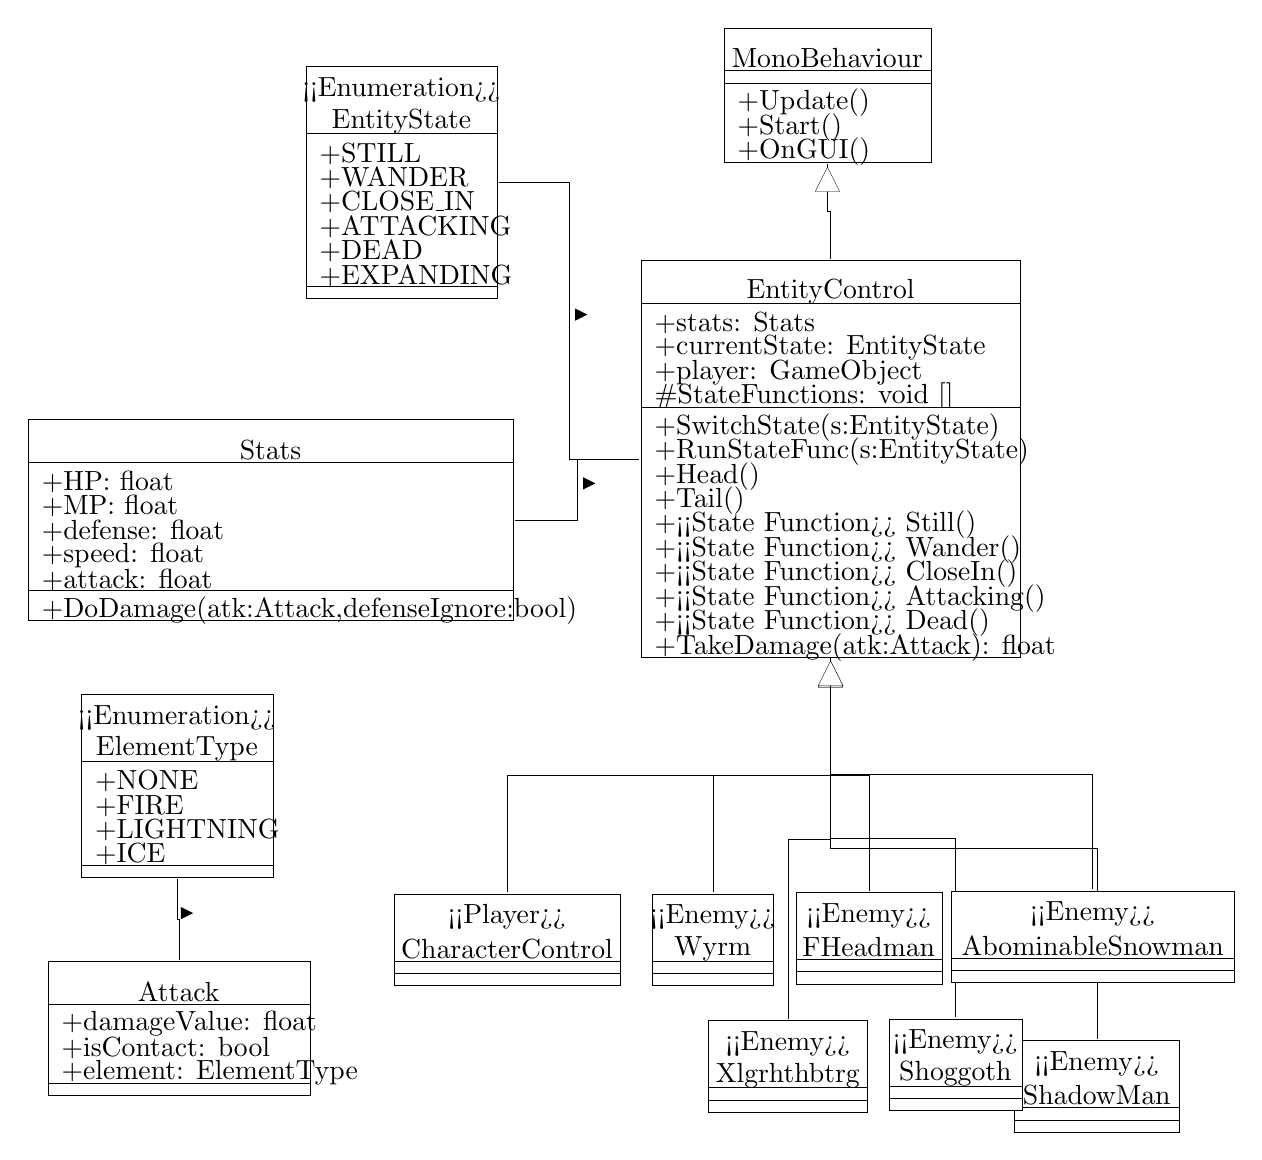
\begin{tikzpicture}
\pgftransformxscale{0.387817}
\pgftransformyscale{-0.387817}
\definecolor{dialinecolor}{rgb}{0.000000, 0.000000, 0.000000}
\pgfsetstrokecolor{dialinecolor}
\definecolor{dialinecolor}{rgb}{1.000000, 1.000000, 1.000000}
\pgfsetfillcolor{dialinecolor}
\pgfsetlinewidth{0.100000\du}
\pgfsetdash{}{0pt}
\definecolor{dialinecolor}{rgb}{1.000000, 1.000000, 1.000000}
\pgfsetfillcolor{dialinecolor}
\fill (-6.800000\du,4.250000\du)--(-6.800000\du,5.650000\du)--(5.635000\du,5.650000\du)--(5.635000\du,4.250000\du)--cycle;
\definecolor{dialinecolor}{rgb}{0.000000, 0.000000, 0.000000}
\pgfsetstrokecolor{dialinecolor}
\draw (-6.800000\du,4.250000\du)--(-6.800000\du,5.650000\du)--(5.635000\du,5.650000\du)--(5.635000\du,4.250000\du)--cycle;
% setfont left to latex
\definecolor{dialinecolor}{rgb}{0.000000, 0.000000, 0.000000}
\pgfsetstrokecolor{dialinecolor}
\node at (-0.582500\du,5.250000\du){EntityControl};
\definecolor{dialinecolor}{rgb}{1.000000, 1.000000, 1.000000}
\pgfsetfillcolor{dialinecolor}
\fill (-6.800000\du,5.650000\du)--(-6.800000\du,9.050000\du)--(5.635000\du,9.050000\du)--(5.635000\du,5.650000\du)--cycle;
\definecolor{dialinecolor}{rgb}{0.000000, 0.000000, 0.000000}
\pgfsetstrokecolor{dialinecolor}
\draw (-6.800000\du,5.650000\du)--(-6.800000\du,9.050000\du)--(5.635000\du,9.050000\du)--(5.635000\du,5.650000\du)--cycle;
% setfont left to latex
\definecolor{dialinecolor}{rgb}{0.000000, 0.000000, 0.000000}
\pgfsetstrokecolor{dialinecolor}
\node[anchor=west] at (-6.650000\du,6.310000\du){+stats: Stats};
% setfont left to latex
\definecolor{dialinecolor}{rgb}{0.000000, 0.000000, 0.000000}
\pgfsetstrokecolor{dialinecolor}
\node[anchor=west] at (-6.650000\du,7.110000\du){+currentState: EntityState};
% setfont left to latex
\definecolor{dialinecolor}{rgb}{0.000000, 0.000000, 0.000000}
\pgfsetstrokecolor{dialinecolor}
\node[anchor=west] at (-6.650000\du,7.910000\du){+player: GameObject};
% setfont left to latex
\definecolor{dialinecolor}{rgb}{0.000000, 0.000000, 0.000000}
\pgfsetstrokecolor{dialinecolor}
\node[anchor=west] at (-6.650000\du,8.710000\du){\#StateFunctions: void \ensuremath{[}\ensuremath{]}};
\definecolor{dialinecolor}{rgb}{1.000000, 1.000000, 1.000000}
\pgfsetfillcolor{dialinecolor}
\fill (-6.800000\du,9.050000\du)--(-6.800000\du,17.250000\du)--(5.635000\du,17.250000\du)--(5.635000\du,9.050000\du)--cycle;
\definecolor{dialinecolor}{rgb}{0.000000, 0.000000, 0.000000}
\pgfsetstrokecolor{dialinecolor}
\draw (-6.800000\du,9.050000\du)--(-6.800000\du,17.250000\du)--(5.635000\du,17.250000\du)--(5.635000\du,9.050000\du)--cycle;
% setfont left to latex
\definecolor{dialinecolor}{rgb}{0.000000, 0.000000, 0.000000}
\pgfsetstrokecolor{dialinecolor}
\node[anchor=west] at (-6.650000\du,9.710000\du){+SwitchState(s:EntityState)};
% setfont left to latex
\definecolor{dialinecolor}{rgb}{0.000000, 0.000000, 0.000000}
\pgfsetstrokecolor{dialinecolor}
\node[anchor=west] at (-6.650000\du,10.510000\du){+RunStateFunc(s:EntityState)};
% setfont left to latex
\definecolor{dialinecolor}{rgb}{0.000000, 0.000000, 0.000000}
\pgfsetstrokecolor{dialinecolor}
\node[anchor=west] at (-6.650000\du,11.310000\du){+Head()};
% setfont left to latex
\definecolor{dialinecolor}{rgb}{0.000000, 0.000000, 0.000000}
\pgfsetstrokecolor{dialinecolor}
\node[anchor=west] at (-6.650000\du,12.110000\du){+Tail()};
% setfont left to latex
\definecolor{dialinecolor}{rgb}{0.000000, 0.000000, 0.000000}
\pgfsetstrokecolor{dialinecolor}
\node[anchor=west] at (-6.650000\du,12.910000\du){+<<State Function>> Still()};
% setfont left to latex
\definecolor{dialinecolor}{rgb}{0.000000, 0.000000, 0.000000}
\pgfsetstrokecolor{dialinecolor}
\node[anchor=west] at (-6.650000\du,13.710000\du){+<<State Function>> Wander()};
% setfont left to latex
\definecolor{dialinecolor}{rgb}{0.000000, 0.000000, 0.000000}
\pgfsetstrokecolor{dialinecolor}
\node[anchor=west] at (-6.650000\du,14.510000\du){+<<State Function>> CloseIn()};
% setfont left to latex
\definecolor{dialinecolor}{rgb}{0.000000, 0.000000, 0.000000}
\pgfsetstrokecolor{dialinecolor}
\node[anchor=west] at (-6.650000\du,15.310000\du){+<<State Function>> Attacking()};
% setfont left to latex
\definecolor{dialinecolor}{rgb}{0.000000, 0.000000, 0.000000}
\pgfsetstrokecolor{dialinecolor}
\node[anchor=west] at (-6.650000\du,16.110000\du){+<<State Function>> Dead()};
% setfont left to latex
\definecolor{dialinecolor}{rgb}{0.000000, 0.000000, 0.000000}
\pgfsetstrokecolor{dialinecolor}
\node[anchor=west] at (-6.650000\du,16.910000\du){+TakeDamage(atk:Attack): float};
\pgfsetlinewidth{0.100000\du}
\pgfsetdash{}{0pt}
\definecolor{dialinecolor}{rgb}{1.000000, 1.000000, 1.000000}
\pgfsetfillcolor{dialinecolor}
\fill (-4.084275\du,-3.371875\du)--(-4.084275\du,-1.971875\du)--(2.710725\du,-1.971875\du)--(2.710725\du,-3.371875\du)--cycle;
\definecolor{dialinecolor}{rgb}{0.000000, 0.000000, 0.000000}
\pgfsetstrokecolor{dialinecolor}
\draw (-4.084275\du,-3.371875\du)--(-4.084275\du,-1.971875\du)--(2.710725\du,-1.971875\du)--(2.710725\du,-3.371875\du)--cycle;
% setfont left to latex
\definecolor{dialinecolor}{rgb}{0.000000, 0.000000, 0.000000}
\pgfsetstrokecolor{dialinecolor}
\node at (-0.686775\du,-2.371875\du){MonoBehaviour};
\definecolor{dialinecolor}{rgb}{1.000000, 1.000000, 1.000000}
\pgfsetfillcolor{dialinecolor}
\fill (-4.084275\du,-1.971875\du)--(-4.084275\du,-1.571875\du)--(2.710725\du,-1.571875\du)--(2.710725\du,-1.971875\du)--cycle;
\definecolor{dialinecolor}{rgb}{0.000000, 0.000000, 0.000000}
\pgfsetstrokecolor{dialinecolor}
\draw (-4.084275\du,-1.971875\du)--(-4.084275\du,-1.571875\du)--(2.710725\du,-1.571875\du)--(2.710725\du,-1.971875\du)--cycle;
\definecolor{dialinecolor}{rgb}{1.000000, 1.000000, 1.000000}
\pgfsetfillcolor{dialinecolor}
\fill (-4.084275\du,-1.571875\du)--(-4.084275\du,1.028125\du)--(2.710725\du,1.028125\du)--(2.710725\du,-1.571875\du)--cycle;
\definecolor{dialinecolor}{rgb}{0.000000, 0.000000, 0.000000}
\pgfsetstrokecolor{dialinecolor}
\draw (-4.084275\du,-1.571875\du)--(-4.084275\du,1.028125\du)--(2.710725\du,1.028125\du)--(2.710725\du,-1.571875\du)--cycle;
% setfont left to latex
\definecolor{dialinecolor}{rgb}{0.000000, 0.000000, 0.000000}
\pgfsetstrokecolor{dialinecolor}
\node[anchor=west] at (-3.934275\du,-0.911875\du){+Update()};
% setfont left to latex
\definecolor{dialinecolor}{rgb}{0.000000, 0.000000, 0.000000}
\pgfsetstrokecolor{dialinecolor}
\node[anchor=west] at (-3.934275\du,-0.111875\du){+Start()};
% setfont left to latex
\definecolor{dialinecolor}{rgb}{0.000000, 0.000000, 0.000000}
\pgfsetstrokecolor{dialinecolor}
\node[anchor=west] at (-3.934275\du,0.688125\du){+OnGUI()};
\pgfsetlinewidth{0.100000\du}
\pgfsetdash{}{0pt}
\pgfsetmiterjoin
\pgfsetbuttcap
{
\definecolor{dialinecolor}{rgb}{0.000000, 0.000000, 0.000000}
\pgfsetfillcolor{dialinecolor}
% was here!!!
\definecolor{dialinecolor}{rgb}{0.000000, 0.000000, 0.000000}
\pgfsetstrokecolor{dialinecolor}
\draw (-0.686775\du,1.078400\du)--(-0.686775\du,2.639000\du)--(-0.582500\du,2.639000\du)--(-0.582500\du,4.199600\du);
}
\definecolor{dialinecolor}{rgb}{0.000000, 0.000000, 0.000000}
\pgfsetstrokecolor{dialinecolor}
\draw (-0.686775\du,1.990203\du)--(-0.686775\du,2.639000\du)--(-0.582500\du,2.639000\du)--(-0.582500\du,4.199600\du);
\pgfsetmiterjoin
\definecolor{dialinecolor}{rgb}{1.000000, 1.000000, 1.000000}
\pgfsetfillcolor{dialinecolor}
\fill (-0.286775\du,1.990203\du)--(-0.686775\du,1.190203\du)--(-1.086775\du,1.990203\du)--cycle;
\pgfsetlinewidth{0.100000\du}
\pgfsetdash{}{0pt}
\pgfsetmiterjoin
\definecolor{dialinecolor}{rgb}{0.000000, 0.000000, 0.000000}
\pgfsetstrokecolor{dialinecolor}
\draw (-0.286775\du,1.990203\du)--(-0.686775\du,1.190203\du)--(-1.086775\du,1.990203\du)--cycle;
% setfont left to latex
\pgfsetlinewidth{0.100000\du}
\pgfsetdash{}{0pt}
\definecolor{dialinecolor}{rgb}{1.000000, 1.000000, 1.000000}
\pgfsetfillcolor{dialinecolor}
\fill (-17.771775\du,-2.109375\du)--(-17.771775\du,0.090625\du)--(-11.496775\du,0.090625\du)--(-11.496775\du,-2.109375\du)--cycle;
\definecolor{dialinecolor}{rgb}{0.000000, 0.000000, 0.000000}
\pgfsetstrokecolor{dialinecolor}
\draw (-17.771775\du,-2.109375\du)--(-17.771775\du,0.090625\du)--(-11.496775\du,0.090625\du)--(-11.496775\du,-2.109375\du)--cycle;
% setfont left to latex
\definecolor{dialinecolor}{rgb}{0.000000, 0.000000, 0.000000}
\pgfsetstrokecolor{dialinecolor}
\node at (-14.634275\du,-1.349375\du){<<Enumeration>>};
% setfont left to latex
\definecolor{dialinecolor}{rgb}{0.000000, 0.000000, 0.000000}
\pgfsetstrokecolor{dialinecolor}
\node at (-14.634275\du,-0.309375\du){EntityState};
\definecolor{dialinecolor}{rgb}{1.000000, 1.000000, 1.000000}
\pgfsetfillcolor{dialinecolor}
\fill (-17.771775\du,0.090625\du)--(-17.771775\du,5.090625\du)--(-11.496775\du,5.090625\du)--(-11.496775\du,0.090625\du)--cycle;
\definecolor{dialinecolor}{rgb}{0.000000, 0.000000, 0.000000}
\pgfsetstrokecolor{dialinecolor}
\draw (-17.771775\du,0.090625\du)--(-17.771775\du,5.090625\du)--(-11.496775\du,5.090625\du)--(-11.496775\du,0.090625\du)--cycle;
% setfont left to latex
\definecolor{dialinecolor}{rgb}{0.000000, 0.000000, 0.000000}
\pgfsetstrokecolor{dialinecolor}
\node[anchor=west] at (-17.621775\du,0.750625\du){+STILL};
% setfont left to latex
\definecolor{dialinecolor}{rgb}{0.000000, 0.000000, 0.000000}
\pgfsetstrokecolor{dialinecolor}
\node[anchor=west] at (-17.621775\du,1.550625\du){+WANDER};
% setfont left to latex
\definecolor{dialinecolor}{rgb}{0.000000, 0.000000, 0.000000}
\pgfsetstrokecolor{dialinecolor}
\node[anchor=west] at (-17.621775\du,2.350625\du){+CLOSE\_IN};
% setfont left to latex
\definecolor{dialinecolor}{rgb}{0.000000, 0.000000, 0.000000}
\pgfsetstrokecolor{dialinecolor}
\node[anchor=west] at (-17.621775\du,3.150625\du){+ATTACKING};
% setfont left to latex
\definecolor{dialinecolor}{rgb}{0.000000, 0.000000, 0.000000}
\pgfsetstrokecolor{dialinecolor}
\node[anchor=west] at (-17.621775\du,3.950625\du){+DEAD};
% setfont left to latex
\definecolor{dialinecolor}{rgb}{0.000000, 0.000000, 0.000000}
\pgfsetstrokecolor{dialinecolor}
\node[anchor=west] at (-17.621775\du,4.750625\du){+EXPANDING};
\definecolor{dialinecolor}{rgb}{1.000000, 1.000000, 1.000000}
\pgfsetfillcolor{dialinecolor}
\fill (-17.771775\du,5.090625\du)--(-17.771775\du,5.490625\du)--(-11.496775\du,5.490625\du)--(-11.496775\du,5.090625\du)--cycle;
\definecolor{dialinecolor}{rgb}{0.000000, 0.000000, 0.000000}
\pgfsetstrokecolor{dialinecolor}
\draw (-17.771775\du,5.090625\du)--(-17.771775\du,5.490625\du)--(-11.496775\du,5.490625\du)--(-11.496775\du,5.090625\du)--cycle;
\pgfsetlinewidth{0.100000\du}
\pgfsetdash{}{0pt}
\pgfsetmiterjoin
\pgfsetbuttcap
{
\definecolor{dialinecolor}{rgb}{0.000000, 0.000000, 0.000000}
\pgfsetfillcolor{dialinecolor}
% was here!!!
\definecolor{dialinecolor}{rgb}{0.000000, 0.000000, 0.000000}
\pgfsetstrokecolor{dialinecolor}
\draw (-11.446386\du,1.690625\du)--(-9.148384\du,1.690625\du)--(-9.148384\du,10.750000\du)--(-6.850383\du,10.750000\du);
}
% setfont left to latex
\definecolor{dialinecolor}{rgb}{0.000000, 0.000000, 0.000000}
\pgfsetfillcolor{dialinecolor}
\fill (-8.948384\du,6.220312\du)--(-8.948384\du,5.820312\du)--(-8.548384\du,6.020312\du)--cycle;
\pgfsetlinewidth{0.100000\du}
\pgfsetdash{}{0pt}
\definecolor{dialinecolor}{rgb}{1.000000, 1.000000, 1.000000}
\pgfsetfillcolor{dialinecolor}
\fill (-26.871775\du,9.440625\du)--(-26.871775\du,10.840625\du)--(-10.971775\du,10.840625\du)--(-10.971775\du,9.440625\du)--cycle;
\definecolor{dialinecolor}{rgb}{0.000000, 0.000000, 0.000000}
\pgfsetstrokecolor{dialinecolor}
\draw (-26.871775\du,9.440625\du)--(-26.871775\du,10.840625\du)--(-10.971775\du,10.840625\du)--(-10.971775\du,9.440625\du)--cycle;
% setfont left to latex
\definecolor{dialinecolor}{rgb}{0.000000, 0.000000, 0.000000}
\pgfsetstrokecolor{dialinecolor}
\node at (-18.921775\du,10.440625\du){Stats};
\definecolor{dialinecolor}{rgb}{1.000000, 1.000000, 1.000000}
\pgfsetfillcolor{dialinecolor}
\fill (-26.871775\du,10.840625\du)--(-26.871775\du,15.040625\du)--(-10.971775\du,15.040625\du)--(-10.971775\du,10.840625\du)--cycle;
\definecolor{dialinecolor}{rgb}{0.000000, 0.000000, 0.000000}
\pgfsetstrokecolor{dialinecolor}
\draw (-26.871775\du,10.840625\du)--(-26.871775\du,15.040625\du)--(-10.971775\du,15.040625\du)--(-10.971775\du,10.840625\du)--cycle;
% setfont left to latex
\definecolor{dialinecolor}{rgb}{0.000000, 0.000000, 0.000000}
\pgfsetstrokecolor{dialinecolor}
\node[anchor=west] at (-26.721775\du,11.500625\du){+HP: float};
% setfont left to latex
\definecolor{dialinecolor}{rgb}{0.000000, 0.000000, 0.000000}
\pgfsetstrokecolor{dialinecolor}
\node[anchor=west] at (-26.721775\du,12.300625\du){+MP: float};
% setfont left to latex
\definecolor{dialinecolor}{rgb}{0.000000, 0.000000, 0.000000}
\pgfsetstrokecolor{dialinecolor}
\node[anchor=west] at (-26.721775\du,13.100625\du){+defense: float};
% setfont left to latex
\definecolor{dialinecolor}{rgb}{0.000000, 0.000000, 0.000000}
\pgfsetstrokecolor{dialinecolor}
\node[anchor=west] at (-26.721775\du,13.900625\du){+speed: float};
% setfont left to latex
\definecolor{dialinecolor}{rgb}{0.000000, 0.000000, 0.000000}
\pgfsetstrokecolor{dialinecolor}
\node[anchor=west] at (-26.721775\du,14.700625\du){+attack: float};
\definecolor{dialinecolor}{rgb}{1.000000, 1.000000, 1.000000}
\pgfsetfillcolor{dialinecolor}
\fill (-26.871775\du,15.040625\du)--(-26.871775\du,16.040625\du)--(-10.971775\du,16.040625\du)--(-10.971775\du,15.040625\du)--cycle;
\definecolor{dialinecolor}{rgb}{0.000000, 0.000000, 0.000000}
\pgfsetstrokecolor{dialinecolor}
\draw (-26.871775\du,15.040625\du)--(-26.871775\du,16.040625\du)--(-10.971775\du,16.040625\du)--(-10.971775\du,15.040625\du)--cycle;
% setfont left to latex
\definecolor{dialinecolor}{rgb}{0.000000, 0.000000, 0.000000}
\pgfsetstrokecolor{dialinecolor}
\node[anchor=west] at (-26.721775\du,15.700625\du){+DoDamage(atk:Attack,defenseIgnore:bool)};
\pgfsetlinewidth{0.100000\du}
\pgfsetdash{}{0pt}
\definecolor{dialinecolor}{rgb}{1.000000, 1.000000, 1.000000}
\pgfsetfillcolor{dialinecolor}
\fill (-26.221775\du,27.190625\du)--(-26.221775\du,28.590625\du)--(-17.636775\du,28.590625\du)--(-17.636775\du,27.190625\du)--cycle;
\definecolor{dialinecolor}{rgb}{0.000000, 0.000000, 0.000000}
\pgfsetstrokecolor{dialinecolor}
\draw (-26.221775\du,27.190625\du)--(-26.221775\du,28.590625\du)--(-17.636775\du,28.590625\du)--(-17.636775\du,27.190625\du)--cycle;
% setfont left to latex
\definecolor{dialinecolor}{rgb}{0.000000, 0.000000, 0.000000}
\pgfsetstrokecolor{dialinecolor}
\node at (-21.929275\du,28.190625\du){Attack};
\definecolor{dialinecolor}{rgb}{1.000000, 1.000000, 1.000000}
\pgfsetfillcolor{dialinecolor}
\fill (-26.221775\du,28.590625\du)--(-26.221775\du,31.190625\du)--(-17.636775\du,31.190625\du)--(-17.636775\du,28.590625\du)--cycle;
\definecolor{dialinecolor}{rgb}{0.000000, 0.000000, 0.000000}
\pgfsetstrokecolor{dialinecolor}
\draw (-26.221775\du,28.590625\du)--(-26.221775\du,31.190625\du)--(-17.636775\du,31.190625\du)--(-17.636775\du,28.590625\du)--cycle;
% setfont left to latex
\definecolor{dialinecolor}{rgb}{0.000000, 0.000000, 0.000000}
\pgfsetstrokecolor{dialinecolor}
\node[anchor=west] at (-26.071775\du,29.250625\du){+damageValue: float};
% setfont left to latex
\definecolor{dialinecolor}{rgb}{0.000000, 0.000000, 0.000000}
\pgfsetstrokecolor{dialinecolor}
\node[anchor=west] at (-26.071775\du,30.050625\du){+isContact: bool};
% setfont left to latex
\definecolor{dialinecolor}{rgb}{0.000000, 0.000000, 0.000000}
\pgfsetstrokecolor{dialinecolor}
\node[anchor=west] at (-26.071775\du,30.850625\du){+element: ElementType};
\definecolor{dialinecolor}{rgb}{1.000000, 1.000000, 1.000000}
\pgfsetfillcolor{dialinecolor}
\fill (-26.221775\du,31.190625\du)--(-26.221775\du,31.590625\du)--(-17.636775\du,31.590625\du)--(-17.636775\du,31.190625\du)--cycle;
\definecolor{dialinecolor}{rgb}{0.000000, 0.000000, 0.000000}
\pgfsetstrokecolor{dialinecolor}
\draw (-26.221775\du,31.190625\du)--(-26.221775\du,31.590625\du)--(-17.636775\du,31.590625\du)--(-17.636775\du,31.190625\du)--cycle;
\pgfsetlinewidth{0.100000\du}
\pgfsetdash{}{0pt}
\definecolor{dialinecolor}{rgb}{1.000000, 1.000000, 1.000000}
\pgfsetfillcolor{dialinecolor}
\fill (-25.126775\du,18.445625\du)--(-25.126775\du,20.645625\du)--(-18.851775\du,20.645625\du)--(-18.851775\du,18.445625\du)--cycle;
\definecolor{dialinecolor}{rgb}{0.000000, 0.000000, 0.000000}
\pgfsetstrokecolor{dialinecolor}
\draw (-25.126775\du,18.445625\du)--(-25.126775\du,20.645625\du)--(-18.851775\du,20.645625\du)--(-18.851775\du,18.445625\du)--cycle;
% setfont left to latex
\definecolor{dialinecolor}{rgb}{0.000000, 0.000000, 0.000000}
\pgfsetstrokecolor{dialinecolor}
\node at (-21.989275\du,19.205625\du){<<Enumeration>>};
% setfont left to latex
\definecolor{dialinecolor}{rgb}{0.000000, 0.000000, 0.000000}
\pgfsetstrokecolor{dialinecolor}
\node at (-21.989275\du,20.245625\du){ElementType};
\definecolor{dialinecolor}{rgb}{1.000000, 1.000000, 1.000000}
\pgfsetfillcolor{dialinecolor}
\fill (-25.126775\du,20.645625\du)--(-25.126775\du,24.045625\du)--(-18.851775\du,24.045625\du)--(-18.851775\du,20.645625\du)--cycle;
\definecolor{dialinecolor}{rgb}{0.000000, 0.000000, 0.000000}
\pgfsetstrokecolor{dialinecolor}
\draw (-25.126775\du,20.645625\du)--(-25.126775\du,24.045625\du)--(-18.851775\du,24.045625\du)--(-18.851775\du,20.645625\du)--cycle;
% setfont left to latex
\definecolor{dialinecolor}{rgb}{0.000000, 0.000000, 0.000000}
\pgfsetstrokecolor{dialinecolor}
\node[anchor=west] at (-24.976775\du,21.305625\du){+NONE};
% setfont left to latex
\definecolor{dialinecolor}{rgb}{0.000000, 0.000000, 0.000000}
\pgfsetstrokecolor{dialinecolor}
\node[anchor=west] at (-24.976775\du,22.105625\du){+FIRE};
% setfont left to latex
\definecolor{dialinecolor}{rgb}{0.000000, 0.000000, 0.000000}
\pgfsetstrokecolor{dialinecolor}
\node[anchor=west] at (-24.976775\du,22.905625\du){+LIGHTNING};
% setfont left to latex
\definecolor{dialinecolor}{rgb}{0.000000, 0.000000, 0.000000}
\pgfsetstrokecolor{dialinecolor}
\node[anchor=west] at (-24.976775\du,23.705625\du){+ICE};
\definecolor{dialinecolor}{rgb}{1.000000, 1.000000, 1.000000}
\pgfsetfillcolor{dialinecolor}
\fill (-25.126775\du,24.045625\du)--(-25.126775\du,24.445625\du)--(-18.851775\du,24.445625\du)--(-18.851775\du,24.045625\du)--cycle;
\definecolor{dialinecolor}{rgb}{0.000000, 0.000000, 0.000000}
\pgfsetstrokecolor{dialinecolor}
\draw (-25.126775\du,24.045625\du)--(-25.126775\du,24.445625\du)--(-18.851775\du,24.445625\du)--(-18.851775\du,24.045625\du)--cycle;
\pgfsetlinewidth{0.100000\du}
\pgfsetdash{}{0pt}
\pgfsetmiterjoin
\pgfsetbuttcap
{
\definecolor{dialinecolor}{rgb}{0.000000, 0.000000, 0.000000}
\pgfsetfillcolor{dialinecolor}
% was here!!!
\definecolor{dialinecolor}{rgb}{0.000000, 0.000000, 0.000000}
\pgfsetstrokecolor{dialinecolor}
\draw (-21.929275\du,27.140350\du)--(-21.929275\du,25.818174\du)--(-21.989275\du,25.818174\du)--(-21.989275\du,24.495997\du);
}
% setfont left to latex
\definecolor{dialinecolor}{rgb}{0.000000, 0.000000, 0.000000}
\pgfsetfillcolor{dialinecolor}
\fill (-21.859275\du,25.818174\du)--(-21.859275\du,25.418174\du)--(-21.459275\du,25.618174\du)--cycle;
\pgfsetlinewidth{0.100000\du}
\pgfsetdash{}{0pt}
\pgfsetmiterjoin
\pgfsetbuttcap
{
\definecolor{dialinecolor}{rgb}{0.000000, 0.000000, 0.000000}
\pgfsetfillcolor{dialinecolor}
% was here!!!
\definecolor{dialinecolor}{rgb}{0.000000, 0.000000, 0.000000}
\pgfsetstrokecolor{dialinecolor}
\draw (-6.850383\du,10.750000\du)--(-8.885835\du,10.750000\du)--(-8.885835\du,12.740625\du)--(-10.921287\du,12.740625\du);
}
% setfont left to latex
\definecolor{dialinecolor}{rgb}{0.000000, 0.000000, 0.000000}
\pgfsetfillcolor{dialinecolor}
\fill (-8.685835\du,11.745312\du)--(-8.685835\du,11.345312\du)--(-8.285835\du,11.545312\du)--cycle;
\pgfsetlinewidth{0.100000\du}
\pgfsetdash{}{0pt}
\definecolor{dialinecolor}{rgb}{1.000000, 1.000000, 1.000000}
\pgfsetfillcolor{dialinecolor}
\fill (-1.726775\du,24.933125\du)--(-1.726775\du,27.133125\du)--(3.063225\du,27.133125\du)--(3.063225\du,24.933125\du)--cycle;
\definecolor{dialinecolor}{rgb}{0.000000, 0.000000, 0.000000}
\pgfsetstrokecolor{dialinecolor}
\draw (-1.726775\du,24.933125\du)--(-1.726775\du,27.133125\du)--(3.063225\du,27.133125\du)--(3.063225\du,24.933125\du)--cycle;
% setfont left to latex
\definecolor{dialinecolor}{rgb}{0.000000, 0.000000, 0.000000}
\pgfsetstrokecolor{dialinecolor}
\node at (0.668225\du,25.693125\du){<<Enemy>>};
% setfont left to latex
\definecolor{dialinecolor}{rgb}{0.000000, 0.000000, 0.000000}
\pgfsetstrokecolor{dialinecolor}
\node at (0.668225\du,26.733125\du){FHeadman};
\definecolor{dialinecolor}{rgb}{1.000000, 1.000000, 1.000000}
\pgfsetfillcolor{dialinecolor}
\fill (-1.726775\du,27.133125\du)--(-1.726775\du,27.533125\du)--(3.063225\du,27.533125\du)--(3.063225\du,27.133125\du)--cycle;
\definecolor{dialinecolor}{rgb}{0.000000, 0.000000, 0.000000}
\pgfsetstrokecolor{dialinecolor}
\draw (-1.726775\du,27.133125\du)--(-1.726775\du,27.533125\du)--(3.063225\du,27.533125\du)--(3.063225\du,27.133125\du)--cycle;
\definecolor{dialinecolor}{rgb}{1.000000, 1.000000, 1.000000}
\pgfsetfillcolor{dialinecolor}
\fill (-1.726775\du,27.533125\du)--(-1.726775\du,27.933125\du)--(3.063225\du,27.933125\du)--(3.063225\du,27.533125\du)--cycle;
\definecolor{dialinecolor}{rgb}{0.000000, 0.000000, 0.000000}
\pgfsetstrokecolor{dialinecolor}
\draw (-1.726775\du,27.533125\du)--(-1.726775\du,27.933125\du)--(3.063225\du,27.933125\du)--(3.063225\du,27.533125\du)--cycle;
\pgfsetlinewidth{0.100000\du}
\pgfsetdash{}{0pt}
\pgfsetmiterjoin
\pgfsetbuttcap
{
\definecolor{dialinecolor}{rgb}{0.000000, 0.000000, 0.000000}
\pgfsetfillcolor{dialinecolor}
% was here!!!
\definecolor{dialinecolor}{rgb}{0.000000, 0.000000, 0.000000}
\pgfsetstrokecolor{dialinecolor}
\draw (-0.582500\du,17.300400\du)--(-0.582500\du,21.091573\du)--(0.668225\du,21.091573\du)--(0.668225\du,24.882747\du);
}
\definecolor{dialinecolor}{rgb}{0.000000, 0.000000, 0.000000}
\pgfsetstrokecolor{dialinecolor}
\draw (-0.582500\du,18.212203\du)--(-0.582500\du,21.091573\du)--(0.668225\du,21.091573\du)--(0.668225\du,24.882747\du);
\pgfsetmiterjoin
\definecolor{dialinecolor}{rgb}{1.000000, 1.000000, 1.000000}
\pgfsetfillcolor{dialinecolor}
\fill (-0.182500\du,18.212203\du)--(-0.582500\du,17.412203\du)--(-0.982500\du,18.212203\du)--cycle;
\pgfsetlinewidth{0.100000\du}
\pgfsetdash{}{0pt}
\pgfsetmiterjoin
\definecolor{dialinecolor}{rgb}{0.000000, 0.000000, 0.000000}
\pgfsetstrokecolor{dialinecolor}
\draw (-0.182500\du,18.212203\du)--(-0.582500\du,17.412203\du)--(-0.982500\du,18.212203\du)--cycle;
% setfont left to latex
\pgfsetlinewidth{0.100000\du}
\pgfsetdash{}{0pt}
\definecolor{dialinecolor}{rgb}{1.000000, 1.000000, 1.000000}
\pgfsetfillcolor{dialinecolor}
\fill (5.423225\du,29.783125\du)--(5.423225\du,31.983125\du)--(10.840725\du,31.983125\du)--(10.840725\du,29.783125\du)--cycle;
\definecolor{dialinecolor}{rgb}{0.000000, 0.000000, 0.000000}
\pgfsetstrokecolor{dialinecolor}
\draw (5.423225\du,29.783125\du)--(5.423225\du,31.983125\du)--(10.840725\du,31.983125\du)--(10.840725\du,29.783125\du)--cycle;
% setfont left to latex
\definecolor{dialinecolor}{rgb}{0.000000, 0.000000, 0.000000}
\pgfsetstrokecolor{dialinecolor}
\node at (8.131975\du,30.543125\du){<<Enemy>>};
% setfont left to latex
\definecolor{dialinecolor}{rgb}{0.000000, 0.000000, 0.000000}
\pgfsetstrokecolor{dialinecolor}
\node at (8.131975\du,31.583125\du){ShadowMan};
\definecolor{dialinecolor}{rgb}{1.000000, 1.000000, 1.000000}
\pgfsetfillcolor{dialinecolor}
\fill (5.423225\du,31.983125\du)--(5.423225\du,32.383125\du)--(10.840725\du,32.383125\du)--(10.840725\du,31.983125\du)--cycle;
\definecolor{dialinecolor}{rgb}{0.000000, 0.000000, 0.000000}
\pgfsetstrokecolor{dialinecolor}
\draw (5.423225\du,31.983125\du)--(5.423225\du,32.383125\du)--(10.840725\du,32.383125\du)--(10.840725\du,31.983125\du)--cycle;
\definecolor{dialinecolor}{rgb}{1.000000, 1.000000, 1.000000}
\pgfsetfillcolor{dialinecolor}
\fill (5.423225\du,32.383125\du)--(5.423225\du,32.783125\du)--(10.840725\du,32.783125\du)--(10.840725\du,32.383125\du)--cycle;
\definecolor{dialinecolor}{rgb}{0.000000, 0.000000, 0.000000}
\pgfsetstrokecolor{dialinecolor}
\draw (5.423225\du,32.383125\du)--(5.423225\du,32.783125\du)--(10.840725\du,32.783125\du)--(10.840725\du,32.383125\du)--cycle;
\pgfsetlinewidth{0.100000\du}
\pgfsetdash{}{0pt}
\definecolor{dialinecolor}{rgb}{1.000000, 1.000000, 1.000000}
\pgfsetfillcolor{dialinecolor}
\fill (1.323225\du,29.083125\du)--(1.323225\du,31.283125\du)--(5.683225\du,31.283125\du)--(5.683225\du,29.083125\du)--cycle;
\definecolor{dialinecolor}{rgb}{0.000000, 0.000000, 0.000000}
\pgfsetstrokecolor{dialinecolor}
\draw (1.323225\du,29.083125\du)--(1.323225\du,31.283125\du)--(5.683225\du,31.283125\du)--(5.683225\du,29.083125\du)--cycle;
% setfont left to latex
\definecolor{dialinecolor}{rgb}{0.000000, 0.000000, 0.000000}
\pgfsetstrokecolor{dialinecolor}
\node at (3.503225\du,29.843125\du){<<Enemy>>};
% setfont left to latex
\definecolor{dialinecolor}{rgb}{0.000000, 0.000000, 0.000000}
\pgfsetstrokecolor{dialinecolor}
\node at (3.503225\du,30.883125\du){Shoggoth};
\definecolor{dialinecolor}{rgb}{1.000000, 1.000000, 1.000000}
\pgfsetfillcolor{dialinecolor}
\fill (1.323225\du,31.283125\du)--(1.323225\du,31.683125\du)--(5.683225\du,31.683125\du)--(5.683225\du,31.283125\du)--cycle;
\definecolor{dialinecolor}{rgb}{0.000000, 0.000000, 0.000000}
\pgfsetstrokecolor{dialinecolor}
\draw (1.323225\du,31.283125\du)--(1.323225\du,31.683125\du)--(5.683225\du,31.683125\du)--(5.683225\du,31.283125\du)--cycle;
\definecolor{dialinecolor}{rgb}{1.000000, 1.000000, 1.000000}
\pgfsetfillcolor{dialinecolor}
\fill (1.323225\du,31.683125\du)--(1.323225\du,32.083125\du)--(5.683225\du,32.083125\du)--(5.683225\du,31.683125\du)--cycle;
\definecolor{dialinecolor}{rgb}{0.000000, 0.000000, 0.000000}
\pgfsetstrokecolor{dialinecolor}
\draw (1.323225\du,31.683125\du)--(1.323225\du,32.083125\du)--(5.683225\du,32.083125\du)--(5.683225\du,31.683125\du)--cycle;
\pgfsetlinewidth{0.100000\du}
\pgfsetdash{}{0pt}
\definecolor{dialinecolor}{rgb}{1.000000, 1.000000, 1.000000}
\pgfsetfillcolor{dialinecolor}
\fill (-6.426775\du,24.983125\du)--(-6.426775\du,27.183125\du)--(-2.461775\du,27.183125\du)--(-2.461775\du,24.983125\du)--cycle;
\definecolor{dialinecolor}{rgb}{0.000000, 0.000000, 0.000000}
\pgfsetstrokecolor{dialinecolor}
\draw (-6.426775\du,24.983125\du)--(-6.426775\du,27.183125\du)--(-2.461775\du,27.183125\du)--(-2.461775\du,24.983125\du)--cycle;
% setfont left to latex
\definecolor{dialinecolor}{rgb}{0.000000, 0.000000, 0.000000}
\pgfsetstrokecolor{dialinecolor}
\node at (-4.444275\du,25.743125\du){<<Enemy>>};
% setfont left to latex
\definecolor{dialinecolor}{rgb}{0.000000, 0.000000, 0.000000}
\pgfsetstrokecolor{dialinecolor}
\node at (-4.444275\du,26.783125\du){Wyrm};
\definecolor{dialinecolor}{rgb}{1.000000, 1.000000, 1.000000}
\pgfsetfillcolor{dialinecolor}
\fill (-6.426775\du,27.183125\du)--(-6.426775\du,27.583125\du)--(-2.461775\du,27.583125\du)--(-2.461775\du,27.183125\du)--cycle;
\definecolor{dialinecolor}{rgb}{0.000000, 0.000000, 0.000000}
\pgfsetstrokecolor{dialinecolor}
\draw (-6.426775\du,27.183125\du)--(-6.426775\du,27.583125\du)--(-2.461775\du,27.583125\du)--(-2.461775\du,27.183125\du)--cycle;
\definecolor{dialinecolor}{rgb}{1.000000, 1.000000, 1.000000}
\pgfsetfillcolor{dialinecolor}
\fill (-6.426775\du,27.583125\du)--(-6.426775\du,27.983125\du)--(-2.461775\du,27.983125\du)--(-2.461775\du,27.583125\du)--cycle;
\definecolor{dialinecolor}{rgb}{0.000000, 0.000000, 0.000000}
\pgfsetstrokecolor{dialinecolor}
\draw (-6.426775\du,27.583125\du)--(-6.426775\du,27.983125\du)--(-2.461775\du,27.983125\du)--(-2.461775\du,27.583125\du)--cycle;
\pgfsetlinewidth{0.100000\du}
\pgfsetdash{}{0pt}
\pgfsetmiterjoin
\pgfsetbuttcap
{
\definecolor{dialinecolor}{rgb}{0.000000, 0.000000, 0.000000}
\pgfsetfillcolor{dialinecolor}
% was here!!!
\definecolor{dialinecolor}{rgb}{0.000000, 0.000000, 0.000000}
\pgfsetstrokecolor{dialinecolor}
\draw (-0.582500\du,17.300400\du)--(-0.582500\du,21.116573\du)--(-4.444275\du,21.116573\du)--(-4.444275\du,24.932747\du);
}
\definecolor{dialinecolor}{rgb}{0.000000, 0.000000, 0.000000}
\pgfsetstrokecolor{dialinecolor}
\draw (-0.582500\du,18.212203\du)--(-0.582500\du,21.116573\du)--(-4.444275\du,21.116573\du)--(-4.444275\du,24.932747\du);
\pgfsetmiterjoin
\definecolor{dialinecolor}{rgb}{1.000000, 1.000000, 1.000000}
\pgfsetfillcolor{dialinecolor}
\fill (-0.182500\du,18.212203\du)--(-0.582500\du,17.412203\du)--(-0.982500\du,18.212203\du)--cycle;
\pgfsetlinewidth{0.100000\du}
\pgfsetdash{}{0pt}
\pgfsetmiterjoin
\definecolor{dialinecolor}{rgb}{0.000000, 0.000000, 0.000000}
\pgfsetstrokecolor{dialinecolor}
\draw (-0.182500\du,18.212203\du)--(-0.582500\du,17.412203\du)--(-0.982500\du,18.212203\du)--cycle;
% setfont left to latex
\pgfsetlinewidth{0.100000\du}
\pgfsetdash{}{0pt}
\pgfsetmiterjoin
\pgfsetbuttcap
{
\definecolor{dialinecolor}{rgb}{0.000000, 0.000000, 0.000000}
\pgfsetfillcolor{dialinecolor}
% was here!!!
\definecolor{dialinecolor}{rgb}{0.000000, 0.000000, 0.000000}
\pgfsetstrokecolor{dialinecolor}
\draw (-0.582500\du,17.250000\du)--(-0.582500\du,23.491373\du)--(8.131975\du,23.491373\du)--(8.131975\du,29.732747\du);
}
\definecolor{dialinecolor}{rgb}{0.000000, 0.000000, 0.000000}
\pgfsetstrokecolor{dialinecolor}
\draw (-0.582500\du,18.161803\du)--(-0.582500\du,23.491373\du)--(8.131975\du,23.491373\du)--(8.131975\du,29.732747\du);
\pgfsetmiterjoin
\definecolor{dialinecolor}{rgb}{1.000000, 1.000000, 1.000000}
\pgfsetfillcolor{dialinecolor}
\fill (-0.182500\du,18.161803\du)--(-0.582500\du,17.361803\du)--(-0.982500\du,18.161803\du)--cycle;
\pgfsetlinewidth{0.100000\du}
\pgfsetdash{}{0pt}
\pgfsetmiterjoin
\definecolor{dialinecolor}{rgb}{0.000000, 0.000000, 0.000000}
\pgfsetstrokecolor{dialinecolor}
\draw (-0.182500\du,18.161803\du)--(-0.582500\du,17.361803\du)--(-0.982500\du,18.161803\du)--cycle;
% setfont left to latex
\pgfsetlinewidth{0.100000\du}
\pgfsetdash{}{0pt}
\pgfsetmiterjoin
\pgfsetbuttcap
{
\definecolor{dialinecolor}{rgb}{0.000000, 0.000000, 0.000000}
\pgfsetfillcolor{dialinecolor}
% was here!!!
\definecolor{dialinecolor}{rgb}{0.000000, 0.000000, 0.000000}
\pgfsetstrokecolor{dialinecolor}
\draw (-0.582500\du,17.300400\du)--(-0.582500\du,23.166573\du)--(3.503225\du,23.166573\du)--(3.503225\du,29.032747\du);
}
\definecolor{dialinecolor}{rgb}{0.000000, 0.000000, 0.000000}
\pgfsetstrokecolor{dialinecolor}
\draw (-0.582500\du,18.212203\du)--(-0.582500\du,23.166573\du)--(3.503225\du,23.166573\du)--(3.503225\du,29.032747\du);
\pgfsetmiterjoin
\definecolor{dialinecolor}{rgb}{1.000000, 1.000000, 1.000000}
\pgfsetfillcolor{dialinecolor}
\fill (-0.182500\du,18.212203\du)--(-0.582500\du,17.412203\du)--(-0.982500\du,18.212203\du)--cycle;
\pgfsetlinewidth{0.100000\du}
\pgfsetdash{}{0pt}
\pgfsetmiterjoin
\definecolor{dialinecolor}{rgb}{0.000000, 0.000000, 0.000000}
\pgfsetstrokecolor{dialinecolor}
\draw (-0.182500\du,18.212203\du)--(-0.582500\du,17.412203\du)--(-0.982500\du,18.212203\du)--cycle;
% setfont left to latex
\pgfsetlinewidth{0.100000\du}
\pgfsetdash{}{0pt}
\definecolor{dialinecolor}{rgb}{1.000000, 1.000000, 1.000000}
\pgfsetfillcolor{dialinecolor}
\fill (3.373225\du,24.883125\du)--(3.373225\du,27.083125\du)--(12.623225\du,27.083125\du)--(12.623225\du,24.883125\du)--cycle;
\definecolor{dialinecolor}{rgb}{0.000000, 0.000000, 0.000000}
\pgfsetstrokecolor{dialinecolor}
\draw (3.373225\du,24.883125\du)--(3.373225\du,27.083125\du)--(12.623225\du,27.083125\du)--(12.623225\du,24.883125\du)--cycle;
% setfont left to latex
\definecolor{dialinecolor}{rgb}{0.000000, 0.000000, 0.000000}
\pgfsetstrokecolor{dialinecolor}
\node at (7.998225\du,25.643125\du){<<Enemy>>};
% setfont left to latex
\definecolor{dialinecolor}{rgb}{0.000000, 0.000000, 0.000000}
\pgfsetstrokecolor{dialinecolor}
\node at (7.998225\du,26.683125\du){AbominableSnowman};
\definecolor{dialinecolor}{rgb}{1.000000, 1.000000, 1.000000}
\pgfsetfillcolor{dialinecolor}
\fill (3.373225\du,27.083125\du)--(3.373225\du,27.483125\du)--(12.623225\du,27.483125\du)--(12.623225\du,27.083125\du)--cycle;
\definecolor{dialinecolor}{rgb}{0.000000, 0.000000, 0.000000}
\pgfsetstrokecolor{dialinecolor}
\draw (3.373225\du,27.083125\du)--(3.373225\du,27.483125\du)--(12.623225\du,27.483125\du)--(12.623225\du,27.083125\du)--cycle;
\definecolor{dialinecolor}{rgb}{1.000000, 1.000000, 1.000000}
\pgfsetfillcolor{dialinecolor}
\fill (3.373225\du,27.483125\du)--(3.373225\du,27.883125\du)--(12.623225\du,27.883125\du)--(12.623225\du,27.483125\du)--cycle;
\definecolor{dialinecolor}{rgb}{0.000000, 0.000000, 0.000000}
\pgfsetstrokecolor{dialinecolor}
\draw (3.373225\du,27.483125\du)--(3.373225\du,27.883125\du)--(12.623225\du,27.883125\du)--(12.623225\du,27.483125\du)--cycle;
\pgfsetlinewidth{0.100000\du}
\pgfsetdash{}{0pt}
\pgfsetmiterjoin
\pgfsetbuttcap
{
\definecolor{dialinecolor}{rgb}{0.000000, 0.000000, 0.000000}
\pgfsetfillcolor{dialinecolor}
% was here!!!
\definecolor{dialinecolor}{rgb}{0.000000, 0.000000, 0.000000}
\pgfsetstrokecolor{dialinecolor}
\draw (-0.582500\du,17.300400\du)--(-0.582500\du,21.066573\du)--(7.998225\du,21.066573\du)--(7.998225\du,24.832747\du);
}
\definecolor{dialinecolor}{rgb}{0.000000, 0.000000, 0.000000}
\pgfsetstrokecolor{dialinecolor}
\draw (-0.582500\du,18.212203\du)--(-0.582500\du,21.066573\du)--(7.998225\du,21.066573\du)--(7.998225\du,24.832747\du);
\pgfsetmiterjoin
\definecolor{dialinecolor}{rgb}{1.000000, 1.000000, 1.000000}
\pgfsetfillcolor{dialinecolor}
\fill (-0.182500\du,18.212203\du)--(-0.582500\du,17.412203\du)--(-0.982500\du,18.212203\du)--cycle;
\pgfsetlinewidth{0.100000\du}
\pgfsetdash{}{0pt}
\pgfsetmiterjoin
\definecolor{dialinecolor}{rgb}{0.000000, 0.000000, 0.000000}
\pgfsetstrokecolor{dialinecolor}
\draw (-0.182500\du,18.212203\du)--(-0.582500\du,17.412203\du)--(-0.982500\du,18.212203\du)--cycle;
% setfont left to latex
\pgfsetlinewidth{0.100000\du}
\pgfsetdash{}{0pt}
\definecolor{dialinecolor}{rgb}{1.000000, 1.000000, 1.000000}
\pgfsetfillcolor{dialinecolor}
\fill (-4.576775\du,29.133125\du)--(-4.576775\du,31.333125\du)--(0.608225\du,31.333125\du)--(0.608225\du,29.133125\du)--cycle;
\definecolor{dialinecolor}{rgb}{0.000000, 0.000000, 0.000000}
\pgfsetstrokecolor{dialinecolor}
\draw (-4.576775\du,29.133125\du)--(-4.576775\du,31.333125\du)--(0.608225\du,31.333125\du)--(0.608225\du,29.133125\du)--cycle;
% setfont left to latex
\definecolor{dialinecolor}{rgb}{0.000000, 0.000000, 0.000000}
\pgfsetstrokecolor{dialinecolor}
\node at (-1.984275\du,29.893125\du){<<Enemy>>};
% setfont left to latex
\definecolor{dialinecolor}{rgb}{0.000000, 0.000000, 0.000000}
\pgfsetstrokecolor{dialinecolor}
\node at (-1.984275\du,30.933125\du){Xlgrhthbtrg};
\definecolor{dialinecolor}{rgb}{1.000000, 1.000000, 1.000000}
\pgfsetfillcolor{dialinecolor}
\fill (-4.576775\du,31.333125\du)--(-4.576775\du,31.733125\du)--(0.608225\du,31.733125\du)--(0.608225\du,31.333125\du)--cycle;
\definecolor{dialinecolor}{rgb}{0.000000, 0.000000, 0.000000}
\pgfsetstrokecolor{dialinecolor}
\draw (-4.576775\du,31.333125\du)--(-4.576775\du,31.733125\du)--(0.608225\du,31.733125\du)--(0.608225\du,31.333125\du)--cycle;
\definecolor{dialinecolor}{rgb}{1.000000, 1.000000, 1.000000}
\pgfsetfillcolor{dialinecolor}
\fill (-4.576775\du,31.733125\du)--(-4.576775\du,32.133125\du)--(0.608225\du,32.133125\du)--(0.608225\du,31.733125\du)--cycle;
\definecolor{dialinecolor}{rgb}{0.000000, 0.000000, 0.000000}
\pgfsetstrokecolor{dialinecolor}
\draw (-4.576775\du,31.733125\du)--(-4.576775\du,32.133125\du)--(0.608225\du,32.133125\du)--(0.608225\du,31.733125\du)--cycle;
\pgfsetlinewidth{0.100000\du}
\pgfsetdash{}{0pt}
\pgfsetmiterjoin
\pgfsetbuttcap
{
\definecolor{dialinecolor}{rgb}{0.000000, 0.000000, 0.000000}
\pgfsetfillcolor{dialinecolor}
% was here!!!
\definecolor{dialinecolor}{rgb}{0.000000, 0.000000, 0.000000}
\pgfsetstrokecolor{dialinecolor}
\draw (-0.582500\du,17.300400\du)--(-0.582500\du,23.191573\du)--(-1.984275\du,23.191573\du)--(-1.984275\du,29.082747\du);
}
\definecolor{dialinecolor}{rgb}{0.000000, 0.000000, 0.000000}
\pgfsetstrokecolor{dialinecolor}
\draw (-0.582500\du,18.212203\du)--(-0.582500\du,23.191573\du)--(-1.984275\du,23.191573\du)--(-1.984275\du,29.082747\du);
\pgfsetmiterjoin
\definecolor{dialinecolor}{rgb}{1.000000, 1.000000, 1.000000}
\pgfsetfillcolor{dialinecolor}
\fill (-0.182500\du,18.212203\du)--(-0.582500\du,17.412203\du)--(-0.982500\du,18.212203\du)--cycle;
\pgfsetlinewidth{0.100000\du}
\pgfsetdash{}{0pt}
\pgfsetmiterjoin
\definecolor{dialinecolor}{rgb}{0.000000, 0.000000, 0.000000}
\pgfsetstrokecolor{dialinecolor}
\draw (-0.182500\du,18.212203\du)--(-0.582500\du,17.412203\du)--(-0.982500\du,18.212203\du)--cycle;
% setfont left to latex
\pgfsetlinewidth{0.100000\du}
\pgfsetdash{}{0pt}
\definecolor{dialinecolor}{rgb}{1.000000, 1.000000, 1.000000}
\pgfsetfillcolor{dialinecolor}
\fill (-14.876775\du,24.983125\du)--(-14.876775\du,27.183125\du)--(-7.484275\du,27.183125\du)--(-7.484275\du,24.983125\du)--cycle;
\definecolor{dialinecolor}{rgb}{0.000000, 0.000000, 0.000000}
\pgfsetstrokecolor{dialinecolor}
\draw (-14.876775\du,24.983125\du)--(-14.876775\du,27.183125\du)--(-7.484275\du,27.183125\du)--(-7.484275\du,24.983125\du)--cycle;
% setfont left to latex
\definecolor{dialinecolor}{rgb}{0.000000, 0.000000, 0.000000}
\pgfsetstrokecolor{dialinecolor}
\node at (-11.180525\du,25.743125\du){<<Player>>};
% setfont left to latex
\definecolor{dialinecolor}{rgb}{0.000000, 0.000000, 0.000000}
\pgfsetstrokecolor{dialinecolor}
\node at (-11.180525\du,26.783125\du){CharacterControl};
\definecolor{dialinecolor}{rgb}{1.000000, 1.000000, 1.000000}
\pgfsetfillcolor{dialinecolor}
\fill (-14.876775\du,27.183125\du)--(-14.876775\du,27.583125\du)--(-7.484275\du,27.583125\du)--(-7.484275\du,27.183125\du)--cycle;
\definecolor{dialinecolor}{rgb}{0.000000, 0.000000, 0.000000}
\pgfsetstrokecolor{dialinecolor}
\draw (-14.876775\du,27.183125\du)--(-14.876775\du,27.583125\du)--(-7.484275\du,27.583125\du)--(-7.484275\du,27.183125\du)--cycle;
\definecolor{dialinecolor}{rgb}{1.000000, 1.000000, 1.000000}
\pgfsetfillcolor{dialinecolor}
\fill (-14.876775\du,27.583125\du)--(-14.876775\du,27.983125\du)--(-7.484275\du,27.983125\du)--(-7.484275\du,27.583125\du)--cycle;
\definecolor{dialinecolor}{rgb}{0.000000, 0.000000, 0.000000}
\pgfsetstrokecolor{dialinecolor}
\draw (-14.876775\du,27.583125\du)--(-14.876775\du,27.983125\du)--(-7.484275\du,27.983125\du)--(-7.484275\du,27.583125\du)--cycle;
\pgfsetlinewidth{0.100000\du}
\pgfsetdash{}{0pt}
\pgfsetmiterjoin
\pgfsetbuttcap
{
\definecolor{dialinecolor}{rgb}{0.000000, 0.000000, 0.000000}
\pgfsetfillcolor{dialinecolor}
% was here!!!
\definecolor{dialinecolor}{rgb}{0.000000, 0.000000, 0.000000}
\pgfsetstrokecolor{dialinecolor}
\draw (-0.582500\du,17.250000\du)--(-0.582500\du,21.091373\du)--(-11.180525\du,21.091373\du)--(-11.180525\du,24.932747\du);
}
\definecolor{dialinecolor}{rgb}{0.000000, 0.000000, 0.000000}
\pgfsetstrokecolor{dialinecolor}
\draw (-0.582500\du,18.161803\du)--(-0.582500\du,21.091373\du)--(-11.180525\du,21.091373\du)--(-11.180525\du,24.932747\du);
\pgfsetmiterjoin
\definecolor{dialinecolor}{rgb}{1.000000, 1.000000, 1.000000}
\pgfsetfillcolor{dialinecolor}
\fill (-0.182500\du,18.161803\du)--(-0.582500\du,17.361803\du)--(-0.982500\du,18.161803\du)--cycle;
\pgfsetlinewidth{0.100000\du}
\pgfsetdash{}{0pt}
\pgfsetmiterjoin
\definecolor{dialinecolor}{rgb}{0.000000, 0.000000, 0.000000}
\pgfsetstrokecolor{dialinecolor}
\draw (-0.182500\du,18.161803\du)--(-0.582500\du,17.361803\du)--(-0.982500\du,18.161803\du)--cycle;
% setfont left to latex
\end{tikzpicture}

}
\caption{A UML diagram of the entity control and combat system.}
\label{AI_Combat}
\end{figure}








\subsection{Game Flow}

The flow of control in code as it relates to the AI and Combat systems will be described in this section.  The classes and systems referred to in thie section were introduced in the previous section.

\subsubsection{State Machines and AI}

During the Start function (a function of MonoBehaviour that is run when a game object is initialized), the StateFunctions array of an EntityControl object is automatically initialized to default values.  During this stage, some indices of the array are matched up with their default functions (those marked as "State Function" in the UML diagram).  These functions represent states that tend to be universal across all entities.  Some indices of the array correspond to more specific states, and are therefore not initialized.  This is done so that exceptions will be thrown for invalid states, allowing bugs in code to be caught more effectively.

The Update method in EntityControl functions primarily as a state function dispatcher.  Rather than use the Update method directly in the subclasses, hooks are provided to allow more organization.  Flow of control is illustrated in Fig \ref{UpdateCycle}.  First, the Head function is called to execute any code that may be required before the state function.  Next, the current state function is fetched from the array.  If there is no function for the current state, and exception is thrown and execution stops.  Otherwise, the current state function is executed.  Control continues to the Tail method, executing any code that may be required at the end of the update cycle.

\begin{figure}[h!]
{\scalefont{0.8}
% Graphic for TeX using PGF
% Title: C:\Users\Kaylen\CotWM\Doc\UML\UpdateCycle.dia
% Creator: Dia v0.97.1
% CreationDate: Sat Mar 10 19:22:49 2012
% For: Kaylen
% \usepackage{tikz}
% The following commands are not supported in PSTricks at present
% We define them conditionally, so when they are implemented,
% this pgf file will use them.
\ifx\du\undefined
  \newlength{\du}
\fi
\setlength{\du}{15\unitlength}
\begin{tikzpicture}
\pgftransformxscale{0.865104}
\pgftransformyscale{-0.865104}
\definecolor{dialinecolor}{rgb}{0.000000, 0.000000, 0.000000}
\pgfsetstrokecolor{dialinecolor}
\definecolor{dialinecolor}{rgb}{1.000000, 1.000000, 1.000000}
\pgfsetfillcolor{dialinecolor}
\pgfsetlinewidth{0.100000\du}
\pgfsetdash{}{0pt}
\definecolor{dialinecolor}{rgb}{1.000000, 1.000000, 1.000000}
\pgfsetfillcolor{dialinecolor}
\fill (12.087500\du,-3.462500\du)--(12.087500\du,18.087500\du)--(29.737500\du,18.087500\du)--(29.737500\du,-3.462500\du)--cycle;
\definecolor{dialinecolor}{rgb}{0.000000, 0.000000, 0.000000}
\pgfsetstrokecolor{dialinecolor}
\draw (12.087500\du,-3.462500\du)--(12.087500\du,18.087500\du)--(29.737500\du,18.087500\du)--(29.737500\du,-3.462500\du)--cycle;
\definecolor{dialinecolor}{rgb}{1.000000, 1.000000, 1.000000}
\pgfsetfillcolor{dialinecolor}
\fill (12.087500\du,-4.462500\du)--(12.087500\du,-3.462500\du)--(14.597500\du,-3.462500\du)--(14.597500\du,-4.462500\du)--cycle;
\definecolor{dialinecolor}{rgb}{0.000000, 0.000000, 0.000000}
\pgfsetstrokecolor{dialinecolor}
\draw (12.087500\du,-4.462500\du)--(12.087500\du,-3.462500\du)--(14.597500\du,-3.462500\du)--(14.597500\du,-4.462500\du)--cycle;
% setfont left to latex
\definecolor{dialinecolor}{rgb}{0.000000, 0.000000, 0.000000}
\pgfsetstrokecolor{dialinecolor}
\node[anchor=west] at (12.187500\du,-3.762500\du){Update};
\pgfsetlinewidth{0.100000\du}
\pgfsetdash{}{0pt}
\definecolor{dialinecolor}{rgb}{0.000000, 0.000000, 0.000000}
\pgfsetfillcolor{dialinecolor}
\pgfpathellipse{\pgfpoint{19.000000\du}{-4.650000\du}}{\pgfpoint{0.500000\du}{0\du}}{\pgfpoint{0\du}{0.500000\du}}
\pgfusepath{fill}
\pgfsetlinewidth{0.100000\du}
\pgfsetdash{}{0pt}
{\pgfsetcornersarced{\pgfpoint{1.000000\du}{1.000000\du}}\definecolor{dialinecolor}{rgb}{1.000000, 1.000000, 1.000000}
\pgfsetfillcolor{dialinecolor}
\fill (16.987500\du,-0.612500\du)--(16.987500\du,1.187500\du)--(20.987500\du,1.187500\du)--(20.987500\du,-0.612500\du)--cycle;
}{\pgfsetcornersarced{\pgfpoint{1.000000\du}{1.000000\du}}\definecolor{dialinecolor}{rgb}{0.000000, 0.000000, 0.000000}
\pgfsetstrokecolor{dialinecolor}
\draw (16.987500\du,-0.612500\du)--(16.987500\du,1.187500\du)--(20.987500\du,1.187500\du)--(20.987500\du,-0.612500\du)--cycle;
}% setfont left to latex
\definecolor{dialinecolor}{rgb}{0.000000, 0.000000, 0.000000}
\pgfsetstrokecolor{dialinecolor}
\node at (18.987500\du,0.527500\du){Head()};
\pgfsetlinewidth{0.100000\du}
\pgfsetdash{}{0pt}
{\pgfsetcornersarced{\pgfpoint{1.000000\du}{1.000000\du}}\definecolor{dialinecolor}{rgb}{1.000000, 1.000000, 1.000000}
\pgfsetfillcolor{dialinecolor}
\fill (16.982500\du,14.742500\du)--(16.982500\du,16.542500\du)--(20.982500\du,16.542500\du)--(20.982500\du,14.742500\du)--cycle;
}{\pgfsetcornersarced{\pgfpoint{1.000000\du}{1.000000\du}}\definecolor{dialinecolor}{rgb}{0.000000, 0.000000, 0.000000}
\pgfsetstrokecolor{dialinecolor}
\draw (16.982500\du,14.742500\du)--(16.982500\du,16.542500\du)--(20.982500\du,16.542500\du)--(20.982500\du,14.742500\du)--cycle;
}% setfont left to latex
\definecolor{dialinecolor}{rgb}{0.000000, 0.000000, 0.000000}
\pgfsetstrokecolor{dialinecolor}
\node at (18.982500\du,15.882500\du){Tail()};
\pgfsetlinewidth{0.100000\du}
\pgfsetdash{}{0pt}
{\pgfsetcornersarced{\pgfpoint{1.000000\du}{1.000000\du}}\definecolor{dialinecolor}{rgb}{1.000000, 1.000000, 1.000000}
\pgfsetfillcolor{dialinecolor}
\fill (23.277500\du,3.747500\du)--(23.277500\du,5.547500\du)--(28.835000\du,5.547500\du)--(28.835000\du,3.747500\du)--cycle;
}{\pgfsetcornersarced{\pgfpoint{1.000000\du}{1.000000\du}}\definecolor{dialinecolor}{rgb}{0.000000, 0.000000, 0.000000}
\pgfsetstrokecolor{dialinecolor}
\draw (23.277500\du,3.747500\du)--(23.277500\du,5.547500\du)--(28.835000\du,5.547500\du)--(28.835000\du,3.747500\du)--cycle;
}% setfont left to latex
\definecolor{dialinecolor}{rgb}{0.000000, 0.000000, 0.000000}
\pgfsetstrokecolor{dialinecolor}
\node at (26.056250\du,4.887500\du){throw Exception};
\pgfsetlinewidth{0.100000\du}
\pgfsetdash{}{0pt}
\definecolor{dialinecolor}{rgb}{1.000000, 1.000000, 1.000000}
\pgfsetfillcolor{dialinecolor}
\fill (17.987500\du,4.637500\du)--(18.987500\du,3.637500\du)--(19.987500\du,4.637500\du)--(18.987500\du,5.637500\du)--cycle;
\definecolor{dialinecolor}{rgb}{0.000000, 0.000000, 0.000000}
\pgfsetstrokecolor{dialinecolor}
\draw (17.987500\du,4.637500\du)--(18.987500\du,3.637500\du)--(19.987500\du,4.637500\du)--(18.987500\du,5.637500\du)--cycle;
\pgfsetlinewidth{0.100000\du}
\pgfsetbuttcap
\pgfsetdash{}{0pt}
{
\definecolor{dialinecolor}{rgb}{0.000000, 0.000000, 0.000000}
\pgfsetfillcolor{dialinecolor}
% was here!!!
\pgfsetarrowsend{to}
\definecolor{dialinecolor}{rgb}{0.000000, 0.000000, 0.000000}
\pgfsetstrokecolor{dialinecolor}
\draw (19.000000\du,-4.099731\du)--(19.000000\du,-2.356116\du)--(18.987500\du,-2.356116\du)--(18.987500\du,-0.612500\du);
}
% setfont left to latex
\pgfsetlinewidth{0.100000\du}
\pgfsetbuttcap
\pgfsetdash{}{0pt}
{
\definecolor{dialinecolor}{rgb}{0.000000, 0.000000, 0.000000}
\pgfsetfillcolor{dialinecolor}
% was here!!!
\pgfsetarrowsend{to}
\definecolor{dialinecolor}{rgb}{0.000000, 0.000000, 0.000000}
\pgfsetstrokecolor{dialinecolor}
\draw (18.987500\du,1.187500\du)--(18.987500\du,1.187500\du)--(18.987500\du,3.637500\du)--(18.987500\du,3.637500\du);
}
% setfont left to latex
\pgfsetlinewidth{0.100000\du}
\pgfsetbuttcap
\pgfsetdash{}{0pt}
{
\definecolor{dialinecolor}{rgb}{0.000000, 0.000000, 0.000000}
\pgfsetfillcolor{dialinecolor}
% was here!!!
\pgfsetarrowsend{to}
\definecolor{dialinecolor}{rgb}{0.000000, 0.000000, 0.000000}
\pgfsetstrokecolor{dialinecolor}
\draw (18.987500\du,5.637500\du)--(18.987500\du,5.637500\du)--(18.987500\du,9.942500\du)--(18.987500\du,9.942500\du);
}
% setfont left to latex
\definecolor{dialinecolor}{rgb}{0.000000, 0.000000, 0.000000}
\pgfsetstrokecolor{dialinecolor}
\node at (18.487500\du,7.290000\du){\ensuremath{[}StateFunctions\ensuremath{[}CurrentState\ensuremath{]} != null\ensuremath{]}};
\pgfsetlinewidth{0.100000\du}
\pgfsetbuttcap
\pgfsetdash{}{0pt}
{
\definecolor{dialinecolor}{rgb}{0.000000, 0.000000, 0.000000}
\pgfsetfillcolor{dialinecolor}
% was here!!!
\pgfsetarrowsend{to}
\definecolor{dialinecolor}{rgb}{0.000000, 0.000000, 0.000000}
\pgfsetstrokecolor{dialinecolor}
\draw (19.987500\du,4.637500\du)--(21.632500\du,4.637500\du)--(21.632500\du,4.647500\du)--(23.277500\du,4.647500\du);
}
% setfont left to latex
\definecolor{dialinecolor}{rgb}{0.000000, 0.000000, 0.000000}
\pgfsetstrokecolor{dialinecolor}
\node at (21.132500\du,4.142500\du){\ensuremath{[}else\ensuremath{]}};
\pgfsetlinewidth{0.100000\du}
\pgfsetdash{}{0pt}
{\pgfsetcornersarced{\pgfpoint{1.000000\du}{1.000000\du}}\definecolor{dialinecolor}{rgb}{1.000000, 1.000000, 1.000000}
\pgfsetfillcolor{dialinecolor}
\fill (14.132500\du,9.942500\du)--(14.132500\du,11.742500\du)--(23.842500\du,11.742500\du)--(23.842500\du,9.942500\du)--cycle;
}{\pgfsetcornersarced{\pgfpoint{1.000000\du}{1.000000\du}}\definecolor{dialinecolor}{rgb}{0.000000, 0.000000, 0.000000}
\pgfsetstrokecolor{dialinecolor}
\draw (14.132500\du,9.942500\du)--(14.132500\du,11.742500\du)--(23.842500\du,11.742500\du)--(23.842500\du,9.942500\du)--cycle;
}% setfont left to latex
\definecolor{dialinecolor}{rgb}{0.000000, 0.000000, 0.000000}
\pgfsetstrokecolor{dialinecolor}
\node at (18.987500\du,11.082500\du){StateFunctions\ensuremath{[}CurrentState\ensuremath{]}()};
\pgfsetlinewidth{0.100000\du}
\pgfsetbuttcap
\pgfsetdash{}{0pt}
{
\definecolor{dialinecolor}{rgb}{0.000000, 0.000000, 0.000000}
\pgfsetfillcolor{dialinecolor}
% was here!!!
\pgfsetarrowsend{to}
\definecolor{dialinecolor}{rgb}{0.000000, 0.000000, 0.000000}
\pgfsetstrokecolor{dialinecolor}
\draw (18.987500\du,11.742500\du)--(18.987500\du,13.242500\du)--(18.982500\du,13.242500\du)--(18.982500\du,14.742500\du);
}
% setfont left to latex
\pgfsetlinewidth{0.100000\du}
\pgfsetdash{}{0pt}
\definecolor{dialinecolor}{rgb}{1.000000, 1.000000, 1.000000}
\pgfsetfillcolor{dialinecolor}
\pgfpathellipse{\pgfpoint{18.987500\du}{20.175000\du}}{\pgfpoint{0.750000\du}{0\du}}{\pgfpoint{0\du}{0.750000\du}}
\pgfusepath{fill}
\definecolor{dialinecolor}{rgb}{0.000000, 0.000000, 0.000000}
\pgfsetstrokecolor{dialinecolor}
\pgfpathellipse{\pgfpoint{18.987500\du}{20.175000\du}}{\pgfpoint{0.750000\du}{0\du}}{\pgfpoint{0\du}{0.750000\du}}
\pgfusepath{stroke}
\definecolor{dialinecolor}{rgb}{0.000000, 0.000000, 0.000000}
\pgfsetfillcolor{dialinecolor}
\pgfpathellipse{\pgfpoint{18.987500\du}{20.175000\du}}{\pgfpoint{0.500000\du}{0\du}}{\pgfpoint{0\du}{0.500000\du}}
\pgfusepath{fill}
\pgfsetlinewidth{0.100000\du}
\pgfsetbuttcap
\pgfsetdash{}{0pt}
{
\definecolor{dialinecolor}{rgb}{0.000000, 0.000000, 0.000000}
\pgfsetfillcolor{dialinecolor}
% was here!!!
\pgfsetarrowsend{to}
\definecolor{dialinecolor}{rgb}{0.000000, 0.000000, 0.000000}
\pgfsetstrokecolor{dialinecolor}
\draw (18.982500\du,16.542500\du)--(18.982500\du,17.983750\du)--(18.987500\du,17.983750\du)--(18.987500\du,19.425000\du);
}
% setfont left to latex
\end{tikzpicture}

}
\caption{A UML activity diagram representing the update cycle.}
\label{UpdateCycle}
\end{figure}

\subsubsection{Combat System}

\begin{figure}[h!]

% Graphic for TeX using PGF
% Title: C:\Users\Kaylen\CotWM\Doc\UML\CombatInteractions.dia
% Creator: Dia v0.97.1
% CreationDate: Sat Mar 10 17:58:59 2012
% For: Kaylen
% \usepackage{tikz}
% The following commands are not supported in PSTricks at present
% We define them conditionally, so when they are implemented,
% this pgf file will use them.
\ifx\du\undefined
  \newlength{\du}
\fi
\setlength{\du}{15\unitlength}
\begin{tikzpicture}
\pgftransformxscale{0.457012}
\pgftransformyscale{-0.457012}
\definecolor{dialinecolor}{rgb}{0.000000, 0.000000, 0.000000}
\pgfsetstrokecolor{dialinecolor}
\definecolor{dialinecolor}{rgb}{1.000000, 1.000000, 1.000000}
\pgfsetfillcolor{dialinecolor}
\pgfsetlinewidth{0.100000\du}
\pgfsetdash{}{0pt}
\definecolor{dialinecolor}{rgb}{1.000000, 1.000000, 1.000000}
\pgfsetfillcolor{dialinecolor}
\fill (-45.850000\du,-8.100000\du)--(-45.850000\du,16.837500\du)--(-12.350000\du,16.837500\du)--(-12.350000\du,-8.100000\du)--cycle;
\definecolor{dialinecolor}{rgb}{0.000000, 0.000000, 0.000000}
\pgfsetstrokecolor{dialinecolor}
\draw (-45.850000\du,-8.100000\du)--(-45.850000\du,16.837500\du)--(-12.350000\du,16.837500\du)--(-12.350000\du,-8.100000\du)--cycle;
\definecolor{dialinecolor}{rgb}{1.000000, 1.000000, 1.000000}
\pgfsetfillcolor{dialinecolor}
\fill (-45.850000\du,-9.100000\du)--(-45.850000\du,-8.100000\du)--(-40.645000\du,-8.100000\du)--(-40.645000\du,-9.100000\du)--cycle;
\definecolor{dialinecolor}{rgb}{0.000000, 0.000000, 0.000000}
\pgfsetstrokecolor{dialinecolor}
\draw (-45.850000\du,-9.100000\du)--(-45.850000\du,-8.100000\du)--(-40.645000\du,-8.100000\du)--(-40.645000\du,-9.100000\du)--cycle;
% setfont left to latex
\definecolor{dialinecolor}{rgb}{0.000000, 0.000000, 0.000000}
\pgfsetstrokecolor{dialinecolor}
\node[anchor=west] at (-45.750000\du,-8.400000\du){Combat System};
\pgfsetlinewidth{0.050000\du}
\pgfsetdash{}{0pt}
\pgfsetdash{{0.400000\du}{0.400000\du}}{0\du}
\definecolor{dialinecolor}{rgb}{0.000000, 0.000000, 0.000000}
\pgfsetstrokecolor{dialinecolor}
\draw (-40.393750\du,-4.468750\du)--(-40.393750\du,7.106250\du);
\definecolor{dialinecolor}{rgb}{0.000000, 0.000000, 0.000000}
\pgfsetstrokecolor{dialinecolor}
\draw (-40.393750\du,9.106250\du)--(-40.393750\du,14.650000\du);
\pgfsetlinewidth{0.100000\du}
\pgfsetdash{}{0pt}
\definecolor{dialinecolor}{rgb}{1.000000, 1.000000, 1.000000}
\pgfsetfillcolor{dialinecolor}
\fill (-40.743750\du,7.106250\du)--(-40.743750\du,9.106250\du)--(-40.043750\du,9.106250\du)--(-40.043750\du,7.106250\du)--cycle;
\definecolor{dialinecolor}{rgb}{0.000000, 0.000000, 0.000000}
\pgfsetstrokecolor{dialinecolor}
\draw (-40.743750\du,7.106250\du)--(-40.743750\du,9.106250\du)--(-40.043750\du,9.106250\du)--(-40.043750\du,7.106250\du)--cycle;
\pgfsetlinewidth{0.050000\du}
\pgfsetdash{}{0pt}
\pgfsetdash{{0.400000\du}{0.400000\du}}{0\du}
\definecolor{dialinecolor}{rgb}{0.000000, 0.000000, 0.000000}
\pgfsetstrokecolor{dialinecolor}
\draw (-33.227500\du,-4.418750\du)--(-33.227500\du,1.050000\du);
\definecolor{dialinecolor}{rgb}{0.000000, 0.000000, 0.000000}
\pgfsetstrokecolor{dialinecolor}
\draw (-33.227500\du,3.050000\du)--(-33.227500\du,14.431250\du);
\pgfsetlinewidth{0.100000\du}
\pgfsetdash{}{0pt}
\definecolor{dialinecolor}{rgb}{1.000000, 1.000000, 1.000000}
\pgfsetfillcolor{dialinecolor}
\fill (-33.577500\du,1.050000\du)--(-33.577500\du,3.050000\du)--(-32.877500\du,3.050000\du)--(-32.877500\du,1.050000\du)--cycle;
\definecolor{dialinecolor}{rgb}{0.000000, 0.000000, 0.000000}
\pgfsetstrokecolor{dialinecolor}
\draw (-33.577500\du,1.050000\du)--(-33.577500\du,3.050000\du)--(-32.877500\du,3.050000\du)--(-32.877500\du,1.050000\du)--cycle;
\pgfsetlinewidth{0.050000\du}
\pgfsetdash{}{0pt}
\pgfsetdash{{0.400000\du}{0.400000\du}}{0\du}
\definecolor{dialinecolor}{rgb}{0.000000, 0.000000, 0.000000}
\pgfsetstrokecolor{dialinecolor}
\draw (-40.393750\du,-4.468750\du)--(-40.393750\du,-0.968750\du);
\definecolor{dialinecolor}{rgb}{0.000000, 0.000000, 0.000000}
\pgfsetstrokecolor{dialinecolor}
\draw (-40.393750\du,1.031250\du)--(-40.393750\du,4.243750\du);
\pgfsetlinewidth{0.100000\du}
\pgfsetdash{}{0pt}
\definecolor{dialinecolor}{rgb}{1.000000, 1.000000, 1.000000}
\pgfsetfillcolor{dialinecolor}
\fill (-40.743750\du,-0.968750\du)--(-40.743750\du,1.031250\du)--(-40.043750\du,1.031250\du)--(-40.043750\du,-0.968750\du)--cycle;
\definecolor{dialinecolor}{rgb}{0.000000, 0.000000, 0.000000}
\pgfsetstrokecolor{dialinecolor}
\draw (-40.743750\du,-0.968750\du)--(-40.743750\du,1.031250\du)--(-40.043750\du,1.031250\du)--(-40.043750\du,-0.968750\du)--cycle;
\pgfsetlinewidth{0.100000\du}
\pgfsetdash{}{0pt}
\definecolor{dialinecolor}{rgb}{1.000000, 1.000000, 1.000000}
\pgfsetfillcolor{dialinecolor}
\fill (-42.681250\du,-5.368750\du)--(-42.681250\du,-3.568750\du)--(-38.106250\du,-3.568750\du)--(-38.106250\du,-5.368750\du)--cycle;
\definecolor{dialinecolor}{rgb}{0.000000, 0.000000, 0.000000}
\pgfsetstrokecolor{dialinecolor}
\draw (-42.681250\du,-5.368750\du)--(-42.681250\du,-3.568750\du)--(-38.106250\du,-3.568750\du)--(-38.106250\du,-5.368750\du)--cycle;
% setfont left to latex
\definecolor{dialinecolor}{rgb}{0.000000, 0.000000, 0.000000}
\pgfsetstrokecolor{dialinecolor}
\node at (-40.393750\du,-4.228750\du){Unity Engine};
% setfont left to latex
\pgfsetlinewidth{0.050000\du}
\definecolor{dialinecolor}{rgb}{0.000000, 0.000000, 0.000000}
\pgfsetstrokecolor{dialinecolor}
\draw (-42.181250\du,-4.096250\du)--(-38.606250\du,-4.096250\du);
\pgfsetlinewidth{0.100000\du}
\pgfsetdash{}{0pt}
\definecolor{dialinecolor}{rgb}{1.000000, 1.000000, 1.000000}
\pgfsetfillcolor{dialinecolor}
\fill (-36.681250\du,-5.318750\du)--(-36.681250\du,-3.518750\du)--(-29.773750\du,-3.518750\du)--(-29.773750\du,-5.318750\du)--cycle;
\definecolor{dialinecolor}{rgb}{0.000000, 0.000000, 0.000000}
\pgfsetstrokecolor{dialinecolor}
\draw (-36.681250\du,-5.318750\du)--(-36.681250\du,-3.518750\du)--(-29.773750\du,-3.518750\du)--(-29.773750\du,-5.318750\du)--cycle;
% setfont left to latex
\definecolor{dialinecolor}{rgb}{0.000000, 0.000000, 0.000000}
\pgfsetstrokecolor{dialinecolor}
\node at (-33.227500\du,-4.178750\du){weapon:GameObject};
% setfont left to latex
\pgfsetlinewidth{0.050000\du}
\definecolor{dialinecolor}{rgb}{0.000000, 0.000000, 0.000000}
\pgfsetstrokecolor{dialinecolor}
\draw (-36.181250\du,-4.046250\du)--(-30.273750\du,-4.046250\du);
\pgfsetlinewidth{0.100000\du}
\pgfsetdash{}{0pt}
\definecolor{dialinecolor}{rgb}{1.000000, 1.000000, 1.000000}
\pgfsetfillcolor{dialinecolor}
\fill (-28.381250\du,-5.393750\du)--(-28.381250\du,-3.593750\du)--(-22.193750\du,-3.593750\du)--(-22.193750\du,-5.393750\du)--cycle;
\definecolor{dialinecolor}{rgb}{0.000000, 0.000000, 0.000000}
\pgfsetstrokecolor{dialinecolor}
\draw (-28.381250\du,-5.393750\du)--(-28.381250\du,-3.593750\du)--(-22.193750\du,-3.593750\du)--(-22.193750\du,-5.393750\du)--cycle;
% setfont left to latex
\definecolor{dialinecolor}{rgb}{0.000000, 0.000000, 0.000000}
\pgfsetstrokecolor{dialinecolor}
\node at (-25.287500\du,-4.253750\du){other:GameObject};
% setfont left to latex
\pgfsetlinewidth{0.050000\du}
\definecolor{dialinecolor}{rgb}{0.000000, 0.000000, 0.000000}
\pgfsetstrokecolor{dialinecolor}
\draw (-27.881250\du,-4.121250\du)--(-22.693750\du,-4.121250\du);
\pgfsetlinewidth{0.050000\du}
\pgfsetdash{}{0pt}
\pgfsetdash{{0.400000\du}{0.400000\du}}{0\du}
\definecolor{dialinecolor}{rgb}{0.000000, 0.000000, 0.000000}
\pgfsetstrokecolor{dialinecolor}
\draw (-25.287500\du,-4.493750\du)--(-25.287500\du,3.050000\du);
\definecolor{dialinecolor}{rgb}{0.000000, 0.000000, 0.000000}
\pgfsetstrokecolor{dialinecolor}
\draw (-25.287500\du,5.050000\du)--(-25.287500\du,14.356250\du);
\pgfsetlinewidth{0.100000\du}
\pgfsetdash{}{0pt}
\definecolor{dialinecolor}{rgb}{1.000000, 1.000000, 1.000000}
\pgfsetfillcolor{dialinecolor}
\fill (-25.637500\du,3.050000\du)--(-25.637500\du,5.050000\du)--(-24.937500\du,5.050000\du)--(-24.937500\du,3.050000\du)--cycle;
\definecolor{dialinecolor}{rgb}{0.000000, 0.000000, 0.000000}
\pgfsetstrokecolor{dialinecolor}
\draw (-25.637500\du,3.050000\du)--(-25.637500\du,5.050000\du)--(-24.937500\du,5.050000\du)--(-24.937500\du,3.050000\du)--cycle;
\pgfsetlinewidth{0.100000\du}
\pgfsetbuttcap
\pgfsetdash{}{0pt}
{
\definecolor{dialinecolor}{rgb}{0.000000, 0.000000, 0.000000}
\pgfsetfillcolor{dialinecolor}
% was here!!!
\definecolor{dialinecolor}{rgb}{0.000000, 0.000000, 0.000000}
\pgfsetstrokecolor{dialinecolor}
\draw (-33.577500\du,1.050000\du)--(-40.043750\du,1.031250\du);
}
\definecolor{dialinecolor}{rgb}{0.000000, 0.000000, 0.000000}
\pgfsetstrokecolor{dialinecolor}
\draw (-33.577500\du,1.050000\du)--(-40.043750\du,1.031250\du);
\pgfsetlinewidth{0.100000\du}
\pgfsetdash{}{0pt}
\pgfsetmiterjoin
\pgfsetbuttcap
\definecolor{dialinecolor}{rgb}{0.000000, 0.000000, 0.000000}
\pgfsetstrokecolor{dialinecolor}
\draw (-34.378222\du,1.297679\du)--(-33.577500\du,1.050000\du)--(-33.577500\du,1.050000\du);
% setfont left to latex
\definecolor{dialinecolor}{rgb}{0.000000, 0.000000, 0.000000}
\pgfsetstrokecolor{dialinecolor}
\node at (-36.810625\du,1.540625\du){Collision With Other};
\pgfsetlinewidth{0.100000\du}
\pgfsetbuttcap
\pgfsetdash{}{0pt}
{
\definecolor{dialinecolor}{rgb}{0.000000, 0.000000, 0.000000}
\pgfsetfillcolor{dialinecolor}
% was here!!!
\pgfsetarrowsstart{latex}
\definecolor{dialinecolor}{rgb}{0.000000, 0.000000, 0.000000}
\pgfsetstrokecolor{dialinecolor}
\draw (-25.637500\du,3.050000\du)--(-32.877500\du,3.050000\du);
}
% setfont left to latex
\definecolor{dialinecolor}{rgb}{0.000000, 0.000000, 0.000000}
\pgfsetstrokecolor{dialinecolor}
\node at (-29.257500\du,3.550000\du){TakeDamage};
\pgfsetlinewidth{0.100000\du}
\pgfsetdash{}{0pt}
\definecolor{dialinecolor}{rgb}{1.000000, 1.000000, 1.000000}
\pgfsetfillcolor{dialinecolor}
\fill (-20.896250\du,-5.347500\du)--(-20.896250\du,-3.547500\du)--(-15.243750\du,-3.547500\du)--(-15.243750\du,-5.347500\du)--cycle;
\definecolor{dialinecolor}{rgb}{0.000000, 0.000000, 0.000000}
\pgfsetstrokecolor{dialinecolor}
\draw (-20.896250\du,-5.347500\du)--(-20.896250\du,-3.547500\du)--(-15.243750\du,-3.547500\du)--(-15.243750\du,-5.347500\du)--cycle;
% setfont left to latex
\definecolor{dialinecolor}{rgb}{0.000000, 0.000000, 0.000000}
\pgfsetstrokecolor{dialinecolor}
\node at (-18.070000\du,-4.207500\du){other.stats:Stats};
% setfont left to latex
\pgfsetlinewidth{0.050000\du}
\definecolor{dialinecolor}{rgb}{0.000000, 0.000000, 0.000000}
\pgfsetstrokecolor{dialinecolor}
\draw (-20.396250\du,-4.075000\du)--(-15.743750\du,-4.075000\du);
\pgfsetlinewidth{0.050000\du}
\pgfsetdash{}{0pt}
\pgfsetdash{{0.400000\du}{0.400000\du}}{0\du}
\definecolor{dialinecolor}{rgb}{0.000000, 0.000000, 0.000000}
\pgfsetstrokecolor{dialinecolor}
\draw (-18.070000\du,-4.447500\du)--(-18.070000\du,5.075000\du);
\definecolor{dialinecolor}{rgb}{0.000000, 0.000000, 0.000000}
\pgfsetstrokecolor{dialinecolor}
\draw (-18.070000\du,7.075000\du)--(-18.070000\du,14.250000\du);
\pgfsetlinewidth{0.100000\du}
\pgfsetdash{}{0pt}
\definecolor{dialinecolor}{rgb}{1.000000, 1.000000, 1.000000}
\pgfsetfillcolor{dialinecolor}
\fill (-18.420000\du,5.075000\du)--(-18.420000\du,7.075000\du)--(-17.720000\du,7.075000\du)--(-17.720000\du,5.075000\du)--cycle;
\definecolor{dialinecolor}{rgb}{0.000000, 0.000000, 0.000000}
\pgfsetstrokecolor{dialinecolor}
\draw (-18.420000\du,5.075000\du)--(-18.420000\du,7.075000\du)--(-17.720000\du,7.075000\du)--(-17.720000\du,5.075000\du)--cycle;
\pgfsetlinewidth{0.100000\du}
\pgfsetbuttcap
\pgfsetdash{}{0pt}
{
\definecolor{dialinecolor}{rgb}{0.000000, 0.000000, 0.000000}
\pgfsetfillcolor{dialinecolor}
% was here!!!
\pgfsetarrowsstart{latex}
\definecolor{dialinecolor}{rgb}{0.000000, 0.000000, 0.000000}
\pgfsetstrokecolor{dialinecolor}
\draw (-18.420000\du,5.075000\du)--(-24.937500\du,5.050000\du);
}
% setfont left to latex
\definecolor{dialinecolor}{rgb}{0.000000, 0.000000, 0.000000}
\pgfsetstrokecolor{dialinecolor}
\node at (-21.678750\du,5.562500\du){DoDamage};
\pgfsetlinewidth{0.100000\du}
\pgfsetbuttcap
\pgfsetdash{}{0pt}
{
\definecolor{dialinecolor}{rgb}{0.000000, 0.000000, 0.000000}
\pgfsetfillcolor{dialinecolor}
% was here!!!
\pgfsetarrowsstart{latex}
\definecolor{dialinecolor}{rgb}{0.000000, 0.000000, 0.000000}
\pgfsetstrokecolor{dialinecolor}
\draw (-40.043750\du,7.106250\du)--(-18.420000\du,7.075000\du);
}
% setfont left to latex
\definecolor{dialinecolor}{rgb}{0.000000, 0.000000, 0.000000}
\pgfsetstrokecolor{dialinecolor}
\node at (-29.231875\du,7.590625\du){DisplayDamage};
\end{tikzpicture}

\caption{A sequence diagram showing combat interactions.}
\label{CombatInteractions}

\end{figure}

The combat system has its own complexities as well.  Entities are not simply destroyed when attacked, but must process the attack to compute the final amount of damage (see section \ref{CombatMechanics} for more details on combat) .  To store their HP, defense, and other attributes, an instance of the Stats class is used.  To represent attack actions, the Attack class is used.  This class represents all attributes of the attack (i.e. damage, element type, etc.)  A sequence diagram representing combat interactions is displayed in Fig. \ref{CombatInteractions}.

Typically, the combat system functions as follows:
\begin{enumerate}

\item An object collides with an Entity.
\item An attack message is sent to the Entity.
\item The entity processes the attack message.
\item The attack message is then passed off to the Stats object.
\item The stats object affects the necessary changes and displays the damage value on screen.

\end{enumerate}

In order to more easily understand the process, a visual example will be shown.  In this example, the player attacks an enemy.  The white capsule-like object is the player, and the black sphere is an enemy.  The red sphere is used to indicate the mouse position, and the green cube is used to indicate the hit-box associated with the attack action.  The stats of each object are shown in Fig. \ref{Stats}.

\begin{figure}[h!]
\begin{tabular}{|c|c|c|c|c|c|}
\hline
		&	HP	&	MP	&	Defense	&	Attack	&	Speed \\ \hline
Player	&	100	&	0	&	0	&	20	&	10 \\ \hline
Enemy	&	100	&	0	&	10	&	0	&	10 \\ \hline

\end{tabular}
\caption{Player and enemy stats for the illustrative example.}
\label{Stats}
\end{figure}


Figure \ref{PreHit} shows the state of the world before attacking has started.  When the player hits the attack button, the attack animation begins.  This causes the hitbox to move forward and make contact with the enemy (Fig. \ref{DuringHit}).  When the hitbox makes contact with the enemy, its collision handling method is executed by the game engine.

Figure \ref{CollideHandler} shows the code for the collision handling method.  If the object that it has collided with is not the hitbox's owner (the player), and it has an EntityControl script, then a new Attack object is constructed and sent to that EntityControl script.  The Attack object gets constructed and has its attributes set on lines 11-15.  It can be clearly seen that the attack power is equal to that in the player's Stats object.  The isContact flag is set to false, indicating that this is not contact damage, and the attack's elemental attribute is set to ice.

This Attack message is then handled by the enemy's TakeDamage method, which can be seen in Fig. \ref{TakeDamage}.  The Attack object is processed before the final damage value is sent to the Stats object.  This particular TakeDamage method doubles damage if its element type is ice.  The damage value is then sent to the Stats object, which subtracts the defense value from the damage before applying it to the HP.

\begin{figure}[h!]

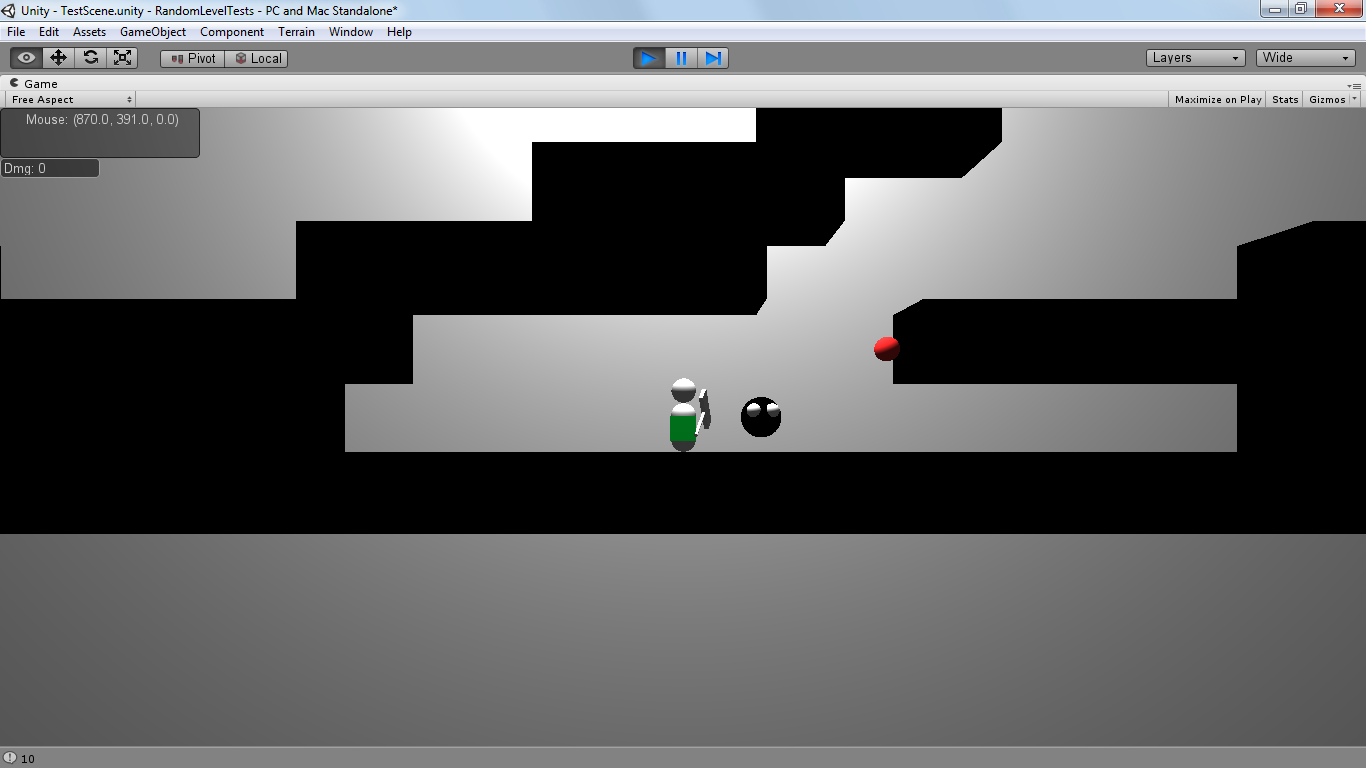
\includegraphics[width=5in]{Graphics/Pre_Hit.png}
\caption{Player prior to attacking the enemy.}
\label{PreHit}

\end{figure}

\begin{figure}[h!]

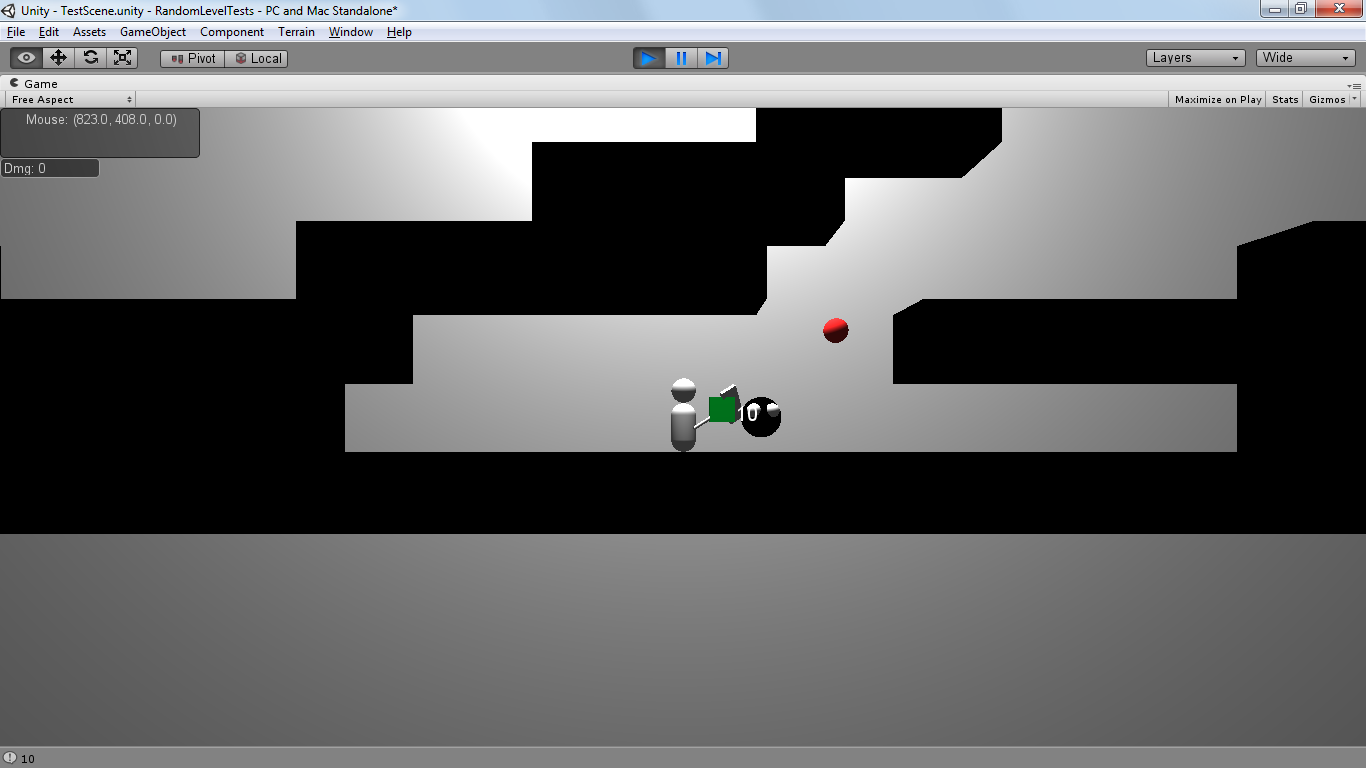
\includegraphics[width=5in]{Graphics/During_Hit.png}
\caption{Player while attacking the enemy.}
\label{DuringHit}

\end{figure}

The complete process looks something like this:
\begin{enumerate}

\item Hit box collides with enemy, collision handler is called.
\item An attack message with properties \{attack=20, isContact = false, element = ICE\} is sent to the enemy.
\item The entity processes the attack message, multiplying the damage by 2 (yielding 40) because of the ICE attribute.
\item The attack message is then passed off to the Stats object.  Because the ignoreDefense flag is set to false, the defense value (10) is subtracted from the damage value (yielding 30).  The final damage is subsequently subtracted from the HP value (yielding 70 HP).
\item The final damage value (30) is displayed on screen  above the enemy.

\end{enumerate}



\begin{figure}[htbp]
	%\makebox[\textwidth]{\hrulefill}{
	%\small
	\lstinputlisting[language=java, breaklines=true, numbers=left]{Code/collideHandler.cs}
	%\normalsize}
	\caption{The hitbox's collision handling method.}
	\label{CollideHandler}
\end{figure}

\begin{figure}[htbp]
	%\makebox[\textwidth]{\hrulefill}{
	%\small
	\lstinputlisting[language=java, breaklines=true, numbers=left]{Code/takedamage.cs}
	%\normalsize}
	\caption{The enemy's TakeDamage method.}
	\label{TakeDamage}
\end{figure}


\subsection{Graphics}

Despite having gameplay restricted along a 2D plane, the game's graphics will be entirely 3D.  Models and animations will be created using Blender and imported to Unity.  The technical aspects of the rendering will be handled by Unity's graphics engine.

\subsubsection{Unity Graphics Overview}

Being a multi-platform engine, the specifics of the graphics engine vary between platforms.  The two platforms we will be focusing on are what is referred to in the Unity documentation as "Desktop" platforms, which includes Windows PC and Mac systems.  The windows version of the rendering engine uses Direct3D, while OpenGL is used in the Mac version.  For desktop games, a wide variety of rendering options are available, including over 100 shaders, the ability to create custom CG and GLSL shaders, and many more.  Additionally, many rendering optimizations are present, such as deferred rendering and batching.

While the specifics of the rendering engine are much too complex to understand for such a small development team with limited time and resources, certain key details are revealed on Unity's website so that developers can optimize their graphics performance.  The most significant of these details as they apply to our game are those about optimizing meshes.  It is suggested that each mesh should be between 1500 and 4000 triangles, and that each should use a single material, as multi-material meshes are rendered once for each material attached to them.  We will attempt to follow these guidelines as closely as possible to optimize graphics performance.

Additionally, there are several emulation modes available with the Unity graphics engine, which can be used to test compatibility with older hardware.  Because we do not want our game to have high technical requirements, we will likely make use of this feature.

\subsubsection{Models and Animations}

As mentioned, Blender will be used to create models and animation.  The development team has experience with Blender, so there is an extremely low learning curve.  Additionally, Unity includes built-in support for importing Blender models and animations, further reducing the effort required to create 3D graphics.

Both Blender and Unity support skeletal animation systems, which further simplifies the task of animation.  The positions of bones can be keyframed in Blender to produce animations, and those animations will carry over to Unity when imported.  An issue that causes some concern is the absence of an inverse kinematics system in Unity, despite its availability in Blender.  Inverse kinematics solvers enable chains of bones (such as limbs) to be more easily animated.  However, by keyframing the position and rotation attributes of the bones controlled by inverse kinematics in Blender, and through use of animation blending, we should be able to accomplish most animation tasks.

Animation blending is also supported by both systems, which means that muiltiple animations can be combined in new and interesting ways.  One of the features this is used to implement is the player's directional attacking ability.  Figures \ref{ForwardHit}, \ref{UpHit} and \ref{DiagHit} show how this can be accomplished.  Only two animations have been defined manually - the forward hit and upward hit animations.  Attacks always occur in the direction of the mouse pointer.  In these cases, weights are assigned to the animations based on the angle between the player and the mouse pointer.  The upward hit is proportional to the sine (dy / hyp), and the forward hit is proportional to the cosine (dx / hyp).  Thus, when dx = 0, the sine is 1 and the cosine is 0, resulting in a complete upward hit.  When dy = 0, the cosine is 1, resulting in a complete forward hit.  For any angles in between, the weights are appropriately adjusted to combine the animations in the right proportions.

\begin{figure}[h!]

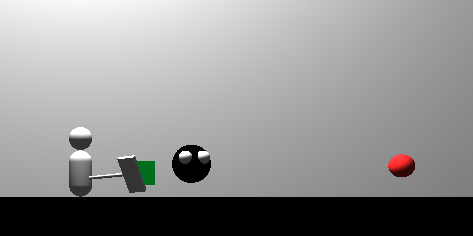
\includegraphics[width=5in]{Graphics/forwardHit.png}
\caption{The forward hit animation.}
\label{ForwardHit}

\end{figure}

\begin{figure}[h!]

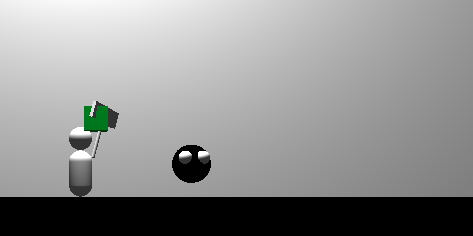
\includegraphics[width=5in]{Graphics/upHit.png}
\caption{The upward hit animation.}
\label{UpHit}

\end{figure}

\begin{figure}[h!]

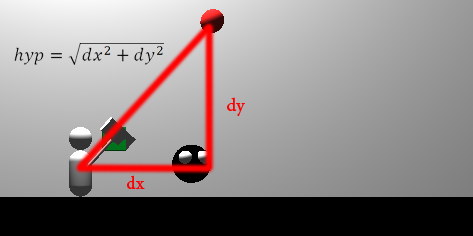
\includegraphics[width=5in]{Graphics/hitDiag.png}
\caption{The result of combined up and forward hit animations.}
\label{DiagHit}

\end{figure}

\subsection{Audio}

Unity's audio system is very easy to use and supports a number of different audio types.  Audio assets can be imported from .aif, .wav, .mp3, and .ogg formats.  When the assets are imported, they can be built into one of 2 formats: native (.wav) and compressed (using Ogg Vorbis compression).  Mono, stereo, and multi-channel audio (up to 8 channels) are also supported.

Unity also supports 3D sound, allowing audio sources to be placed at 3D coordinates in the game world.  AudioSource components are attached to game objects, and will produce sound at their location.  Many aspects of an AudioSource, such as reverberation and distance fall-off functions can be edited to suit the developer's needs.

\subsection{Artificial Intelligence}

In this game there will be different enemies with different attributes and qualities. Each enemy has a finite state machine which is managed by an EntityControl class. Each enemy class overrides this class to get his own special behaviour, attacks and qualities.

As said before enemies are similar to the player in a sense that they all have stats.  Inside of each entity controller there is a Stats object.   The functionality of the finite state machine model is outlined in section \ref{Architecture}.  In this section, the specifics of each enemy's finite state machine will be detailed.

\subsubsection{Description of Common States}
A number of states are shared among many of the enemies, and will have their own implementations in each EntityControl class.  However, the core of their functionality is the same.

\paragraph{Wander}
The start state for almost all enemies is wandering. In this state the entity moves around in random direction for a certain amount of time.  It changes the direction after time out and chooses another random direction.  For most enemies, this involves moving along the ground.  Floating enemies such as F. Headman and Shadowman may wander in any direction.

\paragraph{Close In}
In each update the enemy checks if the player is visible by ray casting.  If the player is seen, the state machine will typically transition to the close-in state, in which the player is pursued.  Pursuit stops when the player is in range, or when visibility is cut off.  If the entity faces an obstacle which hides the player, it will go back to the wandering state.

\paragraph{Attack}
If the enemy successfully gets in range of the player, it starts periodic attacks.  If the player gets out of the enemy’s range it will go back to the close-in state.

\paragraph{Dead}
In each update the enemy game stats will be checked to see if it is alive or not.  This means checking his HP level.  If HP equals zero the enemy is dead.  The dead state isn't shown in any of the diagrams but obviously in every update HP will be checked.  Zero HP will result in a transition between any of the active states and the Dead state.

\subsubsection{Enemy-specific Idiosyncracies}

\begin{figure}[h!]
{\scalefont{1.0}
% Graphic for TeX using PGF
% Title: C:\Users\Kaylen\CotWM\Doc\Graphics\wyrim.dia
% Creator: Dia v0.97.1
% CreationDate: Mon Mar 12 02:54:36 2012
% For: Kaylen
% \usepackage{tikz}
% The following commands are not supported in PSTricks at present
% We define them conditionally, so when they are implemented,
% this pgf file will use them.
\ifx\du\undefined
  \newlength{\du}
\fi
\setlength{\du}{15\unitlength}
\begin{tikzpicture}
\pgftransformxscale{0.526085}
\pgftransformyscale{-0.526085}
\definecolor{dialinecolor}{rgb}{0.000000, 0.000000, 0.000000}
\pgfsetstrokecolor{dialinecolor}
\definecolor{dialinecolor}{rgb}{1.000000, 1.000000, 1.000000}
\pgfsetfillcolor{dialinecolor}
\definecolor{dialinecolor}{rgb}{1.000000, 1.000000, 1.000000}
\pgfsetfillcolor{dialinecolor}
\pgfpathellipse{\pgfpoint{11.846634\du}{8.623322\du}}{\pgfpoint{4.553364\du}{0\du}}{\pgfpoint{0\du}{1.876682\du}}
\pgfusepath{fill}
\pgfsetlinewidth{0.100000\du}
\pgfsetdash{}{0pt}
\pgfsetdash{}{0pt}
\pgfsetmiterjoin
\definecolor{dialinecolor}{rgb}{0.000000, 0.000000, 0.000000}
\pgfsetstrokecolor{dialinecolor}
\pgfpathellipse{\pgfpoint{11.846634\du}{8.623322\du}}{\pgfpoint{4.553364\du}{0\du}}{\pgfpoint{0\du}{1.876682\du}}
\pgfusepath{stroke}
% setfont left to latex
\definecolor{dialinecolor}{rgb}{0.000000, 0.000000, 0.000000}
\pgfsetstrokecolor{dialinecolor}
\node at (11.846634\du,8.863322\du){wander};
\definecolor{dialinecolor}{rgb}{1.000000, 1.000000, 1.000000}
\pgfsetfillcolor{dialinecolor}
\pgfpathellipse{\pgfpoint{31.828364\du}{8.371682\du}}{\pgfpoint{4.553364\du}{0\du}}{\pgfpoint{0\du}{1.876682\du}}
\pgfusepath{fill}
\pgfsetlinewidth{0.100000\du}
\pgfsetdash{}{0pt}
\pgfsetdash{}{0pt}
\pgfsetmiterjoin
\definecolor{dialinecolor}{rgb}{0.000000, 0.000000, 0.000000}
\pgfsetstrokecolor{dialinecolor}
\pgfpathellipse{\pgfpoint{31.828364\du}{8.371682\du}}{\pgfpoint{4.553364\du}{0\du}}{\pgfpoint{0\du}{1.876682\du}}
\pgfusepath{stroke}
% setfont left to latex
\definecolor{dialinecolor}{rgb}{0.000000, 0.000000, 0.000000}
\pgfsetstrokecolor{dialinecolor}
\node at (31.828364\du,8.611682\du){sucking blood};
% setfont left to latex
\definecolor{dialinecolor}{rgb}{0.000000, 0.000000, 0.000000}
\pgfsetstrokecolor{dialinecolor}
\node[anchor=west] at (11.846600\du,8.623320\du){};
% setfont left to latex
\definecolor{dialinecolor}{rgb}{0.000000, 0.000000, 0.000000}
\pgfsetstrokecolor{dialinecolor}
\node[anchor=west] at (11.846600\du,8.623320\du){};
\pgfsetlinewidth{0.100000\du}
\pgfsetbuttcap
\pgfsetdash{}{0pt}
{
\definecolor{dialinecolor}{rgb}{0.000000, 0.000000, 0.000000}
\pgfsetfillcolor{dialinecolor}
% was here!!!
\pgfsetarrowsstart{latex}
\definecolor{dialinecolor}{rgb}{0.000000, 0.000000, 0.000000}
\pgfsetstrokecolor{dialinecolor}
\draw (27.621600\du,7.653510\du)--(15.400000\du,7.400000\du);
}
% setfont left to latex
\definecolor{dialinecolor}{rgb}{0.000000, 0.000000, 0.000000}
\pgfsetstrokecolor{dialinecolor}
\node at (21.510800\du,8.026750\du){touch player};
\end{tikzpicture}

}
\caption{A Wyrm's state machine.}
\label{FSMWyrm}

\end{figure}
\paragraph{Wyrm}
The Wyrms lack a close-in state.  Instead, they wander until they make contact with the player, at which point they latch onto the player and continue attacking.  Wyrms are not highly sophistocated enemies.  They have low HP and draw their strength from being in large groups.

\begin{figure}[h!]
{\scalefont{0.6}
\input{Graphics/F-Headman.tex}
}
\caption{F. Headman's state machine.}
\label{FSMFHead}
\end{figure}

\paragraph{F. Headman}
The F. Headman enemies follow the common states very closely.  Their attack involves spitting fire at the player.

\paragraph{Shadowman}
The Shadowman is very similar to F. Headman.  However, the attack is different.  When it comes into close range of the player, it opens its cloak and expands.  In this expanding state, it attempts to suck the player in.  If the player is sucked in, it is attacked and expelled.  If the player escapes, the Shadowman goes back to the wandering state.

\begin{figure}[h!]
{\scalefont{0.6}
% Graphic for TeX using PGF
% Title: C:\Users\Kaylen\CotWM\Doc\Graphics\SnowMan.dia
% Creator: Dia v0.97.1
% CreationDate: Mon Mar 12 10:51:53 2012
% For: Kaylen
% \usepackage{tikz}
% The following commands are not supported in PSTricks at present
% We define them conditionally, so when they are implemented,
% this pgf file will use them.
\ifx\du\undefined
  \newlength{\du}
\fi
\setlength{\du}{15\unitlength}
\begin{tikzpicture}
\pgftransformxscale{0.743267}
\pgftransformyscale{-0.743267}
\definecolor{dialinecolor}{rgb}{0.000000, 0.000000, 0.000000}
\pgfsetstrokecolor{dialinecolor}
\definecolor{dialinecolor}{rgb}{1.000000, 1.000000, 1.000000}
\pgfsetfillcolor{dialinecolor}
% setfont left to latex
\definecolor{dialinecolor}{rgb}{0.000000, 0.000000, 0.000000}
\pgfsetstrokecolor{dialinecolor}
\node[anchor=west] at (3.887500\du,16.647500\du){};
% setfont left to latex
\definecolor{dialinecolor}{rgb}{0.000000, 0.000000, 0.000000}
\pgfsetstrokecolor{dialinecolor}
\node[anchor=west] at (3.887500\du,16.647500\du){};
% setfont left to latex
\definecolor{dialinecolor}{rgb}{0.000000, 0.000000, 0.000000}
\pgfsetstrokecolor{dialinecolor}
\node[anchor=west] at (51.225000\du,5.297250\du){};
% setfont left to latex
\definecolor{dialinecolor}{rgb}{0.000000, 0.000000, 0.000000}
\pgfsetstrokecolor{dialinecolor}
\node[anchor=west] at (13.950000\du,7.790000\du){};
\definecolor{dialinecolor}{rgb}{1.000000, 1.000000, 1.000000}
\pgfsetfillcolor{dialinecolor}
\pgfpathellipse{\pgfpoint{13.303364\du}{13.006682\du}}{\pgfpoint{3.503364\du}{0\du}}{\pgfpoint{0\du}{1.776682\du}}
\pgfusepath{fill}
\pgfsetlinewidth{0.100000\du}
\pgfsetdash{}{0pt}
\pgfsetdash{}{0pt}
\pgfsetmiterjoin
\definecolor{dialinecolor}{rgb}{0.000000, 0.000000, 0.000000}
\pgfsetstrokecolor{dialinecolor}
\pgfpathellipse{\pgfpoint{13.303364\du}{13.006682\du}}{\pgfpoint{3.503364\du}{0\du}}{\pgfpoint{0\du}{1.776682\du}}
\pgfusepath{stroke}
% setfont left to latex
\definecolor{dialinecolor}{rgb}{0.000000, 0.000000, 0.000000}
\pgfsetstrokecolor{dialinecolor}
\node at (13.303364\du,13.246682\du){standing still};
\definecolor{dialinecolor}{rgb}{1.000000, 1.000000, 1.000000}
\pgfsetfillcolor{dialinecolor}
\pgfpathellipse{\pgfpoint{27.878364\du}{5.901682\du}}{\pgfpoint{3.503364\du}{0\du}}{\pgfpoint{0\du}{1.776682\du}}
\pgfusepath{fill}
\pgfsetlinewidth{0.100000\du}
\pgfsetdash{}{0pt}
\pgfsetdash{}{0pt}
\pgfsetmiterjoin
\definecolor{dialinecolor}{rgb}{0.000000, 0.000000, 0.000000}
\pgfsetstrokecolor{dialinecolor}
\pgfpathellipse{\pgfpoint{27.878364\du}{5.901682\du}}{\pgfpoint{3.503364\du}{0\du}}{\pgfpoint{0\du}{1.776682\du}}
\pgfusepath{stroke}
% setfont left to latex
\definecolor{dialinecolor}{rgb}{0.000000, 0.000000, 0.000000}
\pgfsetstrokecolor{dialinecolor}
\node at (27.878364\du,6.141682\du){snow ball attack};
\definecolor{dialinecolor}{rgb}{1.000000, 1.000000, 1.000000}
\pgfsetfillcolor{dialinecolor}
\pgfpathellipse{\pgfpoint{28.753364\du}{13.246682\du}}{\pgfpoint{3.503364\du}{0\du}}{\pgfpoint{0\du}{1.776682\du}}
\pgfusepath{fill}
\pgfsetlinewidth{0.100000\du}
\pgfsetdash{}{0pt}
\pgfsetdash{}{0pt}
\pgfsetmiterjoin
\definecolor{dialinecolor}{rgb}{0.000000, 0.000000, 0.000000}
\pgfsetstrokecolor{dialinecolor}
\pgfpathellipse{\pgfpoint{28.753364\du}{13.246682\du}}{\pgfpoint{3.503364\du}{0\du}}{\pgfpoint{0\du}{1.776682\du}}
\pgfusepath{stroke}
% setfont left to latex
\definecolor{dialinecolor}{rgb}{0.000000, 0.000000, 0.000000}
\pgfsetstrokecolor{dialinecolor}
\node at (28.753364\du,13.486682\du){attacking};
\definecolor{dialinecolor}{rgb}{1.000000, 1.000000, 1.000000}
\pgfsetfillcolor{dialinecolor}
\pgfpathellipse{\pgfpoint{29.350000\du}{20.690000\du}}{\pgfpoint{3.550000\du}{0\du}}{\pgfpoint{0\du}{1.700000\du}}
\pgfusepath{fill}
\pgfsetlinewidth{0.100000\du}
\pgfsetdash{}{0pt}
\pgfsetdash{}{0pt}
\pgfsetmiterjoin
\definecolor{dialinecolor}{rgb}{0.000000, 0.000000, 0.000000}
\pgfsetstrokecolor{dialinecolor}
\pgfpathellipse{\pgfpoint{29.350000\du}{20.690000\du}}{\pgfpoint{3.550000\du}{0\du}}{\pgfpoint{0\du}{1.700000\du}}
\pgfusepath{stroke}
% setfont left to latex
\definecolor{dialinecolor}{rgb}{0.000000, 0.000000, 0.000000}
\pgfsetstrokecolor{dialinecolor}
\node at (29.350000\du,20.930000\du){ice breath};
\definecolor{dialinecolor}{rgb}{1.000000, 1.000000, 1.000000}
\pgfsetfillcolor{dialinecolor}
\pgfpathellipse{\pgfpoint{41.653364\du}{13.286682\du}}{\pgfpoint{3.503364\du}{0\du}}{\pgfpoint{0\du}{1.776682\du}}
\pgfusepath{fill}
\pgfsetlinewidth{0.100000\du}
\pgfsetdash{}{0pt}
\pgfsetdash{}{0pt}
\pgfsetmiterjoin
\definecolor{dialinecolor}{rgb}{0.000000, 0.000000, 0.000000}
\pgfsetstrokecolor{dialinecolor}
\pgfpathellipse{\pgfpoint{41.653364\du}{13.286682\du}}{\pgfpoint{3.503364\du}{0\du}}{\pgfpoint{0\du}{1.776682\du}}
\pgfusepath{stroke}
% setfont left to latex
\definecolor{dialinecolor}{rgb}{0.000000, 0.000000, 0.000000}
\pgfsetstrokecolor{dialinecolor}
\node at (41.653364\du,13.526682\du){avalanche};
\pgfsetlinewidth{0.100000\du}
\pgfsetdash{}{0pt}
\pgfsetdash{}{0pt}
\pgfsetbuttcap
{
\definecolor{dialinecolor}{rgb}{0.000000, 0.000000, 0.000000}
\pgfsetfillcolor{dialinecolor}
% was here!!!
\pgfsetarrowsend{stealth}
\definecolor{dialinecolor}{rgb}{0.000000, 0.000000, 0.000000}
\pgfsetstrokecolor{dialinecolor}
\pgfpathmoveto{\pgfpoint{16.276959\du}{13.997111\du}}
\pgfpatharc{104}{76}{18.140269\du and 18.140269\du}
\pgfusepath{stroke}
}
\pgfsetlinewidth{0.100000\du}
\pgfsetdash{}{0pt}
\pgfsetdash{}{0pt}
\pgfsetbuttcap
{
\definecolor{dialinecolor}{rgb}{0.000000, 0.000000, 0.000000}
\pgfsetfillcolor{dialinecolor}
% was here!!!
\pgfsetarrowsend{stealth}
\definecolor{dialinecolor}{rgb}{0.000000, 0.000000, 0.000000}
\pgfsetstrokecolor{dialinecolor}
\pgfpathmoveto{\pgfpoint{25.869104\du}{12.187455\du}}
\pgfpatharc{286}{258}{19.651786\du and 19.651786\du}
\pgfusepath{stroke}
}
\pgfsetlinewidth{0.100000\du}
\pgfsetdash{}{0pt}
\pgfsetdash{}{0pt}
\pgfsetbuttcap
{
\definecolor{dialinecolor}{rgb}{0.000000, 0.000000, 0.000000}
\pgfsetfillcolor{dialinecolor}
% was here!!!
\pgfsetarrowsend{stealth}
\definecolor{dialinecolor}{rgb}{0.000000, 0.000000, 0.000000}
\pgfsetstrokecolor{dialinecolor}
\pgfpathmoveto{\pgfpoint{26.693830\du}{7.619949\du}}
\pgfpatharc{202}{151}{4.652364\du and 4.652364\du}
\pgfusepath{stroke}
}
\pgfsetlinewidth{0.100000\du}
\pgfsetdash{}{0pt}
\pgfsetdash{}{0pt}
\pgfsetbuttcap
{
\definecolor{dialinecolor}{rgb}{0.000000, 0.000000, 0.000000}
\pgfsetfillcolor{dialinecolor}
% was here!!!
\pgfsetarrowsend{stealth}
\definecolor{dialinecolor}{rgb}{0.000000, 0.000000, 0.000000}
\pgfsetstrokecolor{dialinecolor}
\pgfpathmoveto{\pgfpoint{30.093817\du}{11.605341\du}}
\pgfpatharc{53}{-52}{2.565736\du and 2.565736\du}
\pgfusepath{stroke}
}
\pgfsetlinewidth{0.100000\du}
\pgfsetdash{}{0pt}
\pgfsetdash{}{0pt}
\pgfsetbuttcap
{
\definecolor{dialinecolor}{rgb}{0.000000, 0.000000, 0.000000}
\pgfsetfillcolor{dialinecolor}
% was here!!!
\pgfsetarrowsend{stealth}
\definecolor{dialinecolor}{rgb}{0.000000, 0.000000, 0.000000}
\pgfsetstrokecolor{dialinecolor}
\pgfpathmoveto{\pgfpoint{31.989818\du}{13.926389\du}}
\pgfpatharc{127}{55}{5.166862\du and 5.166862\du}
\pgfusepath{stroke}
}
\pgfsetlinewidth{0.100000\du}
\pgfsetdash{}{0pt}
\pgfsetdash{}{0pt}
\pgfsetbuttcap
{
\definecolor{dialinecolor}{rgb}{0.000000, 0.000000, 0.000000}
\pgfsetfillcolor{dialinecolor}
% was here!!!
\pgfsetarrowsend{stealth}
\definecolor{dialinecolor}{rgb}{0.000000, 0.000000, 0.000000}
\pgfsetstrokecolor{dialinecolor}
\pgfpathmoveto{\pgfpoint{38.300062\du}{12.440047\du}}
\pgfpatharc{307}{234}{5.000000\du and 5.000000\du}
\pgfusepath{stroke}
}
\pgfsetlinewidth{0.100000\du}
\pgfsetdash{}{0pt}
\pgfsetdash{}{0pt}
\pgfsetbuttcap
{
\definecolor{dialinecolor}{rgb}{0.000000, 0.000000, 0.000000}
\pgfsetfillcolor{dialinecolor}
% was here!!!
\pgfsetarrowsend{stealth}
\definecolor{dialinecolor}{rgb}{0.000000, 0.000000, 0.000000}
\pgfsetstrokecolor{dialinecolor}
\pgfpathmoveto{\pgfpoint{30.349826\du}{18.890107\du}}
\pgfpatharc{59}{-52}{2.310000\du and 2.310000\du}
\pgfusepath{stroke}
}
\pgfsetlinewidth{0.100000\du}
\pgfsetdash{}{0pt}
\pgfsetdash{}{0pt}
\pgfsetbuttcap
{
\definecolor{dialinecolor}{rgb}{0.000000, 0.000000, 0.000000}
\pgfsetfillcolor{dialinecolor}
% was here!!!
\pgfsetarrowsend{stealth}
\definecolor{dialinecolor}{rgb}{0.000000, 0.000000, 0.000000}
\pgfsetstrokecolor{dialinecolor}
\pgfpathmoveto{\pgfpoint{27.412775\du}{14.888040\du}}
\pgfpatharc{232}{127}{2.553189\du and 2.553189\du}
\pgfusepath{stroke}
}
% setfont left to latex
\definecolor{dialinecolor}{rgb}{0.000000, 0.000000, 0.000000}
\pgfsetstrokecolor{dialinecolor}
\node[anchor=west] at (27.878400\du,5.901680\du){};
% setfont left to latex
\definecolor{dialinecolor}{rgb}{0.000000, 0.000000, 0.000000}
\pgfsetstrokecolor{dialinecolor}
\node[anchor=west] at (19.800000\du,10.675000\du){};
% setfont left to latex
\definecolor{dialinecolor}{rgb}{0.000000, 0.000000, 0.000000}
\pgfsetstrokecolor{dialinecolor}
\node[anchor=west] at (19.450000\du,11.075000\du){};
% setfont left to latex
\definecolor{dialinecolor}{rgb}{0.000000, 0.000000, 0.000000}
\pgfsetstrokecolor{dialinecolor}
\node[anchor=west] at (20.500000\du,14.375000\du){};
% setfont left to latex
\definecolor{dialinecolor}{rgb}{0.000000, 0.000000, 0.000000}
\pgfsetstrokecolor{dialinecolor}
\node[anchor=west] at (17.750000\du,14.875000\du){player enters the room};
% setfont left to latex
\definecolor{dialinecolor}{rgb}{0.000000, 0.000000, 0.000000}
\pgfsetstrokecolor{dialinecolor}
\node[anchor=west] at (22.850000\du,10.975000\du){};
% setfont left to latex
\definecolor{dialinecolor}{rgb}{0.000000, 0.000000, 0.000000}
\pgfsetstrokecolor{dialinecolor}
\node[anchor=west] at (17.750000\du,11.225000\du){player lefts the room};
% setfont left to latex
\definecolor{dialinecolor}{rgb}{0.000000, 0.000000, 0.000000}
\pgfsetstrokecolor{dialinecolor}
\node[anchor=west] at (30.250000\du,8.525000\du){};
% setfont left to latex
\definecolor{dialinecolor}{rgb}{0.000000, 0.000000, 0.000000}
\pgfsetstrokecolor{dialinecolor}
\node[anchor=west] at (30.250000\du,9.675000\du){attack time out};
% setfont left to latex
\definecolor{dialinecolor}{rgb}{0.000000, 0.000000, 0.000000}
\pgfsetstrokecolor{dialinecolor}
\node[anchor=west] at (34.100000\du,14.675000\du){};
% setfont left to latex
\definecolor{dialinecolor}{rgb}{0.000000, 0.000000, 0.000000}
\pgfsetstrokecolor{dialinecolor}
\node[anchor=west] at (33.900000\du,14.975000\du){};
% setfont left to latex
\definecolor{dialinecolor}{rgb}{0.000000, 0.000000, 0.000000}
\pgfsetstrokecolor{dialinecolor}
\node[anchor=west] at (33.900000\du,15.275000\du){attack time out};
% setfont left to latex
\definecolor{dialinecolor}{rgb}{0.000000, 0.000000, 0.000000}
\pgfsetstrokecolor{dialinecolor}
\node[anchor=west] at (24.100000\du,17.325000\du){attack time out};
% setfont left to latex
\definecolor{dialinecolor}{rgb}{0.000000, 0.000000, 0.000000}
\pgfsetstrokecolor{dialinecolor}
\node[anchor=west] at (24.000000\du,8.175000\du){};
% setfont left to latex
\definecolor{dialinecolor}{rgb}{0.000000, 0.000000, 0.000000}
\pgfsetstrokecolor{dialinecolor}
\node[anchor=west] at (24.100000\du,8.375000\du){attack finished};
% setfont left to latex
\definecolor{dialinecolor}{rgb}{0.000000, 0.000000, 0.000000}
\pgfsetstrokecolor{dialinecolor}
\node[anchor=west] at (34.350000\du,11.425000\du){attack finished};
% setfont left to latex
\definecolor{dialinecolor}{rgb}{0.000000, 0.000000, 0.000000}
\pgfsetstrokecolor{dialinecolor}
\node[anchor=west] at (31.700000\du,16.925000\du){attack finished};
\end{tikzpicture}

}
\caption{Abominable Snowman's state machine.}
\label{FSMSnowman}
\end{figure}

\paragraph{Abominable Snowman}
The abominable snowman does not have a wander state, as it is a stationary enemy that relies primarily on ranged attacks.  It automatically enters the attacking state from the idle state when the player enters the room, at which point it randomly selects an attack to use after a certain time-out.  It continues this process indefinitely after the attack is complete.  It has three options for attacks - throwing a snowball, using ice breath, and causing an avalanche from the ceiling of the room.

\begin{figure}[h!]
{\scalefont{0.6}
% Graphic for TeX using PGF
% Title: C:\Users\Kaylen\CotWM\Doc\Graphics\khoak.dia
% Creator: Dia v0.97.1
% CreationDate: Mon Mar 12 02:57:35 2012
% For: Kaylen
% \usepackage{tikz}
% The following commands are not supported in PSTricks at present
% We define them conditionally, so when they are implemented,
% this pgf file will use them.
\ifx\du\undefined
  \newlength{\du}
\fi
\setlength{\du}{15\unitlength}
\begin{tikzpicture}
\pgftransformxscale{0.726574}
\pgftransformyscale{-0.726574}
\definecolor{dialinecolor}{rgb}{0.000000, 0.000000, 0.000000}
\pgfsetstrokecolor{dialinecolor}
\definecolor{dialinecolor}{rgb}{1.000000, 1.000000, 1.000000}
\pgfsetfillcolor{dialinecolor}
\definecolor{dialinecolor}{rgb}{1.000000, 1.000000, 1.000000}
\pgfsetfillcolor{dialinecolor}
\pgfpathellipse{\pgfpoint{32.437500\du}{9.305865\du}}{\pgfpoint{3.837500\du}{0\du}}{\pgfpoint{0\du}{1.807495\du}}
\pgfusepath{fill}
\pgfsetlinewidth{0.100000\du}
\pgfsetdash{}{0pt}
\pgfsetdash{}{0pt}
\pgfsetmiterjoin
\definecolor{dialinecolor}{rgb}{0.000000, 0.000000, 0.000000}
\pgfsetstrokecolor{dialinecolor}
\pgfpathellipse{\pgfpoint{32.437500\du}{9.305865\du}}{\pgfpoint{3.837500\du}{0\du}}{\pgfpoint{0\du}{1.807495\du}}
\pgfusepath{stroke}
% setfont left to latex
\definecolor{dialinecolor}{rgb}{0.000000, 0.000000, 0.000000}
\pgfsetstrokecolor{dialinecolor}
\node at (32.437500\du,9.545865\du){close in };
\definecolor{dialinecolor}{rgb}{1.000000, 1.000000, 1.000000}
\pgfsetfillcolor{dialinecolor}
\pgfpathellipse{\pgfpoint{19.350000\du}{9.303365\du}}{\pgfpoint{3.525000\du}{0\du}}{\pgfpoint{0\du}{1.754995\du}}
\pgfusepath{fill}
\pgfsetlinewidth{0.100000\du}
\pgfsetdash{}{0pt}
\pgfsetdash{}{0pt}
\pgfsetmiterjoin
\definecolor{dialinecolor}{rgb}{0.000000, 0.000000, 0.000000}
\pgfsetstrokecolor{dialinecolor}
\pgfpathellipse{\pgfpoint{19.350000\du}{9.303365\du}}{\pgfpoint{3.525000\du}{0\du}}{\pgfpoint{0\du}{1.754995\du}}
\pgfusepath{stroke}
% setfont left to latex
\definecolor{dialinecolor}{rgb}{0.000000, 0.000000, 0.000000}
\pgfsetstrokecolor{dialinecolor}
\node at (19.350000\du,9.543365\du){wandering};
\definecolor{dialinecolor}{rgb}{1.000000, 1.000000, 1.000000}
\pgfsetfillcolor{dialinecolor}
\pgfpathellipse{\pgfpoint{32.600000\du}{17.321682\du}}{\pgfpoint{3.925000\du}{0\du}}{\pgfpoint{0\du}{1.776682\du}}
\pgfusepath{fill}
\pgfsetlinewidth{0.100000\du}
\pgfsetdash{}{0pt}
\pgfsetdash{}{0pt}
\pgfsetmiterjoin
\definecolor{dialinecolor}{rgb}{0.000000, 0.000000, 0.000000}
\pgfsetstrokecolor{dialinecolor}
\pgfpathellipse{\pgfpoint{32.600000\du}{17.321682\du}}{\pgfpoint{3.925000\du}{0\du}}{\pgfpoint{0\du}{1.776682\du}}
\pgfusepath{stroke}
% setfont left to latex
\definecolor{dialinecolor}{rgb}{0.000000, 0.000000, 0.000000}
\pgfsetstrokecolor{dialinecolor}
\node at (32.600000\du,17.561682\du){attacking};
% setfont left to latex
\definecolor{dialinecolor}{rgb}{0.000000, 0.000000, 0.000000}
\pgfsetstrokecolor{dialinecolor}
\node[anchor=west] at (19.350000\du,9.303370\du){};
% setfont left to latex
\definecolor{dialinecolor}{rgb}{0.000000, 0.000000, 0.000000}
\pgfsetstrokecolor{dialinecolor}
\node[anchor=west] at (32.437500\du,9.305870\du){};
% setfont left to latex
\definecolor{dialinecolor}{rgb}{0.000000, 0.000000, 0.000000}
\pgfsetstrokecolor{dialinecolor}
\node[anchor=west] at (32.437500\du,9.305870\du){};
% setfont left to latex
\definecolor{dialinecolor}{rgb}{0.000000, 0.000000, 0.000000}
\pgfsetstrokecolor{dialinecolor}
\node[anchor=west] at (32.600000\du,17.321700\du){};
\pgfsetlinewidth{0.100000\du}
\pgfsetbuttcap
\pgfsetdash{}{0pt}
{
\definecolor{dialinecolor}{rgb}{0.000000, 0.000000, 0.000000}
\pgfsetfillcolor{dialinecolor}
% was here!!!
\pgfsetarrowsstart{latex}
\definecolor{dialinecolor}{rgb}{0.000000, 0.000000, 0.000000}
\pgfsetstrokecolor{dialinecolor}
\draw (28.525000\du,9.248370\du)--(22.875000\du,9.303370\du);
}
% setfont left to latex
\definecolor{dialinecolor}{rgb}{0.000000, 0.000000, 0.000000}
\pgfsetstrokecolor{dialinecolor}
\node at (25.700000\du,9.775870\du){see player};
\pgfsetlinewidth{0.100000\du}
\pgfsetbuttcap
\pgfsetdash{}{0pt}
{
\definecolor{dialinecolor}{rgb}{0.000000, 0.000000, 0.000000}
\pgfsetfillcolor{dialinecolor}
% was here!!!
\pgfsetarrowsstart{latex}
\definecolor{dialinecolor}{rgb}{0.000000, 0.000000, 0.000000}
\pgfsetstrokecolor{dialinecolor}
\draw (31.125000\du,15.298400\du)--(30.969000\du,10.975800\du);
}
% setfont left to latex
\definecolor{dialinecolor}{rgb}{0.000000, 0.000000, 0.000000}
\pgfsetstrokecolor{dialinecolor}
\node at (31.047000\du,13.637100\du){in range};
\pgfsetlinewidth{0.100000\du}
\pgfsetbuttcap
\pgfsetdash{}{0pt}
{
\definecolor{dialinecolor}{rgb}{0.000000, 0.000000, 0.000000}
\pgfsetfillcolor{dialinecolor}
% was here!!!
\pgfsetarrowsstart{latex}
\definecolor{dialinecolor}{rgb}{0.000000, 0.000000, 0.000000}
\pgfsetstrokecolor{dialinecolor}
\draw (35.106000\du,10.825800\du)--(35.225000\du,15.848400\du);
}
% setfont left to latex
\definecolor{dialinecolor}{rgb}{0.000000, 0.000000, 0.000000}
\pgfsetstrokecolor{dialinecolor}
\node at (35.165500\du,13.837100\du){out of range};
\pgfsetlinewidth{0.100000\du}
\pgfsetdash{}{0pt}
\pgfsetdash{}{0pt}
\pgfsetbuttcap
{
\definecolor{dialinecolor}{rgb}{0.000000, 0.000000, 0.000000}
\pgfsetfillcolor{dialinecolor}
% was here!!!
\pgfsetarrowsend{stealth}
\definecolor{dialinecolor}{rgb}{0.000000, 0.000000, 0.000000}
\pgfsetstrokecolor{dialinecolor}
\pgfpathmoveto{\pgfpoint{28.575038\du}{16.948419\du}}
\pgfpatharc{298}{-5}{2.317767\du and 2.317767\du}
\pgfusepath{stroke}
}
% setfont left to latex
\definecolor{dialinecolor}{rgb}{0.000000, 0.000000, 0.000000}
\pgfsetstrokecolor{dialinecolor}
\node[anchor=west] at (24.225000\du,18.898400\du){smack the player};
\end{tikzpicture}

}
\caption{Shoggoth's state machine.}
\label{FSMShoggoth}
\end{figure}

\paragraph{Shoggoth}
The shoggoths follow the common states very closely.  Its attack involves hititng the player with its tentacle, which sends the player flying.

\begin{figure}[h!]
{\scalefont{0.8}
\input{Graphics/boss.tex}
}
\caption{Xl'Grhthbtrg's state machine.}
\label{FSMBoss}
\end{figure}

\paragraph{Xl'Grhthbtrg}
Xl'Grhthbtrg acts similar to the abominable snowman.  Because it is a boss, it will be the only enemy in the room with the player during the battle.  The only difference with the snowman is in the behaviour associated with the attacks themselves.  It has three options for attacks - moving around while flailing tentacles, firing lasers from its tentacles, or filling the screen with "darkness", which stuns the player momentarily.

\subsection{Physics}

A physics engine is provided by default with Unity.  Although our game will not make heavy use of the physics engine, it is important for handling collision detection.  Unity provides a variety of basic collider components which can be attached to game objects.  Among these are primitives such as cubes, spheres, and capsules.  Colliders can be set as triggers, which enables them to detect collisions with other objects, but not affect those objects in any way (i.e. they can pass through other objects).  The extent to which the physics system is used in our game will be primarily for collision detection and response, which can be easily accomplished through collision event handlers (see Fig. \ref{CollideHandler}).

\subsection{Game Objects and Logic}

\subsubsection{Gameplay Overview}

Gameplay is restricted along the 2-dimensional XY plane, although the graphics are rendered in 3D.  The basic player actions can be classified as moving, attacking, and jumping.  There are several extensions of these actions that will be further elaborated upon in the Abilities section.

Levels will be randomly generated, and will consist of a 2-dimensional grid of cubes, some of which may be empty.  The non-empty cubes will consist of either snow or rock.  Attacking cubes made of snow will allow the player to destroy them and progress further in the game.

As the player explores the game world and defeats enemies, they will gain experience points.  The number of points gained is specific to the enemy type (see section \ref{StatsSection} for more details).

\subsubsection{Player and Enemy Attirbutes}

Players and enemies share certain attributes that determine how they act in combat.  The specific rules of combat are detailed in section \ref{CombatMechanics}.

\begin{description}

\item[HP]
Determines how much damage an entity can take before it is destroyed.  In the case of the player, HP is displayed in a number of discrete blocks.  Each consists of 100 HP.  (Similar to the energy tanks of the Metroid series.)

\item[MP]
Depleted when the player uses special abilities.  MP is also displayed as a number of discrete blocks, similar to HP.

\item[Attack]
The amount of damage dealt by an attack.

\item[Defense]
Resistance to attacks.

\item[Speed]
Affects movement and attack speed.

\end{description}

\label{CombatMechanics}
\subsubsection{Combat Mechanics}

When an attack connects with an entity, the attack attempts to remove HP equal to its power.  Before that damage is applied, the entity's defense value is subtracted.  The resulting value is clamped to a minimum of 1 HP of damage.  The total HP of any entity is clamped to a minimum of 0 and a maximum of their max HP value.

In addition to damage values, attacks can have elemental attributes.  Currently, the only three element types are fire, ice, and lightning.  Elemental attributes may have different effects on enemies, depending on how that enemy handles damage.

\label{AbilitiesSection}
\subsubsection{Abilities}
(Abilities that must be obtained after beginning the game are indicated by *.)

\begin{description}

\item[Moving]

Using directional keys (A and D by default), the player can move left and right.  The direction the player faces is determined by the direction of the mouse pointer from the player, not the direction of movement.

\item[Jumping]

Jumping is by default accomplished with the Space key.  Holding the jump key longer results in a higher jump.  The trajectory can be controlled in midair by using the directional keys.

\item[Crouching]

Using the down button (S by default), the player can crouch in order to avoid enemy attacks.  They are still able to attack in this state.

\item[High Jump]

If the player hits the jump key when crouched, a high jump will be executed.  This will allow the player to reach high areas.

\item[Wall Jumping]

A wall-jump ability is also available.  The ability can be used repeatedly in order to ascend walls.

\item[Attacking and Digging]

The standard attack is a simple slash with the snow shovel.  This will remain the same regardless of the level of the player, although the attack power may increase.  Standard attacks can be aimed in any direction, according to the position of the mouse cursor.

If the attack hits a cube of snow, it will be destroyed.

\item[Special Abilities*]

A number of special abilities will be available to the player.  They will be able to use them if they acquire them through use of the level-up pentagram.  The abilities are listed below.

\begin{description}

\item[Lightning Bolt*]

A bolt of lightning is fired in the direction of the cursor.  Lightning elemental attack.

\item[Flame Strike*]

A powerful slash with the shovel, but the shovel is covered in flame.  This results in greater damage and an increased area of effect.  Fire elemental attack.

\item[Ice Shield*]

A temporary shield of ice is generated around the player, stopping projectiles and damaging any enemies that come into contact with it.  Ice elemental attack.

\item[Heal*]

A special ability that allows the player to recover HP without using obtaining a health powerup.

\item[Dash*]

Allows quick, short bursts of movement.  Ideal for fast motion and evasion of enemies.  The player can dash both forwards or backwards.  The default dash keys are Q and E, used for left and right dashes respectively.

\end{description}

\end{description}

\subsubsection{Items}

Only two types of items are available to the player, and are randomly dropped by enemies.

\paragraph{HP Up}
This item heals one tank of HP.

\paragraph{MP Up}
This item heals one tank of MP.

\subsubsection{Enemies}

See section the image files included with the electronic submission for concept art.

\paragraph{Wyrm}
Millenia of exposure to the black Majyyks of the cursed glacier have turned worms into Wyrms!  They have little wings and sharp teeth and are scary now!  Watch out for their blood sucking attack.  It will suck your blood!

\paragraph{F. Headman}
Question 1: Does the F stand for Floating or Flaming?  Question 2: Does it really matter?  F. Headman is one of a decapitated horde of fire-breathing black metal singers cursed to float around and breathe fire for eternity.... which is not really a curse because it’s totally awesome!  Anyway, he can shoot fire at you, so watch it!

\paragraph{Shadowman}
A cursed soul destined to wander the bowels of the earth forever in search of flesh to satisfy its hunger.  He’s a robe hooded guy with skeleton arms or something.  He may seem fairly harmless, but he will open his robe to suck you in, so watch out!

\paragraph{Abominable Snowman}
Wow, look at this guy.  He has a knife for a nose!  That is not a carrot.  THAT IS WHAT MUTILATES CARROTS!  Just like this guy will mutilate YOU!

\paragraph{Shoggoth}
“It was a terrible, indescribable thing vaster than any subway train—a shapeless congeries of protoplasmic bubbles, faintly self-luminous, and with myriads of temporary eyes forming and un-forming as pustules of greenish light all over the tunnel-filling front that bore down upon us.”

These were the last words of HP Lovecraft before he was eaten by one of these bad boys.  You don’t want to get in their way.  They’ll form an un-form pustules of PAIN on the inside of your BRAIN!



\paragraph{Xl'Grhthbtrg}
The power of Xl'grhthlbtrg is not one that can be known by the simple minds of men, for his very existence is drawn from the blackest voids beyond the abominable stars. There he beholds the unspeakable creations of the Nameless One and screams his master's dark will across the cosmos.

Also, he’s the final boss of level 1.  You’d think that with all those cosmic powers, he’d be able to land a better gig.  Guess not!

%Because this 

\subsubsection{Levels}

Levels are randomly generated with every new game.  Level generation begins with the construction of a random maze, which is then processed to produce a complete level.  Enemies are then added to the level.  Level generation follows a three-step process, which is outlined here.

\paragraph{Maze Generation}
A maze generation algorithm called the Growing Tree algorithm is first initialized with a random seed, and then proceeds to generate a maze.  This maze generation algorithm ensures the creation of a maze with no loops.  That is, there is only one path between any two empty squares.  An example of such a maze can be seen in figure \ref{TextMaze}.  In this figure, X's represent walls, while periods represent empty spaces.

\begin{figure}[htbp]
	\verbatiminput{Code/mazetext.txt}
	\caption{A maze generated with the Growing Tree algorithm.}
	\label{TextMaze}
\end{figure}

\paragraph{Room Processing}
Once the maze is created, it is converted into a level.  This is done by replacing each empty square with a randomly selected Room type.  Room types are visible in section \ref{RoomAndEnemy}.  Once the rooms are in place, a second pass over the grid checks for adjacencies between rooms, and replaces the walls, ceiling, or floor with snow in order to allow the player to pass between adjacent rooms.

\begin{figure}[h!]

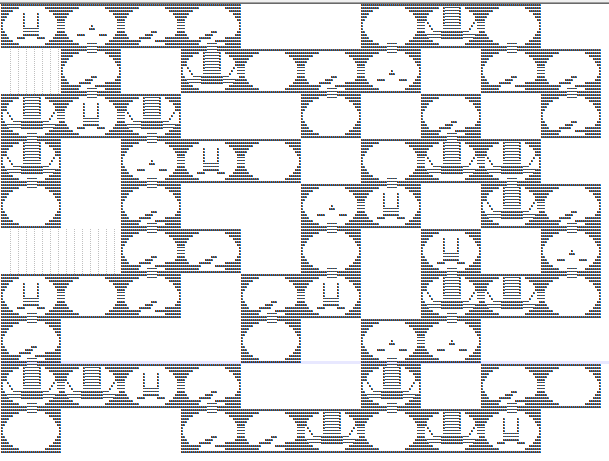
\includegraphics[width=5in]{Graphics/textmaze.png}
\caption{A fully-generated level.  Individual characters are not visible, as the image is zoomed-out.}
\label{TextLevel}

\end{figure}

\paragraph{Enemy Placement}
The third step involves placing enemies in the rooms.  For each room type, a number of enemy configurations are available.  These configurations are visible in section \ref{RoomAndEnemy}.  For each room, one of these configurations will be selected at random.  One exception to this rule is the boss room, which may only appear once per level.

\subsubsection{Gaining Experience and Abilities}

Increasing player stats and gaining abilities is achieved through use of the level-up pentagram.  The level-up pentagram (fig. \ref{Pentagram}) can be accessed through the status menu by pressing tab on the game screen.  It enables customization and specialization of stats and abilities, allowing different play experiences for different play-throughs of the game.

As the player defeats enemies, they gain experience points.  When enough experience is acquired to advance to the next level, the player gains a level-up point (see figure \ref{LevelupStats}).  Level-up points may be used to activate nodes on the level-up pentagram.  A node may only be activated if an adjacent node is also activated.  A special case is the first level-up, in which the player chooses one of the nodes on the inner pentagram.

\begin{figure}[h!]

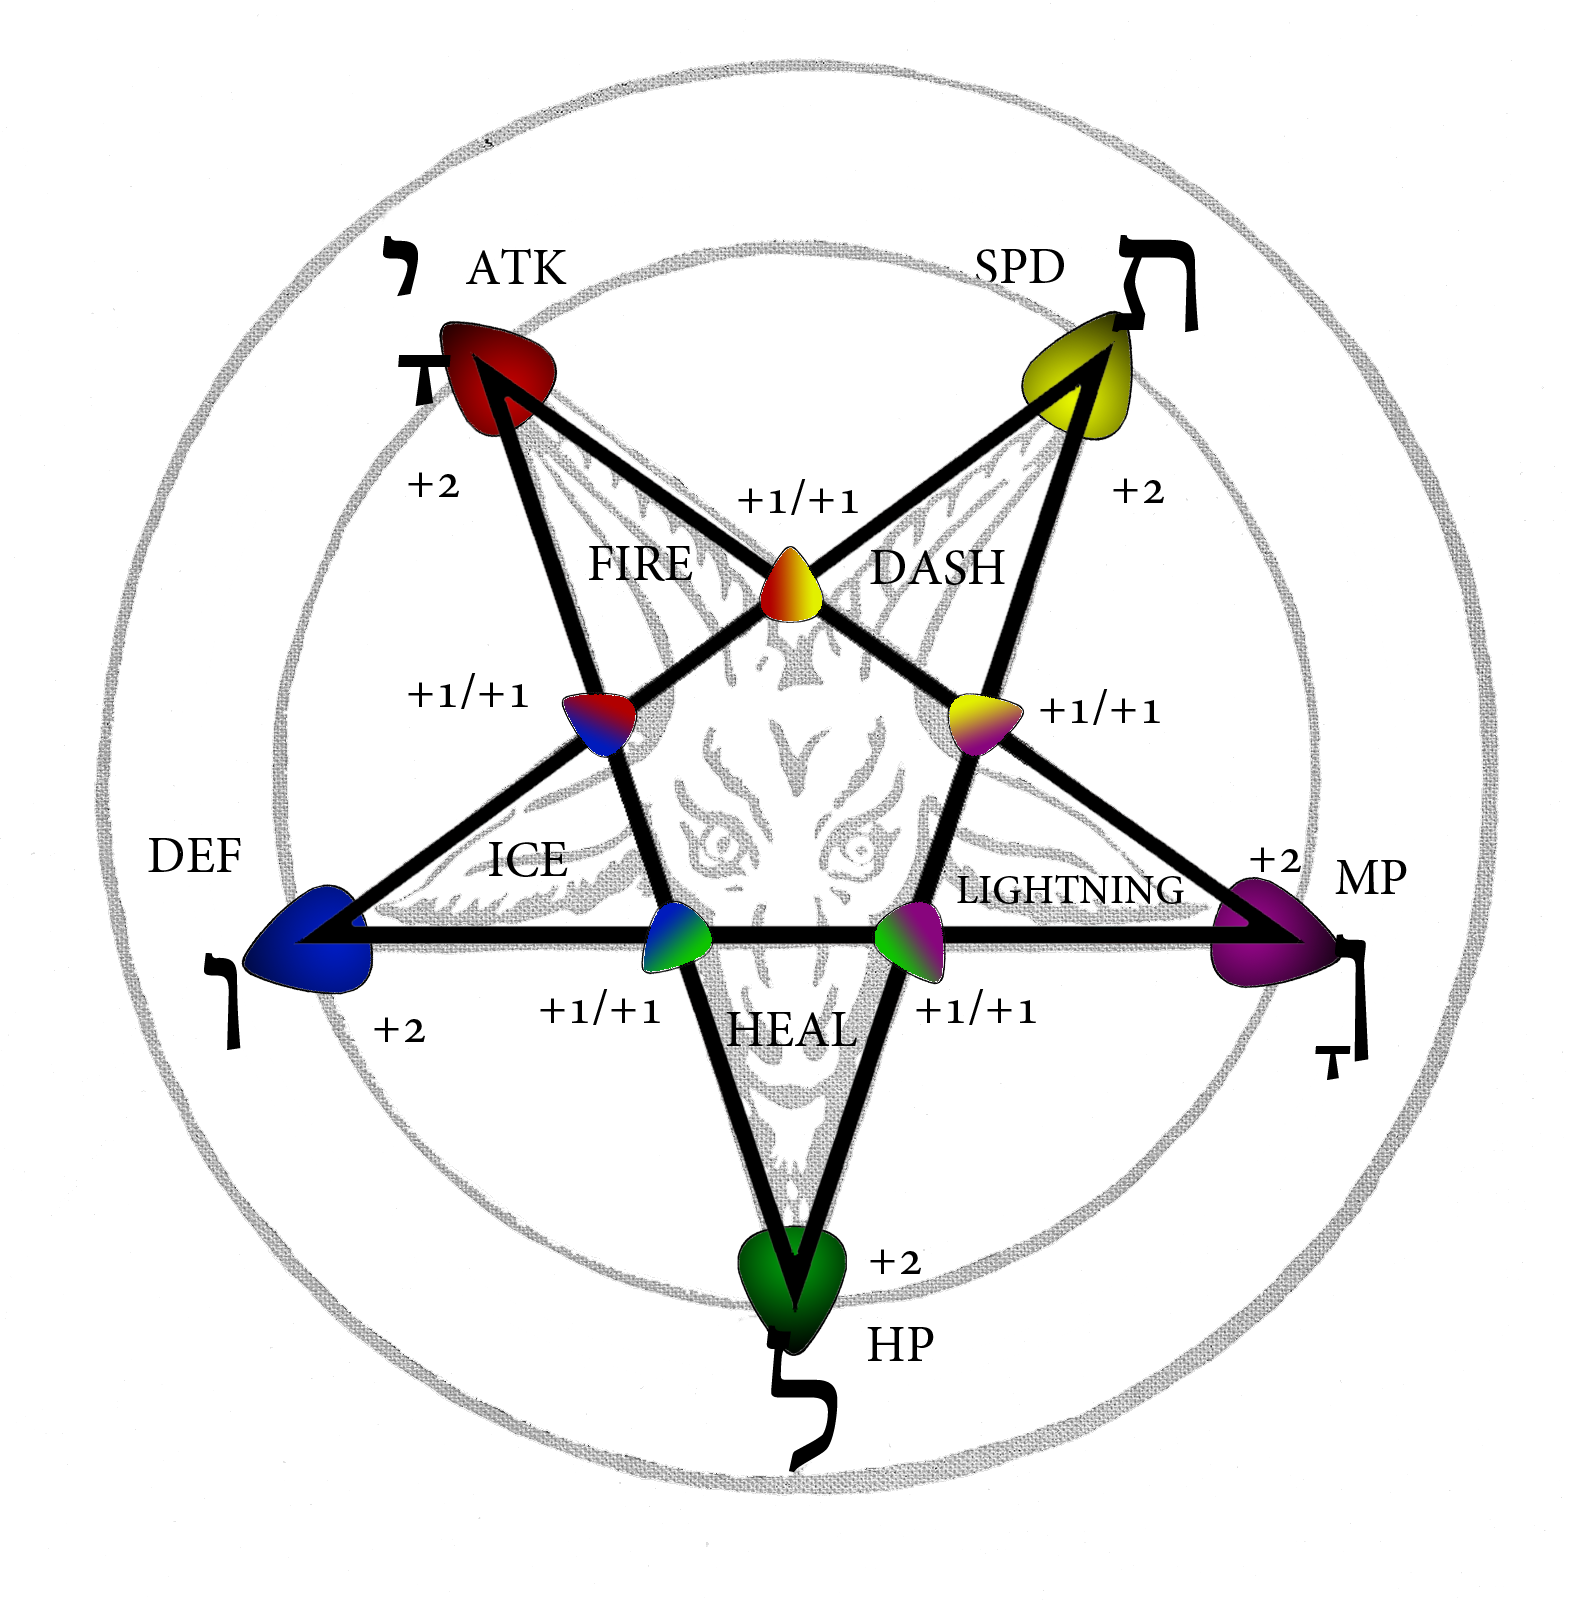
\includegraphics[width=5in]{Graphics/LevelupPentagram.png}
\caption{The level-up pentagram.}
\label{Pentagram}

\end{figure}

Activating each node provides an increase to one or more of the player's stats.  The nodes on the outer points provide +2 points to Attack, Defense, HP, MP, and Speed, while the inner nodes provide +1 points to 2 stats, determined by which outer points they are adjacent to.  For example, the inner node adjacent to both the +2 HP and +2 MP nodes provides +1 to both HP and MP.  Although increase of stats is abstracted into a simple, consistent point system, the effects of a single point are different for each stat, and are illustrated in figure \ref{LevelupStats}.

\begin{figure}[h!]
\begin{tabular}{|r|l|}
\hline
Stat & 1 Point Means \\
\hline
HP & One extra health tank (+100 HP). \\
MP & One extra magic tank (+100 MP). \\
Speed & +10 world units per second. \\
Defense & +10 defense. \\
Attack & +10 attack. \\
\hline
\end{tabular}
\caption{Level-Up Stat Increases}
\label{LevelupStats}
\end{figure}

Gaining abilities is also achieved using the pentagram.  Each of the triangular points of the pentagram is associated with an ability (Fire, Dash, Lightning, Heal, Ice).  Activating all nodes surrounding that ability gives that ability to the player.  The abilities are generally themed such that each one corresponds roughly to the stat associated with its triangle.  For example, activating all HP nodes gives the player the Heal ability, which restores HP.  Similarly, Activating all speed nodes gives the player the Dash ability, which allows fast movement.

Because the level-up system is intended to encourage replayability, a player will not be able to activate all nodes or gain all abilities in a single play-through.  Because there are a total of 10 nodes, the player will be limited to a maximum of 5 level-ups throughout the course of the game, ensuring that only a limited selection of abilities will be chosen by the player.  It is worth noting that the Pentagram was initially intended to be much more extensive, with each triangle segmented into 4 sub-triangles, giving a total of 25 nodes and 20 unique abilities.  However, due to limited time and resources, as well as the fact that only a demo version is being developed, the pentagram was reduced in size.

\subsection{Controls}

The primary intention when designing controls for this game is to keep them as simple as possible, while maintaining a degree of flexibility that allows for interesting and unique gameplay strategies.  Another goal is to ensure that we use a scheme that experienced gamers are used to, allowing them to pick up gameplay easily.  Figure \ref{ControlsTable} summarizes the controls.

Like first person shooters, the WASD keys are used as the primary movement keys.  The A key moves the player left, and the D key moves the player right.  Since the down direction has little purpose in a side-scroller, the S key is used for ducking.

Jumping is accomplished using the space key.  There will be a short delay after pressing the jump key.  Depending on how long the player holds the jump key, their upward velocity will be affected, easily allowing the player to control the height of their jumps.  It is also fully possible to control the in-air trajectory by moving left and right.  Although this is unrealistic, experience has taught us that this is the preferred way to control jumping in a side-scroller.  Wall-jumping is accomplished by jumping when next to a vertical wall.  This can be done indefinitely (similar to wall jumping in Mega Man X).  A high-jump can be accomlplished by crouching before jumping.

Despite being a sidescroller, the inclusion of the ability to aim inspired us to use the conventions of first-person shooters.  Aiming and attacking is done with the mouse.  The left mouse button executes the primary attack, which may be aimed in any direction.  Additionally, the orientation of the player's character (left or right).  is determined by the position of the mouse.  This enables the player to move forwards and backwards easily while aiming at any desired target.

Special abilities are used with the right mouse button.  There is at most one active special ability, which may either be selected by using the number keys or by using the mouse's scroll wheel.  This scheme should be familiar to most first-person shooter players, who are used to selecting weapons in this way.  The fire ability functions much like a normal attack, and can similarly be aimed in any direction.  The lightning ability is the only projectile ability, and can be aimed at any target on the screen.  Ice and heal cause effects local only to the player, and therefore aiming has no effect on them.

Dash is a special case of abilities.  Rather than being selected and used with the right mouse button, it is mapped to movement keys.  The Q and E keys allow left- and right-dashing respectively.  They were chosen due to their close proximity to A and D, the left and right movement keys.

\begin{figure}[h!]
\begin{tabular}{|r|l|}
\hline
Key & Action \\
\hline
A & Move left \\
D & Move right \\
S & Crouch \\
Q & Dash left \\
E & Dash right \\
Space & Jump \\
Mouse & Aim \\
Left Mouse & Attack \\
Right Mouse & Special ability \\
Mouse Wheel & Change special ability \\
1 & Select Lightning \\
2 & Select Fire \\
3 & Select Ice \\
4 & Select Heal \\
\hline
\end{tabular}
\caption{Summary of Controls}
\label{ControlsTable}
\end{figure}

\begin{figure}[h!]
\begin{tabular}{|r|l|}
\hline
Stat & 1 Point Means \\
\hline
HP & One extra health tank (+100 HP). \\
MP & One extra magic tank (+100 MP). \\
Speed & +10 world units per second. \\
Defense & +10 defense. \\
Attack & +10 attack. \\
\hline
\end{tabular}
\caption{Level-Up Stat Increases}
\label{LevelupStats}
\end{figure}

\subsection{Data Management and Flow}

As this is a roguelike game which includes permanent death, there is no permanent save option.  However, as challenging or frustrating as this may be to players, we do not wish to frustrate them further by interfering with their lives.  To this end, a quick-save feature will be implemented, which allows a player to suspend the game through use of a "save and quit" option.  When the game is restarted, the player has the option to continue from their saved game.  When the continue option is selected, the saved game is deleted.

The quicksave will save the state of the world in a simple text file.  The randomly-generated level structure can easily be output to and read from a string (see section \ref{RoomAndEnemy}
for details on string representation of levels).  In addition to this, only a few other key pieces of information are required: enemy data and player data.

Enemy data will record the current location, stats, and state of each enemy object in the game.  Position will be represented as a simple tuple of 3 floating-point numbers (i.e. (1,0,0)).  The stats object will also have a simple string representation, which can be translated at run-time into a stats object.  As C\# provides default conversion of enumerated types to strings, storing entity states will be as simple as writing the corresponding string value.

Player data is slightly more complex than enemy data.  While the simple matters of stats, state, and location are the same, the player also has experience and abilities.  The save file will include a special section dedicated to these aspects.  First of all, the current level and amount of experience gained is stored in the file.  Second, in order to track progress in the level-up pentagram, each node of the pentagram will be given a name (i.e. HP\_MP could represent HP/MP +1 / +1 node).  A list of these nodes will be stored in the section, allowing the corresponding nodes to be activated upon loading the game.

At this time, there are no plans to use encryption methods to protect the game's save data.

\section{User Interface}

\subsection{Game Shell}

Game gui is rather simple and straight forward.  This section includes the diagram of the main screens and a short description of each screen.

\subsection{Play Screen}

The play screen consists of two different parts. The first lower part is the game scene.  Only a single room is shown to the player at any given time. The player can go to other rooms by digging through the snow which connects two neighbouring rooms.  In each room there might be one or several enemies.  Each room consists of several blocks of ice and rocks and has architecture based on one of the pre-defined room types.

\paragraph{Player Status}
The top part of the game scene is used for presenting the player information.  The left corner displays HP and MP tanks (each worth 100 HP or MP units).  This number of HP tanks is limited, but may increase as a level up reward.  MP is also a limited resource for the player.  It is important to display this so that the player understands this limitation.

In the middle top part of the game screen, there will be two other sections.  The first one is the ability line which displays graphical representation of all possible abilities that the player can achieve thorough level-ups.  Locked and unlocked abilities have different colors; moreover only the active one is highlighted. Player can achieve all abilities visible in figure \ref{Pentagram}. The graphic representation for all of these will be in this section.

On the right-hand side of the top of the screen, a small local map is displayed.  This includes the current room and all rooms immediately adjacent to the it.

\begin{figure}[h!]
{\scalefont{0.6}
% Graphic for TeX using PGF
% Title: C:\Users\Kaylen\CotWM\Doc\Graphics\menu.dia
% Creator: Dia v0.97.1
% CreationDate: Mon Mar 12 11:25:24 2012
% For: Kaylen
% \usepackage{tikz}
% The following commands are not supported in PSTricks at present
% We define them conditionally, so when they are implemented,
% this pgf file will use them.
\ifx\du\undefined
  \newlength{\du}
\fi
\setlength{\du}{15\unitlength}
\begin{tikzpicture}
\pgftransformxscale{0.547029}
\pgftransformyscale{-0.547029}
\definecolor{dialinecolor}{rgb}{0.000000, 0.000000, 0.000000}
\pgfsetstrokecolor{dialinecolor}
\definecolor{dialinecolor}{rgb}{1.000000, 1.000000, 1.000000}
\pgfsetfillcolor{dialinecolor}
\pgfsetlinewidth{0.100000\du}
\pgfsetdash{}{0pt}
\pgfsetdash{}{0pt}
\pgfsetmiterjoin
\pgfsetbuttcap
{
\definecolor{dialinecolor}{rgb}{0.000000, 0.000000, 0.000000}
\pgfsetfillcolor{dialinecolor}
% was here!!!
\pgfsetarrowsend{stealth}
{\pgfsetcornersarced{\pgfpoint{0.000000\du}{0.000000\du}}\definecolor{dialinecolor}{rgb}{0.000000, 0.000000, 0.000000}
\pgfsetstrokecolor{dialinecolor}
\draw (20.087500\du,24.060000\du)--(20.087500\du,1.982510\du)--(13.425000\du,1.982510\du)--(13.425000\du,0.241166\du);
}}
\definecolor{dialinecolor}{rgb}{1.000000, 1.000000, 1.000000}
\pgfsetfillcolor{dialinecolor}
\fill (6.650000\du,-11.350000\du)--(6.650000\du,-6.750000\du)--(12.950000\du,-6.750000\du)--(12.950000\du,-11.350000\du)--cycle;
\pgfsetlinewidth{0.100000\du}
\pgfsetdash{}{0pt}
\pgfsetdash{}{0pt}
\pgfsetmiterjoin
\definecolor{dialinecolor}{rgb}{0.000000, 0.000000, 0.000000}
\pgfsetstrokecolor{dialinecolor}
\draw (6.650000\du,-11.350000\du)--(6.650000\du,-6.750000\du)--(12.950000\du,-6.750000\du)--(12.950000\du,-11.350000\du)--cycle;
% setfont left to latex
\definecolor{dialinecolor}{rgb}{0.000000, 0.000000, 0.000000}
\pgfsetstrokecolor{dialinecolor}
\node at (9.800000\du,-8.810000\du){title};
\definecolor{dialinecolor}{rgb}{1.000000, 1.000000, 1.000000}
\pgfsetfillcolor{dialinecolor}
\fill (7.790000\du,15.962500\du)--(7.790000\du,19.491166\du)--(13.650000\du,19.491166\du)--(13.650000\du,15.962500\du)--cycle;
\pgfsetlinewidth{0.100000\du}
\pgfsetdash{}{0pt}
\pgfsetdash{}{0pt}
\pgfsetmiterjoin
\definecolor{dialinecolor}{rgb}{0.000000, 0.000000, 0.000000}
\pgfsetstrokecolor{dialinecolor}
\draw (7.790000\du,15.962500\du)--(7.790000\du,19.491166\du)--(13.650000\du,19.491166\du)--(13.650000\du,15.962500\du)--cycle;
% setfont left to latex
\definecolor{dialinecolor}{rgb}{0.000000, 0.000000, 0.000000}
\pgfsetstrokecolor{dialinecolor}
\node at (10.720000\du,17.566833\du){key intruduction };
% setfont left to latex
\definecolor{dialinecolor}{rgb}{0.000000, 0.000000, 0.000000}
\pgfsetstrokecolor{dialinecolor}
\node at (10.720000\du,18.366833\du){page};
\definecolor{dialinecolor}{rgb}{1.000000, 1.000000, 1.000000}
\pgfsetfillcolor{dialinecolor}
\fill (7.650000\du,22.075000\du)--(7.650000\du,24.862500\du)--(14.075000\du,24.862500\du)--(14.075000\du,22.075000\du)--cycle;
\pgfsetlinewidth{0.100000\du}
\pgfsetdash{}{0pt}
\pgfsetdash{}{0pt}
\pgfsetmiterjoin
\definecolor{dialinecolor}{rgb}{0.000000, 0.000000, 0.000000}
\pgfsetstrokecolor{dialinecolor}
\draw (7.650000\du,22.075000\du)--(7.650000\du,24.862500\du)--(14.075000\du,24.862500\du)--(14.075000\du,22.075000\du)--cycle;
% setfont left to latex
\definecolor{dialinecolor}{rgb}{0.000000, 0.000000, 0.000000}
\pgfsetstrokecolor{dialinecolor}
\node at (10.862500\du,23.708750\du){game scene};
\definecolor{dialinecolor}{rgb}{1.000000, 1.000000, 1.000000}
\pgfsetfillcolor{dialinecolor}
\fill (7.750000\du,29.670000\du)--(7.750000\du,31.925000\du)--(13.755000\du,31.925000\du)--(13.755000\du,29.670000\du)--cycle;
\pgfsetlinewidth{0.100000\du}
\pgfsetdash{}{0pt}
\pgfsetdash{}{0pt}
\pgfsetmiterjoin
\definecolor{dialinecolor}{rgb}{0.000000, 0.000000, 0.000000}
\pgfsetstrokecolor{dialinecolor}
\draw (7.750000\du,29.670000\du)--(7.750000\du,31.925000\du)--(13.755000\du,31.925000\du)--(13.755000\du,29.670000\du)--cycle;
% setfont left to latex
\definecolor{dialinecolor}{rgb}{0.000000, 0.000000, 0.000000}
\pgfsetstrokecolor{dialinecolor}
\node at (10.752500\du,31.037500\du){ending};
\definecolor{dialinecolor}{rgb}{1.000000, 1.000000, 1.000000}
\pgfsetfillcolor{dialinecolor}
\fill (16.295200\du,18.148400\du)--(16.295200\du,20.562500\du)--(21.420200\du,20.562500\du)--(21.420200\du,18.148400\du)--cycle;
\pgfsetlinewidth{0.100000\du}
\pgfsetdash{}{0pt}
\pgfsetdash{}{0pt}
\pgfsetmiterjoin
\definecolor{dialinecolor}{rgb}{0.000000, 0.000000, 0.000000}
\pgfsetstrokecolor{dialinecolor}
\draw (16.295200\du,18.148400\du)--(16.295200\du,20.562500\du)--(21.420200\du,20.562500\du)--(21.420200\du,18.148400\du)--cycle;
% setfont left to latex
\definecolor{dialinecolor}{rgb}{0.000000, 0.000000, 0.000000}
\pgfsetstrokecolor{dialinecolor}
\node at (18.857700\du,19.595450\du){status screen};
\definecolor{dialinecolor}{rgb}{1.000000, 1.000000, 1.000000}
\pgfsetfillcolor{dialinecolor}
\fill (18.450000\du,24.060000\du)--(18.450000\du,26.562500\du)--(25.000000\du,26.562500\du)--(25.000000\du,24.060000\du)--cycle;
\pgfsetlinewidth{0.100000\du}
\pgfsetdash{}{0pt}
\pgfsetdash{}{0pt}
\pgfsetmiterjoin
\definecolor{dialinecolor}{rgb}{0.000000, 0.000000, 0.000000}
\pgfsetstrokecolor{dialinecolor}
\draw (18.450000\du,24.060000\du)--(18.450000\du,26.562500\du)--(25.000000\du,26.562500\du)--(25.000000\du,24.060000\du)--cycle;
% setfont left to latex
\definecolor{dialinecolor}{rgb}{0.000000, 0.000000, 0.000000}
\pgfsetstrokecolor{dialinecolor}
\node at (21.725000\du,25.551250\du){pause menu};
% setfont left to latex
\definecolor{dialinecolor}{rgb}{0.000000, 0.000000, 0.000000}
\pgfsetstrokecolor{dialinecolor}
\node[anchor=west] at (9.800000\du,-9.050000\du){};
\definecolor{dialinecolor}{rgb}{1.000000, 1.000000, 1.000000}
\pgfsetfillcolor{dialinecolor}
\fill (6.255000\du,-4.005000\du)--(6.255000\du,0.241166\du)--(13.425000\du,0.241166\du)--(13.425000\du,-4.005000\du)--cycle;
\pgfsetlinewidth{0.100000\du}
\pgfsetdash{}{0pt}
\pgfsetdash{}{0pt}
\pgfsetmiterjoin
\definecolor{dialinecolor}{rgb}{0.000000, 0.000000, 0.000000}
\pgfsetstrokecolor{dialinecolor}
\draw (6.255000\du,-4.005000\du)--(6.255000\du,0.241166\du)--(13.425000\du,0.241166\du)--(13.425000\du,-4.005000\du)--cycle;
% setfont left to latex
\definecolor{dialinecolor}{rgb}{0.000000, 0.000000, 0.000000}
\pgfsetstrokecolor{dialinecolor}
\node at (9.840000\du,-1.641917\du){main menu};
\pgfsetlinewidth{0.100000\du}
\pgfsetbuttcap
\pgfsetdash{}{0pt}
{
\definecolor{dialinecolor}{rgb}{0.000000, 0.000000, 0.000000}
\pgfsetfillcolor{dialinecolor}
% was here!!!
\pgfsetarrowsstart{latex}
\definecolor{dialinecolor}{rgb}{0.000000, 0.000000, 0.000000}
\pgfsetstrokecolor{dialinecolor}
\draw (18.705000\du,-1.882500\du)--(13.425000\du,-1.881920\du);
}
% setfont left to latex
\pgfsetlinewidth{0.100000\du}
\pgfsetbuttcap
\pgfsetdash{}{0pt}
{
\definecolor{dialinecolor}{rgb}{0.000000, 0.000000, 0.000000}
\pgfsetfillcolor{dialinecolor}
% was here!!!
\pgfsetarrowsstart{latex}
\definecolor{dialinecolor}{rgb}{0.000000, 0.000000, 0.000000}
\pgfsetstrokecolor{dialinecolor}
\draw (9.840000\du,-4.005000\du)--(9.818613\du,-6.702400\du);
}
% setfont left to latex
\pgfsetlinewidth{0.100000\du}
\pgfsetbuttcap
\pgfsetdash{}{0pt}
{
\definecolor{dialinecolor}{rgb}{0.000000, 0.000000, 0.000000}
\pgfsetfillcolor{dialinecolor}
% was here!!!
\pgfsetarrowsstart{latex}
\definecolor{dialinecolor}{rgb}{0.000000, 0.000000, 0.000000}
\pgfsetstrokecolor{dialinecolor}
\draw (10.862500\du,22.075000\du)--(10.720000\du,19.491200\du);
}
% setfont left to latex
% setfont left to latex
\definecolor{dialinecolor}{rgb}{0.000000, 0.000000, 0.000000}
\pgfsetstrokecolor{dialinecolor}
\node[anchor=west] at (33.362500\du,19.408800\du){};
% setfont left to latex
\definecolor{dialinecolor}{rgb}{0.000000, 0.000000, 0.000000}
\pgfsetstrokecolor{dialinecolor}
\node[anchor=west] at (33.362500\du,19.408800\du){};
% setfont left to latex
\definecolor{dialinecolor}{rgb}{0.000000, 0.000000, 0.000000}
\pgfsetstrokecolor{dialinecolor}
\node[anchor=west] at (21.725000\du,25.311300\du){};
\definecolor{dialinecolor}{rgb}{1.000000, 1.000000, 1.000000}
\pgfsetfillcolor{dialinecolor}
\fill (7.000000\du,11.262500\du)--(7.000000\du,13.695000\du)--(13.245000\du,13.695000\du)--(13.245000\du,11.262500\du)--cycle;
\pgfsetlinewidth{0.100000\du}
\pgfsetdash{}{0pt}
\pgfsetdash{}{0pt}
\pgfsetmiterjoin
\definecolor{dialinecolor}{rgb}{0.000000, 0.000000, 0.000000}
\pgfsetstrokecolor{dialinecolor}
\draw (7.000000\du,11.262500\du)--(7.000000\du,13.695000\du)--(13.245000\du,13.695000\du)--(13.245000\du,11.262500\du)--cycle;
% setfont left to latex
\definecolor{dialinecolor}{rgb}{0.000000, 0.000000, 0.000000}
\pgfsetstrokecolor{dialinecolor}
\node at (10.122500\du,12.718750\du){introduction};
\pgfsetlinewidth{0.100000\du}
\pgfsetdash{}{0pt}
\pgfsetdash{}{0pt}
\pgfsetbuttcap
{
\definecolor{dialinecolor}{rgb}{0.000000, 0.000000, 0.000000}
\pgfsetfillcolor{dialinecolor}
% was here!!!
\pgfsetarrowsend{stealth}
\definecolor{dialinecolor}{rgb}{0.000000, 0.000000, 0.000000}
\pgfsetstrokecolor{dialinecolor}
\draw (23.288300\du,-1.511500\du)--(23.288300\du,-1.511500\du);
}
\pgfsetlinewidth{0.100000\du}
\pgfsetbuttcap
\pgfsetdash{}{0pt}
{
\definecolor{dialinecolor}{rgb}{0.000000, 0.000000, 0.000000}
\pgfsetfillcolor{dialinecolor}
% was here!!!
\pgfsetarrowsstart{latex}
\definecolor{dialinecolor}{rgb}{0.000000, 0.000000, 0.000000}
\pgfsetstrokecolor{dialinecolor}
\draw (10.155000\du,15.712500\du)--(10.122500\du,13.695000\du);
}
% setfont left to latex
% setfont left to latex
\definecolor{dialinecolor}{rgb}{0.000000, 0.000000, 0.000000}
\pgfsetstrokecolor{dialinecolor}
\node[anchor=west] at (10.720000\du,17.726800\du){};
\pgfsetlinewidth{0.100000\du}
\pgfsetdash{}{0pt}
\pgfsetdash{}{0pt}
\pgfsetmiterjoin
\pgfsetbuttcap
{
\definecolor{dialinecolor}{rgb}{0.000000, 0.000000, 0.000000}
\pgfsetfillcolor{dialinecolor}
% was here!!!
\pgfsetarrowsend{stealth}
{\pgfsetcornersarced{\pgfpoint{0.000000\du}{0.000000\du}}\definecolor{dialinecolor}{rgb}{0.000000, 0.000000, 0.000000}
\pgfsetstrokecolor{dialinecolor}
\draw (6.441150\du,6.257950\du)--(6.441150\du,6.462500\du)--(0.040000\du,6.462500\du)--(0.040000\du,10.862500\du);
}}
\definecolor{dialinecolor}{rgb}{1.000000, 1.000000, 1.000000}
\pgfsetfillcolor{dialinecolor}
\fill (-0.195000\du,11.062500\du)--(-0.195000\du,14.062500\du)--(4.745000\du,14.062500\du)--(4.745000\du,11.062500\du)--cycle;
\pgfsetlinewidth{0.100000\du}
\pgfsetdash{}{0pt}
\pgfsetdash{}{0pt}
\pgfsetmiterjoin
\definecolor{dialinecolor}{rgb}{0.000000, 0.000000, 0.000000}
\pgfsetstrokecolor{dialinecolor}
\draw (-0.195000\du,11.062500\du)--(-0.195000\du,14.062500\du)--(4.745000\du,14.062500\du)--(4.745000\du,11.062500\du)--cycle;
% setfont left to latex
\definecolor{dialinecolor}{rgb}{0.000000, 0.000000, 0.000000}
\pgfsetstrokecolor{dialinecolor}
\node at (2.275000\du,12.802500\du){warning page};
\pgfsetlinewidth{0.100000\du}
\pgfsetdash{}{0pt}
\pgfsetdash{}{0pt}
\pgfsetbuttcap
{
\definecolor{dialinecolor}{rgb}{0.000000, 0.000000, 0.000000}
\pgfsetfillcolor{dialinecolor}
% was here!!!
\pgfsetarrowsend{stealth}
\definecolor{dialinecolor}{rgb}{0.000000, 0.000000, 0.000000}
\pgfsetstrokecolor{dialinecolor}
\draw (4.745000\du,12.562500\du)--(7.000000\du,12.478800\du);
}
\pgfsetlinewidth{0.100000\du}
\pgfsetdash{}{0pt}
\pgfsetdash{}{0pt}
\pgfsetmiterjoin
\pgfsetbuttcap
{
\definecolor{dialinecolor}{rgb}{0.000000, 0.000000, 0.000000}
\pgfsetfillcolor{dialinecolor}
% was here!!!
\pgfsetarrowsend{stealth}
{\pgfsetcornersarced{\pgfpoint{0.000000\du}{0.000000\du}}\definecolor{dialinecolor}{rgb}{0.000000, 0.000000, 0.000000}
\pgfsetstrokecolor{dialinecolor}
\draw (1.040000\du,14.062500\du)--(1.040000\du,23.468750\du)--(7.650000\du,23.468750\du);
}}
% setfont left to latex
\definecolor{dialinecolor}{rgb}{0.000000, 0.000000, 0.000000}
\pgfsetstrokecolor{dialinecolor}
\node[anchor=west] at (2.275000\du,12.562500\du){};
% setfont left to latex
\definecolor{dialinecolor}{rgb}{0.000000, 0.000000, 0.000000}
\pgfsetstrokecolor{dialinecolor}
\node[anchor=west] at (8.034930\du,8.333330\du){};
% setfont left to latex
\definecolor{dialinecolor}{rgb}{0.000000, 0.000000, 0.000000}
\pgfsetstrokecolor{dialinecolor}
\node[anchor=west] at (8.034930\du,8.333330\du){};
\definecolor{dialinecolor}{rgb}{1.000000, 1.000000, 1.000000}
\pgfsetfillcolor{dialinecolor}
\fill (10.074291\du,2.840690\du)--(13.707433\du,6.257946\du)--(10.074291\du,9.675202\du)--(6.441150\du,6.257946\du)--cycle;
\pgfsetlinewidth{0.100000\du}
\pgfsetdash{}{0pt}
\pgfsetdash{}{0pt}
\pgfsetmiterjoin
\definecolor{dialinecolor}{rgb}{0.000000, 0.000000, 0.000000}
\pgfsetstrokecolor{dialinecolor}
\draw (10.074291\du,2.840690\du)--(13.707433\du,6.257946\du)--(10.074291\du,9.675202\du)--(6.441150\du,6.257946\du)--cycle;
% setfont left to latex
\definecolor{dialinecolor}{rgb}{0.000000, 0.000000, 0.000000}
\pgfsetstrokecolor{dialinecolor}
\node at (10.074291\du,6.097946\du){have a};
% setfont left to latex
\definecolor{dialinecolor}{rgb}{0.000000, 0.000000, 0.000000}
\pgfsetstrokecolor{dialinecolor}
\node at (10.074291\du,6.897946\du){ saved game?};
\pgfsetlinewidth{0.100000\du}
\pgfsetdash{}{0pt}
\pgfsetdash{}{0pt}
\pgfsetbuttcap
{
\definecolor{dialinecolor}{rgb}{0.000000, 0.000000, 0.000000}
\pgfsetfillcolor{dialinecolor}
% was here!!!
\pgfsetarrowsend{stealth}
\definecolor{dialinecolor}{rgb}{0.000000, 0.000000, 0.000000}
\pgfsetstrokecolor{dialinecolor}
\draw (10.105000\du,0.332510\du)--(10.074300\du,2.840690\du);
}
\pgfsetlinewidth{0.100000\du}
\pgfsetdash{}{0pt}
\pgfsetdash{}{0pt}
\pgfsetbuttcap
{
\definecolor{dialinecolor}{rgb}{0.000000, 0.000000, 0.000000}
\pgfsetfillcolor{dialinecolor}
% was here!!!
\pgfsetarrowsend{stealth}
\definecolor{dialinecolor}{rgb}{0.000000, 0.000000, 0.000000}
\pgfsetstrokecolor{dialinecolor}
\draw (10.074300\du,9.675200\du)--(10.122500\du,11.262500\du);
}
\definecolor{dialinecolor}{rgb}{1.000000, 1.000000, 1.000000}
\pgfsetfillcolor{dialinecolor}
\fill (18.705000\du,-2.462500\du)--(18.705000\du,-0.142500\du)--(25.005000\du,-0.142500\du)--(25.005000\du,-2.462500\du)--cycle;
\pgfsetlinewidth{0.100000\du}
\pgfsetdash{}{0pt}
\pgfsetdash{}{0pt}
\pgfsetmiterjoin
\definecolor{dialinecolor}{rgb}{0.000000, 0.000000, 0.000000}
\pgfsetstrokecolor{dialinecolor}
\draw (18.705000\du,-2.462500\du)--(18.705000\du,-0.142500\du)--(25.005000\du,-0.142500\du)--(25.005000\du,-2.462500\du)--cycle;
% setfont left to latex
\definecolor{dialinecolor}{rgb}{0.000000, 0.000000, 0.000000}
\pgfsetstrokecolor{dialinecolor}
\node at (21.855000\du,-1.062500\du){options};
\pgfsetlinewidth{0.100000\du}
\pgfsetdash{}{0pt}
\pgfsetdash{}{0pt}
\pgfsetmiterjoin
\pgfsetbuttcap
{
\definecolor{dialinecolor}{rgb}{0.000000, 0.000000, 0.000000}
\pgfsetfillcolor{dialinecolor}
% was here!!!
\pgfsetarrowsend{stealth}
{\pgfsetcornersarced{\pgfpoint{0.000000\du}{0.000000\du}}\definecolor{dialinecolor}{rgb}{0.000000, 0.000000, 0.000000}
\pgfsetstrokecolor{dialinecolor}
\draw (14.075000\du,22.771875\du)--(15.185100\du,22.771875\du)--(15.185100\du,19.355450\du)--(16.295200\du,19.355450\du);
}}
\pgfsetlinewidth{0.100000\du}
\pgfsetdash{}{0pt}
\pgfsetdash{}{0pt}
\pgfsetmiterjoin
\pgfsetbuttcap
{
\definecolor{dialinecolor}{rgb}{0.000000, 0.000000, 0.000000}
\pgfsetfillcolor{dialinecolor}
% was here!!!
\pgfsetarrowsend{stealth}
{\pgfsetcornersarced{\pgfpoint{0.000000\du}{0.000000\du}}\definecolor{dialinecolor}{rgb}{0.000000, 0.000000, 0.000000}
\pgfsetstrokecolor{dialinecolor}
\draw (12.468750\du,24.862500\du)--(12.496947\du,24.862500\du)--(12.496947\du,25.936900\du)--(18.450000\du,25.936900\du);
}}
\definecolor{dialinecolor}{rgb}{1.000000, 1.000000, 1.000000}
\pgfsetfillcolor{dialinecolor}
\fill (21.824630\du,29.119700\du)--(24.204960\du,30.822365\du)--(21.824630\du,32.525030\du)--(19.444300\du,30.822365\du)--cycle;
\pgfsetlinewidth{0.100000\du}
\pgfsetdash{}{0pt}
\pgfsetdash{}{0pt}
\pgfsetmiterjoin
\definecolor{dialinecolor}{rgb}{0.000000, 0.000000, 0.000000}
\pgfsetstrokecolor{dialinecolor}
\draw (21.824630\du,29.119700\du)--(24.204960\du,30.822365\du)--(21.824630\du,32.525030\du)--(19.444300\du,30.822365\du)--cycle;
% setfont left to latex
\definecolor{dialinecolor}{rgb}{0.000000, 0.000000, 0.000000}
\pgfsetstrokecolor{dialinecolor}
\node at (21.824630\du,31.062365\du){exit?};
\pgfsetlinewidth{0.100000\du}
\pgfsetdash{}{0pt}
\pgfsetdash{}{0pt}
\pgfsetmiterjoin
\pgfsetbuttcap
{
\definecolor{dialinecolor}{rgb}{0.000000, 0.000000, 0.000000}
\pgfsetfillcolor{dialinecolor}
% was here!!!
\pgfsetarrowsend{stealth}
{\pgfsetcornersarced{\pgfpoint{0.000000\du}{0.000000\du}}\definecolor{dialinecolor}{rgb}{0.000000, 0.000000, 0.000000}
\pgfsetstrokecolor{dialinecolor}
\draw (24.205000\du,30.822300\du)--(24.205000\du,30.725000\du)--(25.000000\du,30.725000\du)--(25.000000\du,26.562500\du);
}}
\pgfsetlinewidth{0.100000\du}
\pgfsetdash{}{0pt}
\pgfsetdash{}{0pt}
\pgfsetbuttcap
{
\definecolor{dialinecolor}{rgb}{0.000000, 0.000000, 0.000000}
\pgfsetfillcolor{dialinecolor}
% was here!!!
\pgfsetarrowsend{stealth}
\definecolor{dialinecolor}{rgb}{0.000000, 0.000000, 0.000000}
\pgfsetstrokecolor{dialinecolor}
\draw (21.725000\du,26.562500\du)--(21.824700\du,29.119700\du);
}
\pgfsetlinewidth{0.100000\du}
\pgfsetdash{}{0pt}
\pgfsetdash{}{0pt}
\pgfsetmiterjoin
\pgfsetbuttcap
{
\definecolor{dialinecolor}{rgb}{0.000000, 0.000000, 0.000000}
\pgfsetfillcolor{dialinecolor}
% was here!!!
\pgfsetarrowsend{stealth}
{\pgfsetcornersarced{\pgfpoint{0.000000\du}{0.000000\du}}\definecolor{dialinecolor}{rgb}{0.000000, 0.000000, 0.000000}
\pgfsetstrokecolor{dialinecolor}
\draw (19.444300\du,30.822300\du)--(16.574700\du,30.822300\du)--(16.574700\du,30.797500\du)--(13.755000\du,30.797500\du);
}}
\pgfsetlinewidth{0.100000\du}
\pgfsetdash{}{0pt}
\pgfsetdash{}{0pt}
\pgfsetmiterjoin
\pgfsetbuttcap
{
\definecolor{dialinecolor}{rgb}{0.000000, 0.000000, 0.000000}
\pgfsetfillcolor{dialinecolor}
% was here!!!
\pgfsetarrowsend{stealth}
{\pgfsetcornersarced{\pgfpoint{0.000000\du}{0.000000\du}}\definecolor{dialinecolor}{rgb}{0.000000, 0.000000, 0.000000}
\pgfsetstrokecolor{dialinecolor}
\draw (6.255000\du,-1.881917\du)--(5.255000\du,-1.881917\du)--(5.255000\du,30.797500\du)--(7.750000\du,30.797500\du);
}}
\definecolor{dialinecolor}{rgb}{1.000000, 1.000000, 1.000000}
\pgfsetfillcolor{dialinecolor}
\fill (24.705000\du,18.157500\du)--(24.705000\du,20.407500\du)--(30.505000\du,20.407500\du)--(30.505000\du,18.157500\du)--cycle;
\pgfsetlinewidth{0.100000\du}
\pgfsetdash{}{0pt}
\pgfsetdash{}{0pt}
\pgfsetmiterjoin
\definecolor{dialinecolor}{rgb}{0.000000, 0.000000, 0.000000}
\pgfsetstrokecolor{dialinecolor}
\draw (24.705000\du,18.157500\du)--(24.705000\du,20.407500\du)--(30.505000\du,20.407500\du)--(30.505000\du,18.157500\du)--cycle;
% setfont left to latex
\definecolor{dialinecolor}{rgb}{0.000000, 0.000000, 0.000000}
\pgfsetstrokecolor{dialinecolor}
\node at (27.605000\du,19.522500\du){confirmation};
\pgfsetlinewidth{0.100000\du}
\pgfsetdash{}{0pt}
\pgfsetdash{}{0pt}
\pgfsetbuttcap
{
\definecolor{dialinecolor}{rgb}{0.000000, 0.000000, 0.000000}
\pgfsetfillcolor{dialinecolor}
% was here!!!
\pgfsetarrowsend{stealth}
\definecolor{dialinecolor}{rgb}{0.000000, 0.000000, 0.000000}
\pgfsetstrokecolor{dialinecolor}
\draw (21.420300\du,19.355500\du)--(24.505000\du,19.357500\du);
}
\pgfsetlinewidth{0.100000\du}
\pgfsetdash{}{0pt}
\pgfsetdash{}{0pt}
\pgfsetmiterjoin
\pgfsetbuttcap
{
\definecolor{dialinecolor}{rgb}{0.000000, 0.000000, 0.000000}
\pgfsetfillcolor{dialinecolor}
% was here!!!
\pgfsetarrowsend{stealth}
{\pgfsetcornersarced{\pgfpoint{0.000000\du}{0.000000\du}}\definecolor{dialinecolor}{rgb}{0.000000, 0.000000, 0.000000}
\pgfsetstrokecolor{dialinecolor}
\draw (29.055000\du,20.407500\du)--(29.055000\du,21.216074\du)--(10.862500\du,21.216074\du)--(10.862500\du,22.024648\du);
}}
% setfont left to latex
\definecolor{dialinecolor}{rgb}{0.000000, 0.000000, 0.000000}
\pgfsetstrokecolor{dialinecolor}
\node[anchor=west] at (21.725000\du,25.311300\du){};
\pgfsetlinewidth{0.100000\du}
\pgfsetdash{}{0pt}
\pgfsetdash{}{0pt}
\pgfsetbuttcap
{
\definecolor{dialinecolor}{rgb}{0.000000, 0.000000, 0.000000}
\pgfsetfillcolor{dialinecolor}
% was here!!!
\pgfsetarrowsend{stealth}
\definecolor{dialinecolor}{rgb}{0.000000, 0.000000, 0.000000}
\pgfsetstrokecolor{dialinecolor}
\draw (25.178100\du,24.470600\du)--(30.105000\du,24.520000\du);
}
\pgfsetlinewidth{0.100000\du}
\pgfsetdash{}{0pt}
\pgfsetdash{}{0pt}
\pgfsetmiterjoin
\pgfsetbuttcap
{
\definecolor{dialinecolor}{rgb}{0.000000, 0.000000, 0.000000}
\pgfsetfillcolor{dialinecolor}
% was here!!!
\pgfsetarrowsend{stealth}
{\pgfsetcornersarced{\pgfpoint{0.000000\du}{0.000000\du}}\definecolor{dialinecolor}{rgb}{0.000000, 0.000000, 0.000000}
\pgfsetstrokecolor{dialinecolor}
\draw (33.128100\du,26.870600\du)--(33.128100\du,28.270300\du)--(12.253750\du,28.270300\du)--(12.253750\du,29.670000\du);
}}
\definecolor{dialinecolor}{rgb}{1.000000, 1.000000, 1.000000}
\pgfsetfillcolor{dialinecolor}
\fill (33.158729\du,22.918000\du)--(36.728159\du,24.794300\du)--(33.158729\du,26.670601\du)--(29.589300\du,24.794300\du)--cycle;
\pgfsetlinewidth{0.100000\du}
\pgfsetdash{}{0pt}
\pgfsetdash{}{0pt}
\pgfsetmiterjoin
\definecolor{dialinecolor}{rgb}{0.000000, 0.000000, 0.000000}
\pgfsetstrokecolor{dialinecolor}
\draw (33.158729\du,22.918000\du)--(36.728159\du,24.794300\du)--(33.158729\du,26.670601\du)--(29.589300\du,24.794300\du)--cycle;
% setfont left to latex
\definecolor{dialinecolor}{rgb}{0.000000, 0.000000, 0.000000}
\pgfsetstrokecolor{dialinecolor}
\node at (33.158729\du,25.034300\du){quick save};
\definecolor{dialinecolor}{rgb}{1.000000, 1.000000, 1.000000}
\pgfsetfillcolor{dialinecolor}
\fill (38.005000\du,22.507500\du)--(38.005000\du,26.157500\du)--(44.555000\du,26.157500\du)--(44.555000\du,22.507500\du)--cycle;
\pgfsetlinewidth{0.100000\du}
\pgfsetdash{}{0pt}
\pgfsetdash{}{0pt}
\pgfsetmiterjoin
\definecolor{dialinecolor}{rgb}{0.000000, 0.000000, 0.000000}
\pgfsetstrokecolor{dialinecolor}
\draw (38.005000\du,22.507500\du)--(38.005000\du,26.157500\du)--(44.555000\du,26.157500\du)--(44.555000\du,22.507500\du)--cycle;
% setfont left to latex
\definecolor{dialinecolor}{rgb}{0.000000, 0.000000, 0.000000}
\pgfsetstrokecolor{dialinecolor}
\node at (41.280000\du,24.572500\du){game over };
\pgfsetlinewidth{0.100000\du}
\pgfsetdash{}{0pt}
\pgfsetdash{}{0pt}
\pgfsetmiterjoin
\pgfsetbuttcap
{
\definecolor{dialinecolor}{rgb}{0.000000, 0.000000, 0.000000}
\pgfsetfillcolor{dialinecolor}
% was here!!!
\pgfsetarrowsend{stealth}
{\pgfsetcornersarced{\pgfpoint{0.000000\du}{0.000000\du}}\definecolor{dialinecolor}{rgb}{0.000000, 0.000000, 0.000000}
\pgfsetstrokecolor{dialinecolor}
\draw (14.075000\du,23.468750\du)--(26.040000\du,23.468750\du)--(26.040000\du,22.507500\du)--(38.005000\du,22.507500\du);
}}
\pgfsetlinewidth{0.100000\du}
\pgfsetdash{}{0pt}
\pgfsetdash{}{0pt}
\pgfsetmiterjoin
\pgfsetbuttcap
{
\definecolor{dialinecolor}{rgb}{0.000000, 0.000000, 0.000000}
\pgfsetfillcolor{dialinecolor}
% was here!!!
\pgfsetarrowsend{stealth}
{\pgfsetcornersarced{\pgfpoint{0.000000\du}{0.000000\du}}\definecolor{dialinecolor}{rgb}{0.000000, 0.000000, 0.000000}
\pgfsetstrokecolor{dialinecolor}
\draw (38.005000\du,26.157500\du)--(38.005000\du,27.913750\du)--(7.750000\du,27.913750\du)--(7.750000\du,29.670000\du);
}}
\pgfsetlinewidth{0.100000\du}
\pgfsetdash{}{0pt}
\pgfsetdash{}{0pt}
\pgfsetmiterjoin
\pgfsetbuttcap
{
\definecolor{dialinecolor}{rgb}{0.000000, 0.000000, 0.000000}
\pgfsetfillcolor{dialinecolor}
% was here!!!
\pgfsetarrowsend{stealth}
{\pgfsetcornersarced{\pgfpoint{0.000000\du}{0.000000\du}}\definecolor{dialinecolor}{rgb}{0.000000, 0.000000, 0.000000}
\pgfsetstrokecolor{dialinecolor}
\draw (38.005000\du,22.507500\du)--(38.005000\du,3.150000\du)--(11.632500\du,3.150000\du)--(11.632500\du,0.241166\du);
}}
% setfont left to latex
\definecolor{dialinecolor}{rgb}{0.000000, 0.000000, 0.000000}
\pgfsetstrokecolor{dialinecolor}
\node[anchor=west] at (14.278200\du,20.120600\du){};
% setfont left to latex
\definecolor{dialinecolor}{rgb}{0.000000, 0.000000, 0.000000}
\pgfsetstrokecolor{dialinecolor}
\node[anchor=west] at (14.878200\du,22.470600\du){TAB};
% setfont left to latex
\definecolor{dialinecolor}{rgb}{0.000000, 0.000000, 0.000000}
\pgfsetstrokecolor{dialinecolor}
\node[anchor=west] at (22.228200\du,22.920600\du){GAME OVER};
% setfont left to latex
\definecolor{dialinecolor}{rgb}{0.000000, 0.000000, 0.000000}
\pgfsetstrokecolor{dialinecolor}
\node[anchor=west] at (15.078200\du,22.170600\du){};
% setfont left to latex
\definecolor{dialinecolor}{rgb}{0.000000, 0.000000, 0.000000}
\pgfsetstrokecolor{dialinecolor}
\node[anchor=west] at (16.728200\du,25.520600\du){};
% setfont left to latex
\definecolor{dialinecolor}{rgb}{0.000000, 0.000000, 0.000000}
\pgfsetstrokecolor{dialinecolor}
\node[anchor=west] at (15.284447\du,25.318750\du){};
% setfont left to latex
\definecolor{dialinecolor}{rgb}{0.000000, 0.000000, 0.000000}
\pgfsetstrokecolor{dialinecolor}
\node[anchor=west] at (15.578200\du,25.270600\du){SCAPE};
\pgfsetlinewidth{0.100000\du}
\pgfsetdash{}{0pt}
\pgfsetdash{}{0pt}
\pgfsetbuttcap
{
\definecolor{dialinecolor}{rgb}{0.000000, 0.000000, 0.000000}
\pgfsetfillcolor{dialinecolor}
% was here!!!
\pgfsetarrowsend{stealth}
\definecolor{dialinecolor}{rgb}{0.000000, 0.000000, 0.000000}
\pgfsetstrokecolor{dialinecolor}
\pgfpathmoveto{\pgfpoint{31.834584\du}{26.220674\du}}
\pgfpatharc{271}{270}{248.107867\du and 248.107867\du}
\pgfusepath{stroke}
}
% setfont left to latex
\definecolor{dialinecolor}{rgb}{0.000000, 0.000000, 0.000000}
\pgfsetstrokecolor{dialinecolor}
\node[anchor=west] at (27.628100\du,28.770600\du){};
% setfont left to latex
\definecolor{dialinecolor}{rgb}{0.000000, 0.000000, 0.000000}
\pgfsetstrokecolor{dialinecolor}
\node[anchor=west] at (19.028200\du,28.020600\du){};
% setfont left to latex
\definecolor{dialinecolor}{rgb}{0.000000, 0.000000, 0.000000}
\pgfsetstrokecolor{dialinecolor}
\node[anchor=west] at (18.528200\du,28.720600\du){YES};
% setfont left to latex
\definecolor{dialinecolor}{rgb}{0.000000, 0.000000, 0.000000}
\pgfsetstrokecolor{dialinecolor}
\node[anchor=west] at (26.878100\du,26.470600\du){NO};
% setfont left to latex
\definecolor{dialinecolor}{rgb}{0.000000, 0.000000, 0.000000}
\pgfsetstrokecolor{dialinecolor}
\node[anchor=west] at (29.228100\du,10.820600\du){REPLAY};
% setfont left to latex
\definecolor{dialinecolor}{rgb}{0.000000, 0.000000, 0.000000}
\pgfsetstrokecolor{dialinecolor}
\node[anchor=west] at (31.828100\du,27.270600\du){};
% setfont left to latex
\definecolor{dialinecolor}{rgb}{0.000000, 0.000000, 0.000000}
\pgfsetstrokecolor{dialinecolor}
\node[anchor=west] at (35.378100\du,27.420600\du){EXIT};
% setfont left to latex
\definecolor{dialinecolor}{rgb}{0.000000, 0.000000, 0.000000}
\pgfsetstrokecolor{dialinecolor}
\node[anchor=west] at (25.928100\du,24.370600\du){};
% setfont left to latex
\definecolor{dialinecolor}{rgb}{0.000000, 0.000000, 0.000000}
\pgfsetstrokecolor{dialinecolor}
\node[anchor=west] at (27.478100\du,24.120600\du){};
% setfont left to latex
\definecolor{dialinecolor}{rgb}{0.000000, 0.000000, 0.000000}
\pgfsetstrokecolor{dialinecolor}
\node[anchor=west] at (26.128100\du,24.320600\du){QUICK SAVE};
% setfont left to latex
\definecolor{dialinecolor}{rgb}{0.000000, 0.000000, 0.000000}
\pgfsetstrokecolor{dialinecolor}
\node[anchor=west] at (24.878100\du,29.870600\du){NO};
% setfont left to latex
\definecolor{dialinecolor}{rgb}{0.000000, 0.000000, 0.000000}
\pgfsetstrokecolor{dialinecolor}
\node[anchor=west] at (16.028200\du,30.520600\du){YES};
% setfont left to latex
\definecolor{dialinecolor}{rgb}{0.000000, 0.000000, 0.000000}
\pgfsetstrokecolor{dialinecolor}
\node[anchor=west] at (2.478190\du,23.058100\du){};
% setfont left to latex
\definecolor{dialinecolor}{rgb}{0.000000, 0.000000, 0.000000}
\pgfsetstrokecolor{dialinecolor}
\node[anchor=west] at (0.278195\du,22.808100\du){CONTINUE A SAVED GAME};
% setfont left to latex
\definecolor{dialinecolor}{rgb}{0.000000, 0.000000, 0.000000}
\pgfsetstrokecolor{dialinecolor}
\node[anchor=west] at (22.578200\du,18.758100\du){ENTER};
% setfont left to latex
\definecolor{dialinecolor}{rgb}{0.000000, 0.000000, 0.000000}
\pgfsetstrokecolor{dialinecolor}
\node[anchor=west] at (23.778100\du,21.108100\du){ENTER};
% setfont left to latex
\definecolor{dialinecolor}{rgb}{0.000000, 0.000000, 0.000000}
\pgfsetstrokecolor{dialinecolor}
\node[anchor=west] at (9.178180\du,10.195600\du){NO};
% setfont left to latex
\definecolor{dialinecolor}{rgb}{0.000000, 0.000000, 0.000000}
\pgfsetstrokecolor{dialinecolor}
\node[anchor=west] at (3.778190\du,5.945650\du){YES};
% setfont left to latex
\definecolor{dialinecolor}{rgb}{0.000000, 0.000000, 0.000000}
\pgfsetstrokecolor{dialinecolor}
\node[anchor=west] at (5.778180\du,-2.266840\du){};
% setfont left to latex
\definecolor{dialinecolor}{rgb}{0.000000, 0.000000, 0.000000}
\pgfsetstrokecolor{dialinecolor}
\node[anchor=west] at (4.328190\du,30.170600\du){EXIT};
% setfont left to latex
\definecolor{dialinecolor}{rgb}{0.000000, 0.000000, 0.000000}
\pgfsetstrokecolor{dialinecolor}
\node[anchor=west] at (10.728200\du,26.070600\du){};
% setfont left to latex
\definecolor{dialinecolor}{rgb}{0.000000, 0.000000, 0.000000}
\pgfsetstrokecolor{dialinecolor}
\node[anchor=west] at (15.478200\du,-2.454340\du){OPTION};
% setfont left to latex
\definecolor{dialinecolor}{rgb}{0.000000, 0.000000, 0.000000}
\pgfsetstrokecolor{dialinecolor}
\node[anchor=west] at (10.089600\du,1.586600\du){};
% setfont left to latex
\definecolor{dialinecolor}{rgb}{0.000000, 0.000000, 0.000000}
\pgfsetstrokecolor{dialinecolor}
\node[anchor=west] at (7.778180\du,1.395660\du){NEW GAME};
\definecolor{dialinecolor}{rgb}{1.000000, 1.000000, 1.000000}
\pgfsetfillcolor{dialinecolor}
\fill (16.250000\du,13.357500\du)--(16.250000\du,15.762500\du)--(21.285000\du,15.762500\du)--(21.285000\du,13.357500\du)--cycle;
\pgfsetlinewidth{0.100000\du}
\pgfsetdash{}{0pt}
\pgfsetdash{}{0pt}
\pgfsetmiterjoin
\definecolor{dialinecolor}{rgb}{0.000000, 0.000000, 0.000000}
\pgfsetstrokecolor{dialinecolor}
\draw (16.250000\du,13.357500\du)--(16.250000\du,15.762500\du)--(21.285000\du,15.762500\du)--(21.285000\du,13.357500\du)--cycle;
% setfont left to latex
\definecolor{dialinecolor}{rgb}{0.000000, 0.000000, 0.000000}
\pgfsetstrokecolor{dialinecolor}
\node at (18.767500\du,14.800000\du){menu screen};
\pgfsetlinewidth{0.100000\du}
\pgfsetdash{}{0pt}
\pgfsetdash{}{0pt}
\pgfsetbuttcap
{
\definecolor{dialinecolor}{rgb}{0.000000, 0.000000, 0.000000}
\pgfsetfillcolor{dialinecolor}
% was here!!!
\pgfsetarrowsend{stealth}
\definecolor{dialinecolor}{rgb}{0.000000, 0.000000, 0.000000}
\pgfsetstrokecolor{dialinecolor}
\draw (17.576500\du,18.148400\du)--(17.508800\du,15.762500\du);
}
\pgfsetlinewidth{0.100000\du}
\pgfsetdash{}{0pt}
\pgfsetdash{}{0pt}
\pgfsetbuttcap
{
\definecolor{dialinecolor}{rgb}{0.000000, 0.000000, 0.000000}
\pgfsetfillcolor{dialinecolor}
% was here!!!
\pgfsetarrowsend{stealth}
\definecolor{dialinecolor}{rgb}{0.000000, 0.000000, 0.000000}
\pgfsetstrokecolor{dialinecolor}
\draw (20.026250\du,15.762500\du)--(20.620200\du,18.248400\du);
}
% setfont left to latex
\definecolor{dialinecolor}{rgb}{0.000000, 0.000000, 0.000000}
\pgfsetstrokecolor{dialinecolor}
\node[anchor=west] at (16.950000\du,16.262500\du){};
% setfont left to latex
\definecolor{dialinecolor}{rgb}{0.000000, 0.000000, 0.000000}
\pgfsetstrokecolor{dialinecolor}
\node[anchor=west] at (16.250000\du,16.962500\du){menu};
% setfont left to latex
\definecolor{dialinecolor}{rgb}{0.000000, 0.000000, 0.000000}
\pgfsetstrokecolor{dialinecolor}
\node[anchor=west] at (16.250000\du,17.762500\du){button};
% setfont left to latex
\definecolor{dialinecolor}{rgb}{0.000000, 0.000000, 0.000000}
\pgfsetstrokecolor{dialinecolor}
\node[anchor=west] at (19.350000\du,16.312500\du){};
% setfont left to latex
\definecolor{dialinecolor}{rgb}{0.000000, 0.000000, 0.000000}
\pgfsetstrokecolor{dialinecolor}
\node[anchor=west] at (20.600000\du,16.112500\du){};
% setfont left to latex
\definecolor{dialinecolor}{rgb}{0.000000, 0.000000, 0.000000}
\pgfsetstrokecolor{dialinecolor}
\node[anchor=west] at (20.750000\du,16.362500\du){escape};
\end{tikzpicture}

}
\caption{Game screens FSM.}
\label{FSMMenus}
\end{figure}

\begin{figure}[h!]
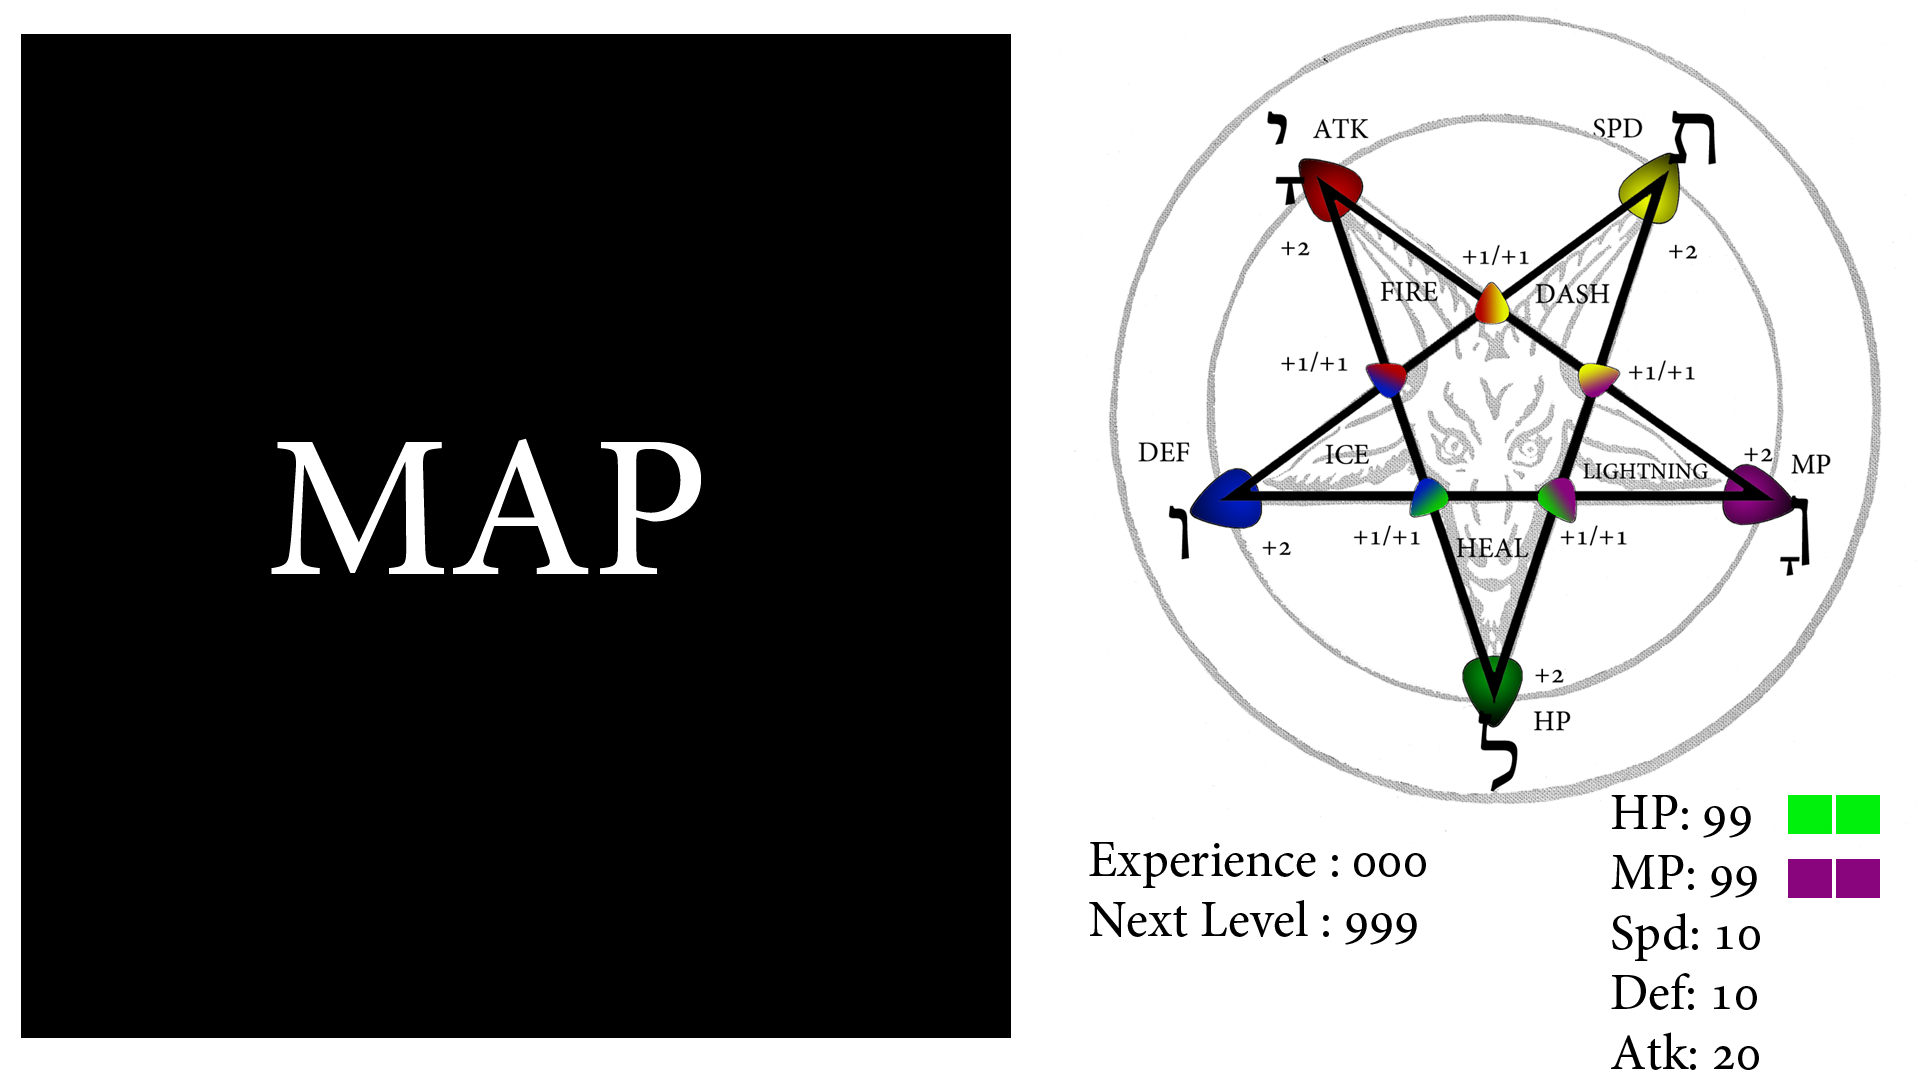
\includegraphics[width=5in]{Graphics/StatusMenu.png}
\caption{Level-Up and Map Screen.}
\label{LevelupScreen}
\end{figure}

\begin{figure}[h!]
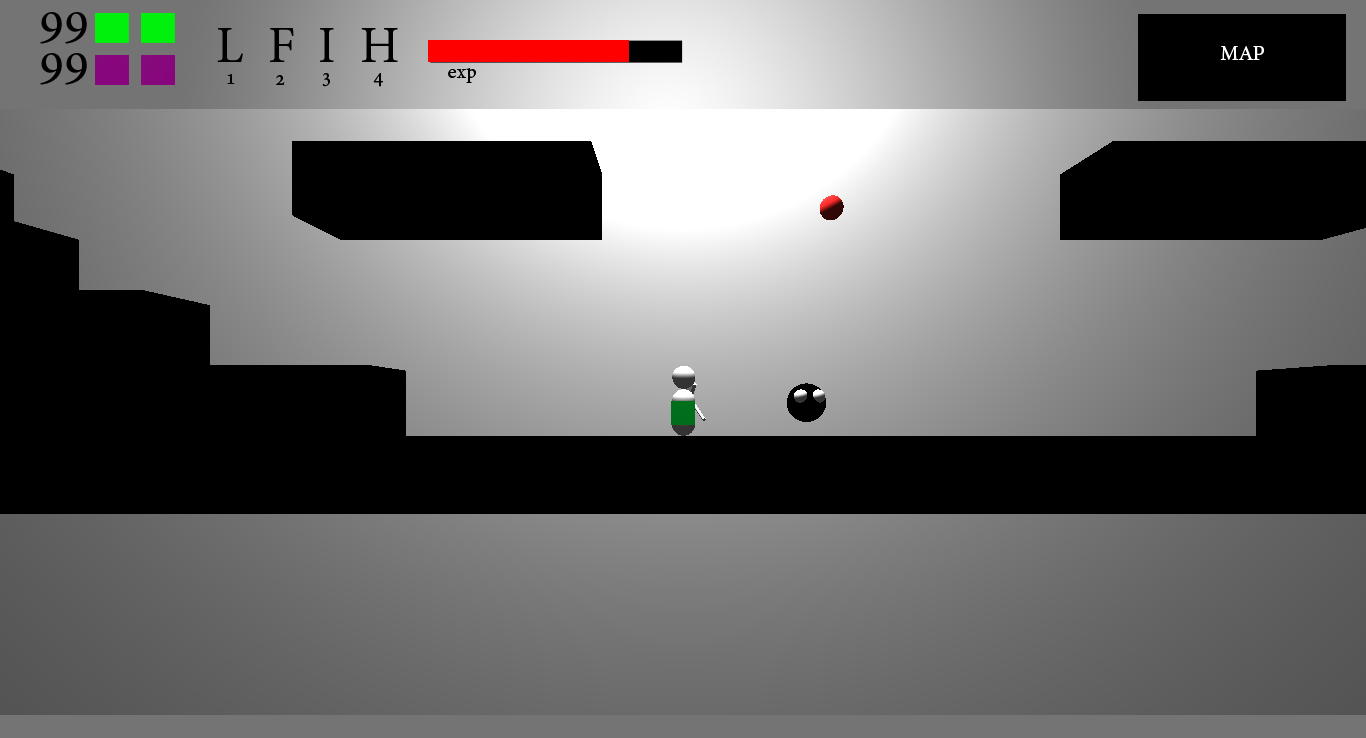
\includegraphics[width=5in]{Graphics/GameScene.png}
\caption{Game Scene.}
\label{GameScene}
\end{figure}


\section{Technical Risk}

Every software development project faces probable risks during its development process. Call of the Wintermoon is a promising video game with innovative features, and has its own technical risks.  In this section possible risks and appropriate strategies for dealing with each of them will be outlined.

\subsection{Meeting the deadline}
The deadline for completing the first demo is April 15th.  The main concern of the group is not meeting this deadline.  Call of the Wintermoon includes numerous features, characters and game objects.  For handling this problem development will be accomplished through multiple iterations.  In the first iterations the most important priority is to implement the basic functionalities, yielding a playable game.  In the next iteration the group will try to identify and prioritize remaining features.

\subsection{Scripting Animation}
Blender includes certain advanced features for 3D animation.  Some of these features (such as the inverse kinematics system) are not present in Unity.  As a result, some aspects of animations which are easily implemented in Blender may not be implementable in Unity.  This may cause the animation quality to suffer, or may require more effort than expected to achieve a reasonable solution.

\subsection{Dynamic level Generation}
The idea of dynamic level generation was one of the most interesting concepts in designing Call of the Wintermoon gameplay.  The fact that the player can play the whole game in a short sitting while also being able to acquire different abilities is quite interesting and there are not many games which offer this flexibility.  The current state of the random level generation is not very sophistocated, and doesn't adjust to any type of difficulty curve.  We plan to add these features, but are uncertain if it will be feasible to accomplish this in the limited time we have.


\label{StatsSection}
\section{Player and Enemy Statistics}

\begin{tabular}{|r|l|l|l|l|l|l|}
\hline
Entity & HP & MP & Attack & Defense & Speed & Experience Gained\\
\hline
Wyrm&30&0&10&0&10&1\\
F. Headman&60&0&30&0&20&5\\
Shadowman&100&0&60&10&20&10\\
Snowman&200&0&60&20&0&20\\
Shoggoth&400&0&100&50&5&40\\
Xl'Grhthbtrg&1500&0&100&30&30&100\\
Player (Initial)&299&299&20&10&10&N/A\\
\hline

\end{tabular}

\begin{tabular}{|r|l|}
\hline
Level-Up&Experience Required\\
\hline
1&50\\
2&100\\
3&200\\
4&400\\
5&800\\
\hline
\end{tabular}

\label{RoomAndEnemy}
\section{Room and Enemy Configurations}

Basic room configurations are listed in this section.  For a more complete listing, refer to the text files accompanied by the electronic submission.

\begin{tabular}{|r|l|}
\hline
\multicolumn{2}{|c|}{Legend} \\
\hline
Space & Empty space \\
* & Snow \\
@ & Rock \\
w & Wyrm \\
f & F. Headman \\
s & Shadowman \\
n & Snowman \\
h & Shoggoth \\
X & Xl'Grhthbtrg \\
\hline

\end{tabular}

\begin{figure}[htbp]
	%\makebox[\textwidth]{\hrulefill}{
	%\small
	\verbatiminput{Code/type1.txt}
	%\normalsize}
	\caption{Room type 1.}
	\label{Type1}
\end{figure}

\begin{figure}[htbp]
	%\makebox[\textwidth]{\hrulefill}{
	%\small
	\verbatiminput{Code/type2.txt}
	%\normalsize}
	\caption{Room type 2.}
	\label{Type2}
\end{figure}

\begin{figure}[htbp]
	%\makebox[\textwidth]{\hrulefill}{
	%\small
	\verbatiminput{Code/type3.txt}
	%\normalsize}
	\caption{Room type 3.}
	\label{Type3}
\end{figure}

\begin{figure}[htbp]
	%\makebox[\textwidth]{\hrulefill}{
	%\small
	\verbatiminput{Code/type4.txt}
	%\normalsize}
	\caption{Room type 4.}
	\label{Type4}
\end{figure}

\begin{figure}[htbp]
	%\makebox[\textwidth]{\hrulefill}{
	%\small
	\verbatiminput{Code/type5.txt}
	%\normalsize}
	\caption{Room type 5.}
	\label{Type5}
\end{figure}

\end{document}